\documentclass[journal]{IEEEtran}
\usepackage{iftex}
\ifPDFTeX
\else
\usepackage{fontspec}
\setmainfont{TeX Gyre Termes}
\setsansfont{TeX Gyre Heros}
\setmonofont{TeX Gyre Cursor}
\fi
\usepackage{amsmath,amssymb,booktabs,array,multirow,enumitem,algorithm,algpseudocode,microtype,graphicx,pgfplots,placeins}
\usepackage{cite}
\usepackage{tikz,adjustbox}
\usetikzlibrary{arrows.meta,positioning,calc,shapes.geometric}
\usepackage[caption=false,font=footnotesize]{subfig}
\usepackage{xurl}
\usepackage[hidelinks]{hyperref}
\hypersetup{pdftitle={BaitFL: Lightweight Trap-Based Free-Rider Detection and Mitigation in Federated Learning},pdfauthor={Aashnan Rahman},pdfkeywords={federated learning,free-rider detection,robust statistics}}
\pgfplotsset{compat=1.18}
\makeatletter
\setlength{\@fptop}{0pt}
\setlength{\@fpsep}{6pt plus 1pt minus 1pt}
\setlength{\@fpbot}{0pt plus 1fil}
\setlength{\@dblfptop}{0pt}
\setlength{\@dblfpsep}{6pt plus 1pt minus 1pt}
\setlength{\@dblfpbot}{0pt plus 1fil}
\makeatother
\setlength{\floatsep}{6pt plus 1pt minus 1pt}
\setlength{\dblfloatsep}{6pt plus 1pt minus 1pt}
\setlength{\textfloatsep}{6pt plus 1pt minus 1pt}
\setlength{\dbltextfloatsep}{6pt plus 1pt minus 1pt}
\setlength{\intextsep}{6pt plus 1pt minus 1pt}
\makeatletter
\renewcommand{\section}{\@startsection{section}{1}{\z@}{1.5ex}{0.7ex}{\normalfont\normalsize\centering\scshape}}
\renewcommand{\subsection}{\@startsection{subsection}{2}{\z@}{1.5ex}{0.7ex}{\normalfont\normalsize\itshape}}
\makeatother
\usepgfplotslibrary{groupplots,fillbetween}
\definecolor{honestblue}{HTML}{2878A5}
\definecolor{riderorange}{HTML}{D66B27}
\definecolor{baitteal}{HTML}{187F8C}
\definecolor{comparisongray}{HTML}{6C7078}
\providecommand*{\algorithmautorefname}{Algorithm}






\title{BaitFL: Lightweight Trap-Based Free-Rider Detection and Mitigation in Federated Learning}
\author{Aashnan~Rahman\thanks{Aashnan Rahman is with the Department of Computer Science and Engineering, Islamic University of Technology.}}
\begin{document}
\maketitle
\raggedbottom
\setlength{\parskip}{0pt plus 2pt minus 0.5pt}
\makeatletter
\def\@textbottom{\vskip\z@ plus 6pt}
\makeatother
\setlength{\abovedisplayskip}{6pt plus 1pt minus 1pt}
\setlength{\belowdisplayskip}{6pt plus 1pt minus 1pt}
\setlength{\abovedisplayshortskip}{3pt plus 1pt minus 1pt}
\setlength{\belowdisplayshortskip}{3pt plus 1pt minus 1pt}

\begin{abstract}
\bfseries
Free riders obtain the shared federated model without performing local
training, while fabricated responses can resemble genuine updates.
BaitFL audits this behavior through undisclosed model challenges,
update norms and layer-level profiles. Geometric tests and repeated fresh
evidence govern removal, while bounded review limits exclusion when
the evidence remains inconclusive. The server requires neither an
auxiliary detector nor client-reported loss or attack identities.
Experiments across three random seeds cover MNIST and CIFAR-10, IID and
non-IID partitions, four non-adaptive fabrication strategies, and 30\%
and 40\% free riders. All free riders in this main grid are removed, giving
100.00\% recall across 96 runs. There are 3
honest removals, concentrated in 2 runs. Additional
frozen-setting checks found no honest removal in four honest-only runs,
but FR2--FR4 were undetected at 5\% prevalence in the completed non-IID
tests. These results identify a lower-prevalence limitation. An oracle
norm-matching feature diagnostic also substantially reduces first-cycle
certification, exposing a limit to magnitude-based separation. In separately
timed 100-round runs, server-side checking accounted for 0.58\% of total
computation time on MNIST and 0.89\% on CIFAR-10.
BaitFL is lightweight in server computation
for the evaluated population of 100 clients. Even IID settings withhold
about 11\% of honest responses through auditing. Withheld contributions
and honest-client errors remain costs of the method, which requires
visibility of individual client responses.
\end{abstract}

\begin{IEEEkeywords}
federated learning, free-rider detection, hidden challenges, robust statistics,
non-IID data, client auditing
\end{IEEEkeywords}

\section{Introduction}

Federated learning (FL) allows multiple clients to train a shared model
without handing over their local data. In each communication round, the
server distributes the current global model, the clients update it using
their own data, and the server aggregates the returned updates into a
revised model~\cite{mcmahan2017communication}. Since raw data stays with
its owner, participants can collaborate without first creating a central
repository of their records. Keeping data local does not remove every
privacy risk, as shared updates can still reveal information about
training data~\cite{kairouz2021advances,zhu2019leakage,melis2019leakage}.
Exchanging updates instead of
datasets also avoids moving large volumes of local data, although repeated
model exchange remains a significant communication cost in
FL~\cite{mcmahan2017communication}. Effective collaboration depends on clients
performing useful local training, even though the server cannot directly
observe that work.

Like other distributed systems, FL is open to misconduct. Label-flipping and
model-poisoning attacks, for example, alter local data or submitted updates
in order to degrade the global model or introduce targeted
behavior~\cite{kairouz2021advances,bagdasaryan2020backdoor}. Free riding is
a quieter problem. The participant's primary aim is to obtain the shared
model without paying the cost of local
training~\cite{lin2019freeriders,fraboni2021freerider}. A client may lack
useful data or computational resources, or may simply choose to conserve
them. Instead of training, it can return an unchanged model, fabricate a
noisy response, or build an update from models received in earlier rounds.
Such responses may resemble what the server expects, so they need not
visibly disrupt learning and can evade checks aimed at overtly harmful
updates. Free riding shifts the training burden to honest participants. When
a client withholds useful data and computation, the federation also loses a
contribution that could have improved the shared model.
Figure~\ref{fig:free-rider-attack} shows the standard model exchange.
All clients receive the global model. Honest clients train it on local
data and return their local models, while a free rider submits a fabricated
model without local optimization.
\begin{figure}[t]
\centering

% BEGIN SOURCE: figures/free_rider_attack.tex (embedded vector drawing)
\adjustbox{max width=\columnwidth}{\begingroup
% BEGIN SOURCE: figures/diagram_style.tex

\pgfplotsset{compat=1.18}
\definecolor{challenge}{HTML}{187F8C}
\definecolor{removal}{HTML}{A33333}
\definecolor{honestblue}{HTML}{2878A5}
\definecolor{riderorange}{HTML}{D66B27}
\tikzset{
 every picture/.style={font=\normalfont\fontsize{11}{13}\selectfont},
 process/.style={rectangle,draw=black!65,line width=.5pt,
   align=center,minimum height=.85cm,inner sep=6pt},
 state/.style={process,rounded corners=5pt,minimum height=.9cm},
 flow/.style={-{Latex[length=2.2mm]},draw=black!65,line width=.6pt},
 feedback/.style={flow,dashed},
 note/.style={align=center,font=\normalfont\fontsize{10.5}{12}\selectfont},
 trap/.style={process,draw=challenge,text=challenge}
}

% END SOURCE: figures/diagram_style.tex

\definecolor{sharedmodel}{HTML}{7040B0}
\definecolor{honest}{HTML}{2878A5}
\definecolor{rider}{HTML}{D66B27}

\begin{tikzpicture}[font=\fontsize{10}{12}\selectfont,
 sent/.style={flow,draw=sharedmodel},
 trained/.style={flow,draw=honest},
 fabricated/.style={flow,draw=rider,dashed},
 card/.style={draw=black!45,rounded corners=3pt,line width=.6pt,
 minimum width=2.4cm,minimum height=2.7cm},
 key/.style={font=\fontsize{9}{11}\selectfont,anchor=west}]
\node[draw=black!60,rounded corners=3pt,minimum width=8.3cm,
 minimum height=1.8cm,line width=.65pt] (server) at (2.9,0) {};
\node[font=\bfseries\fontsize{11}{13}\selectfont] at (2.7,.48) {Federated server};
\node[font=\fontsize{9.5}{11}\selectfont] at (2.7,-.02) {Broadcast global model};
\node[font=\fontsize{9.5}{11}\selectfont] at (2.9,-.59)
 {Aggregate returned local models};
\foreach \y in {-.16,.12,.40} {
 \draw[black!60,rounded corners=.5pt] (-.85,\y-.09) rectangle (.35,\y+.09);
 \fill[honest] (-.68,\y) circle (.025);
 \draw[black!40] (-.5,\y)--(.17,\y);
}
\foreach \yy in {-.2,.32} { \foreach \zz in {-.3,.06,.42} {
 \draw[sharedmodel!45,line width=.4pt] (5.05,\yy)--(5.68,\zz);
 \draw[sharedmodel!45,line width=.4pt] (5.68,\zz)--(6.31,\yy);
}}
\foreach \xx/\yy in {5.05/-.2,5.05/.32,5.68/-.3,5.68/.06,5.68/.42,6.31/-.2,6.31/.32}
 \fill[sharedmodel] (\xx,\yy) circle (.035);
\foreach \xx/\id in {0/1,2.9/2} {
 \begin{scope}[shift={(\xx,-3.5)}]
  \node[card,draw=honest!75,fill=honest!3] {};
  \node[font=\bfseries,text=honest] at (0,.98) {Honest \id};
  \draw[honest,line width=.6pt] (-.93,-.05)--(-.93,.40)
   arc[start angle=180,end angle=360,x radius=.23,y radius=.08]
   --(-.47,-.05) arc[start angle=0,end angle=-180,x radius=.23,y radius=.08];
  \draw[honest,line width=.6pt] (-.70,.40) ellipse[x radius=.23,y radius=.08];
  \draw[black!65,rounded corners=1pt,line width=.6pt] (-.27,-.12) rectangle (.91,.56);
  \draw[black!65,line width=.6pt] (-.38,-.22)--(1.02,-.22)--(.88,-.34)--(-.24,-.34)--cycle;
  \begin{scope}[shift={(.32,.22)},x=.85cm,y=.7cm]
   \foreach \a in {-.3,.3} { \foreach \b in {-.4,0,.4} {
    \draw[honest!55,line width=.4pt] (-.45,\a)--(0,\b);
    \draw[honest!55,line width=.4pt] (0,\b)--(.45,\a);
   }}
   \foreach \nx/\ny in {-.45/-.3,-.45/.3,0/-.4,0/0,0/.4,.45/-.3,.45/.3}
    \fill[honest] (\nx,\ny) circle[radius=1pt];
  \end{scope}
  \node[font=\fontsize{9.5}{11}\selectfont] at (0,-.78) {Local training};
 \end{scope}
}
\begin{scope}[shift={(5.8,-3.5)}]
 \node[card,draw=rider!80,fill=rider!4] {};
 \node[font=\bfseries,text=rider] at (0,.98) {Free rider};
 \draw[black!65,rounded corners=1pt,line width=.6pt] (-.72,-.12) rectangle (.72,.56);
 \draw[black!65,line width=.6pt] (-.85,-.22)--(.85,-.22)--(.70,-.34)--(-.70,-.34)--cycle;
 \node[text=rider] at (0,.22) {$\widehat w_{t,i}$};
 \node[font=\fontsize{9.5}{11}\selectfont,align=center] at (0,-.78) {Skips local\\training};
\end{scope}
\foreach \xx in {0,2.9,5.8} {
 \draw[sent] (\xx-.16,-.90)--(\xx-.16,-2.15);
 \node[font=\fontsize{10}{12}\selectfont,text=sharedmodel,anchor=east]
  at (\xx-.31,-1.5) {$w_t$};
}
\foreach \xx in {0,2.9} \draw[trained] (\xx+.16,-2.15)--(\xx+.16,-.90);
\draw[fabricated] (5.96,-2.15)--(5.96,-.90);
\draw[sent] (-1.05,-5.35)--(-.40,-5.35);
\node[key,text=sharedmodel] at (-.25,-5.35) {Global model};
\draw[trained] (-.40,-5.91)--(-1.05,-5.91);
\node[key,text=honest] at (-.25,-5.91) {Trained local model};
\draw[fabricated] (-.40,-6.47)--(-1.05,-6.47);
\node[key,text=rider] at (-.25,-6.47) {Fabricated local model};
\draw[honest,line width=.55pt] (4.15,-6.08)--(4.15,-5.66)
 arc[start angle=180,end angle=360,x radius=.23,y radius=.08]
 --(4.61,-6.08) arc[start angle=0,end angle=-180,x radius=.23,y radius=.08];
\draw[honest,line width=.55pt] (4.38,-5.66) ellipse[x radius=.23,y radius=.08];
\node[key] at (4.82,-5.91) {Local data};
\end{tikzpicture}


\endgroup}
% END SOURCE: figures/free_rider_attack.tex

\caption{Free riding in federated learning. The server broadcasts the
global model. Honest clients return locally trained models, while a free
rider returns a fabricated model without local training.}
\label{fig:free-rider-attack}
\end{figure}

Detecting this omission is difficult because unusual updates are not limited
to free riders. Honest clients differ in sample sizes, class distributions,
and local learning trajectories, particularly under non-IID
data~\cite{kairouz2021advances}. A small update can therefore reflect
legitimate training, while a fabricated one can look like an ordinary
contribution. The server has to tell these cases apart without observing
local optimization. Existing approaches rely on learned anomaly models,
parameter audits, or evidence obtained through inference
attacks~\cite{lin2019freeriders,wang2024pass,recasens2026frida}. This raises a
practical question: can lightweight server-side checks detect free riding
without training an auxiliary detector? There is also a cost to being wrong.
Withholding an honest client's updates can reduce its contribution to the shared
model, even if it is never permanently removed. A detector must therefore
consider both the evidence needed for removal and the duration of temporary
exclusion.

To address this problem, we propose \emph{BaitFL}, a lightweight trap-based
method for detecting and mitigating free riders in federated learning.
In the 96-run main grid at 30\% and 40\% prevalence,
it removes all tested free riders,
with 3 honest removals in 2 runs. Checking
accounts for less than 1\% of computation in the instrumented executions.
Additional low-prevalence and norm-matching checks expose limits to this
result rather than supporting prevalence-independent detection.

\noindent The main contributions of this work are as follows:
\begin{itemize} %
\item \textbf{Lightweight server-side detection.} We develop a challenge-based
detector using update norms and tensor profiles, without training an auxiliary
detection model or accessing clients' private training data.
\item \textbf{Confirmation using repeated evidence.} We design a decision
mechanism that separates initial suspicion from permanent removal and requires
fresh evidence of the same component across two challenges and distinct audit
cycles for statistical confirmation.
\item \textbf{Bounded mitigation and rehabilitation.} We retain strong evidence
across ambiguous cycles while allowing unconfirmed quarantine to expire and
clearing statistical memory after repeated clean observations.
\item \textbf{Evaluation across four free-rider behaviors.} We study unchanged-model
responses, random fabrication, history averaging, and trajectory imitation on
MNIST and CIFAR-10 under IID and non-IID partitions, with 30\% and 40\% free riders.
\end{itemize}

Sections~\ref{sec:related} and~\ref{sec:threat} review related work and
define the threat model. Section~\ref{sec:method} presents the auditing
procedure, followed by results in Section~\ref{sec:results} and complexity
analysis in Section~\ref{sec:complexity}. Section~\ref{sec:discussion}
discusses security, limitations and future work before the conclusion.

\section{Literature Review}\label{sec:related}
Free-rider detection concerns omitted training, whereas poisoning
defenses primarily address harmful updates. Lin \emph{et al.} introduced
fabrication attacks and STD-DAGMM, combining update statistics with an
autoencoder and mixture model~\cite{lin2019freeriders,zong2018dagmm}.
Fraboni \emph{et al.} studied unchanged-model and disguised, decaying-noise
responses in model aggregation~\cite{fraboni2021freerider}. Zhu \emph{et al.}
developed scaled-delta and advanced attacks that imitate training
trajectories~\cite{zhu2021advanced}. These studies show why an attacker
need not submit an obviously damaging response. They also motivate
testing magnitude-matched fabrication rather than assuming every free
rider produces a small update.

Learned detectors and contribution audits obtain different kinds of
evidence. STD-DAGMM requires auxiliary fitting, whose cost depends on
architecture and training budget. FRAD combines learned detection with
contribution estimates and reputation~\cite{wang2024frad}. Its additional
context depends on reliable resource and contribution information.
PASS asks clients to evaluate peers' models on local data and report
contribution scores~\cite{wang2024pass}. It avoids central access to raw
data, but adds peer evaluation and exposes models to auditors. Low
utility on an evaluator's data can also reflect heterogeneity rather
than omitted training.

FRIDA uses membership and property inference as training
evidence~\cite{recasens2026frida}. Its membership variants introduce
canaries and client training work, while property variants infer local
dataset characteristics. These are distinct information and computation
tradeoffs, not direct inspection of raw records. BaitFL likewise has a
privacy limit: attributable responses must remain visible. It cannot
operate unchanged behind secure aggregation~\cite{bonawitz2017practical},
and keeping raw data local does not prevent leakage through
updates~\cite{zhu2019leakage,melis2019leakage}.

Robust aggregation offers another point of comparison. Krum, trimmed
aggregation and geometric-median methods reduce the effect of Byzantine
updates~\cite{blanchard2017krum,yin2018byzantine,pillutla2022rfa}.
FLTrust uses a trusted server dataset~\cite{cao2021fltrust}. These methods
aim to protect learning under their assumptions; rejecting a harmful
update does not establish whether its sender trained. FedProx, SCAFFOLD
and FedNova address heterogeneous local optimization
\cite{li2020fedprox,karimireddy2020scaffold,wang2020fednova}. They can
improve honest training but do not, by themselves, audit a participant
that skips the prescribed computation.

Proof-of-learning and VeriML seek evidence about executed training or
outsourced learning computations~\cite{jia2021prooflearning,zhao2021veriml}.
They provide a different assurance from population-relative anomaly
scores and require their own verification artifacts. Data-Shapley and
federated valuation estimate marginal usefulness
\cite{ghorbani2019datashapley,jia2019datavaluation,liu2022gtgshapley};
usefulness remains different from evidence of honest participation.

BaitFL tests responses to altered starting models using compact
statistics and repeated evidence. Our comparisons cover different
endpoints: no-defense aggregation for utility, a declared STD-DAGMM
implementation for timing and flag diagnostics, and published information
requirements qualitatively. They do not constitute a common-workload
ranking against PASS, FRAD or FRIDA. Supplementary Table~S1 retains the
detailed requirements comparison.

\section{Threat Model}\label{sec:threat}
\subsection{Participants and Server Knowledge}
A trusted server coordinates $N$ clients with persistent identities and
reliable communication. Every active client responds in each round.
The population is fixed, with no client sampling, late arrivals or dropouts.
Removal ends participation. Quarantined clients still return responses,
but those responses are excluded from aggregation, as are all responses to
traps. Honest clients train the model they receive with the prescribed
optimizer. Their datasets may differ in size and class distribution,
covering both IID and non-IID partitions.

The server may send different models to different clients without disclosing
which are traps. For client $i$ in round $t$, it knows the sent model,
$w^{\rm send}_{t,i}$, and the returned model, $w^{\rm ret}_{t,i}$. These give
the update and its norm,
\begin{equation}
 \Delta_{t,i}=w^{\rm ret}_{t,i}-w^{\rm send}_{t,i},\qquad
 r_{t,i}=\|\Delta_{t,i}\|_2.
\end{equation}
Detection uses these responses and the server's audit history. The server
has no access to private training records and no prior knowledge of which
clients are free riders or how they construct their responses.
Individual responses are visible to it, so the setting does not use
secure aggregation.

\subsection{Free-Rider Objective and Scope}
Free riders seek the shared model while avoiding local training costs.
Some lack suitable data or training resources. Others have both but choose
to withhold them. They can still receive and store models and carry out
the relatively simple calculations needed to fabricate a response.
Introducing a targeted error or backdoor is outside their objective here.

Our experiments consider persistent free riding without collusion,
following Lin \emph{et al.}~\cite{lin2019freeriders}. These clients perform
no local optimization at any stage. Partial training and behavior that
alternates between training and free riding fall outside this scope.
Each attacker relies only on its own received-model history and local
randomness. They do not share responses or change identities.
The evaluated strategies do not attempt to recognize traps or adapt to
evade audits. Section~\ref{sec:evasion} discusses those possibilities.

We assume an honest majority because screening uses peer statistics and
seeks a separated minority of suspicious responses. The experiments use
30\% and 40\% free riders, with one fixed fabrication strategy shared by
the free riders in each run.

\subsection{Evaluated Free-Rider Behaviors}
Let $\widehat w_{t,i}$ denote the model returned by a free rider.
All four strategies below skip local optimization.

\par\medskip\noindent\textbf{FR1: current-model sendback.}\par\nopagebreak\smallskip\noindent
Returning the received model unchanged gives a zero update, whether the
model is ordinary or a trap:
\begin{equation}
 \widehat w_{t,i}=w^{\rm send}_{t,i}.
\end{equation}

\par\medskip\noindent\textbf{FR2: bounded random fabrication.}\par\nopagebreak\smallskip\noindent
Independent uniform noise is added to each floating point entry of the
received model state:
\begin{equation}
 \widehat w_{t,i}=w^{\rm send}_{t,i}+\epsilon_{t,i},\quad
 (\epsilon_{t,i})_j\sim\mathcal U(-10^{-3},10^{-3}).
\end{equation}

\par\medskip\noindent\textbf{FR3: received-history averaging.}\par\nopagebreak\smallskip\noindent
With a history length $H$, the response averages the most recent
$\min(H,t)$ received model states, stored in $\mathcal H_{t,i}$:
\begin{equation}
 \widehat w_{t,i}=\frac{1}{|\mathcal H_{t,i}|}
       \sum_{w\in\mathcal H_{t,i}}w.
\end{equation}
This history includes the current model and any earlier traps. The client
therefore follows recent model evolution without training on local data.

\par\medskip\noindent\textbf{FR4: received-trajectory imitation.}\par\nopagebreak\smallskip\noindent
Changes between consecutive received models provide an estimated update.
Let $\overline d_{t,i}$ average up to the five most recent differences:
\begin{align}
 d_{s,i}&=w^{\rm send}_{s,i}-w^{\rm send}_{s-1,i},\\
 \widehat w_{t,i}&=w^{\rm send}_{t,i}+\overline d_{t,i}+\eta_{t,i}.
\end{align}
For a standard Gaussian vector $z_{t,i}$, the noise is scaled as
\begin{equation}\label{eq:fr4-noise}
 \eta_{t,i}=0.1\,
 \frac{\max(\|\overline d_{t,i}\|_2,\epsilon_0)}
      {\max(\|z_{t,i}\|_2,\epsilon_0)}\,z_{t,i},
 \qquad\epsilon_0=10^{-6}.
\end{equation}
Equation~\eqref{eq:fr4-noise} applies to vectors covering all floating
model entries. On the first response,
$\overline d_{1,i}=0$ and $\eta_{1,i}$ instead has independent Gaussian entries with
standard deviation $10^{-4}$. Traps enter the same history as ordinary
models and affect the estimated trajectory.


\section{Proposed Methodology}\label{sec:method}
BaitFL compares clients through hidden model challenges, then separates
initial suspicion from the evidence needed for removal.
Figure~\ref{fig:audit-schedule} shows the round schedule,
Figure~\ref{fig:challenge-mechanism} shows the challenge mechanism, and
Figure~\ref{fig:client-states} summarizes client participation states.
Warmup establishes an ordinary training trajectory
(Phase I). Paired coverage collects comparable responses
(Phase II), and confirmation updates the client records
(Phase III). Outside paired cycles, ordinary training
continues with sparse audits (Phase IV).

The server first runs warmup and initial paired coverage. Thereafter, it
repeats paired cycles while any client has an active review budget or
rehabilitation probation. Otherwise, it executes ordinary rounds and any
scheduled sparse audit until the training horizon $T$ is reached. The
continuation rules appear at the bottom of Figure~\ref{fig:audit-schedule}.
The illustrated second paired cycle permits earliest removal at round 30.
The example then enters ordinary training with audits after ten quiet rounds.
The two challenge labels summarize exposures within each paired cycle.
The records $\mathcal S$ retain client status, quarantine, review budget,
component counts, clean progress and cooldown. Counts start at zero and
the quiet clock is initially unset, $\sigma=\bot$. The study uses warmup length
$T_{\rm warm}=10$, paired-cycle length $\ell_{\rm cyc}=10$ and sparse-audit interval $I=10$.

The challenge changes a client's starting point without changing the
requested training task. Honest optimization responds to that starting
point through the local data. An unchanged response, arbitrary noise or
recycled model history need not respond in the same way. Comparing
clients that received the same challenge can expose differences in the
size and layer distribution of their updates. Two independent challenges
test whether the difference recurs. This is behavioral evidence rather
than proof of training, since fabricated and genuine responses may still
overlap.

% BEGIN SOURCE: generated/notation_settings.tex
\begin{table*}[t]\centering\footnotesize
\renewcommand{\arraystretch}{1.05}
\caption{Principal notation and fixed protocol settings.}\label{tab:notation-settings}
\begin{tabular}{>{\raggedright\arraybackslash}p{3.1cm}>{\raggedright\arraybackslash}p{8.0cm}>{\raggedright\arraybackslash}p{4.8cm}}\toprule
Symbol & Meaning & Study setting \\ \midrule
$N,T$ & Initial client population and training horizon & 100 clients, 100 rounds \\
$w_t,\tau_A,\tau_B$ & Global model and the two shared challenges & Updated globally, fixed per cycle \\
$\Delta_i^a,r_i^a,p_i^a$ & Response change, its norm and its tensor profile & Measured from returned models \\
$z_i^{n,a},z_i^{p,a}$ & Leave-one-out norm and profile scores & Population-derived \\
$T_{\rm warm},\ell_{\rm cyc},I$ & Warmup, paired-cycle length and sparse-audit interval & 10, 10 and 10 rounds \\
$\gamma,\epsilon_\tau$ & Relative challenge strength and tensor-scale floor & $0.01$, $10^{-4}$ \\
$B$ & Bootstrap replicates & 1,000 \\
$P,L$ & Floating model coordinates and floating tensors & Architecture-dependent \\
$\mathcal U,\mathcal V$ & Nominated cohort and remaining active peers & Statistical certification sets \\
$\mathcal S,\mathcal E$ & Client records and paired cycle decisions & Retained state and fresh evidence \\
$\mathsf{strong}$, $\mathsf{unresolved}$, $\mathsf{clear}$ & Cycle outcomes & Distinct from retained client status \\
$\mathcal F,\mathcal D,\mathcal F_{\rm elig}$ & Sparse findings, cooldown clients and eligible findings & $\mathcal F_{\rm elig}=\mathcal F\setminus\mathcal D$ \\
$\mathcal W_{\rm det}$ & Total detector work over the training horizon & Bound in Section~\ref{sec:complexity} \\
\bottomrule\end{tabular}
\end{table*}

% END SOURCE: generated/notation_settings.tex


\begin{figure}[t]
\centering

% BEGIN SOURCE: figures/audit_schedule.tex (embedded vector drawing)
\adjustbox{max width=\columnwidth}{\begingroup
% BEGIN SOURCE: figures/diagram_style.tex

\pgfplotsset{compat=1.18}
\definecolor{challenge}{HTML}{187F8C}
\definecolor{removal}{HTML}{A33333}
\definecolor{honestblue}{HTML}{2878A5}
\definecolor{riderorange}{HTML}{D66B27}
\tikzset{
 every picture/.style={font=\normalfont\fontsize{11}{13}\selectfont},
 process/.style={rectangle,draw=black!65,line width=.5pt,
   align=center,minimum height=.85cm,inner sep=6pt},
 state/.style={process,rounded corners=5pt,minimum height=.9cm},
 flow/.style={-{Latex[length=2.2mm]},draw=black!65,line width=.6pt},
 feedback/.style={flow,dashed},
 note/.style={align=center,font=\normalfont\fontsize{10.5}{12}\selectfont},
 trap/.style={process,draw=challenge,text=challenge}
}

% END SOURCE: figures/diagram_style.tex


\begin{tikzpicture}[font=\fontsize{9.5}{11}\selectfont,
 note/.style={font=\fontsize{9}{10.5}\selectfont,align=center}]
\draw[black!55,line width=.55pt] (0,.65) rectangle (1.5,2.05);
\node[align=center] at (.75,1.55) {Warmup};
\node[note] at (.75,.96) {10 rounds};
\draw[challenge,line width=.7pt] (1.5,.65) rectangle (3,2.05);
\node[align=center,text=challenge] at (2.25,1.55) {Paired\\cycle 1};
\node[note,text=challenge] at (2.25,.92) {$\tau_A,\tau_B$};
\draw[challenge,line width=.7pt] (3,.65) rectangle (4.5,2.05);
\node[align=center,text=challenge] at (3.75,1.55) {Paired\\cycle 2};
\node[note,text=challenge] at (3.75,.92) {$\tau_A,\tau_B$};
\draw[black!55,line width=.55pt] (4.5,.65) rectangle (7.8,2.05);
\node[align=center] at (6.15,1.4) {Ordinary\\training};
\draw[flow] (0,.25)--(8.05,.25);
\node[note,anchor=east] at (-.12,.25) {$t$};
\foreach \xx/\rr in {0/0,1.5/10,3/20,4.5/30,6/40,7.5/50} {
 \draw[black!55,line width=.55pt] (\xx,.18)--(\xx,.32);
 \node[below=3pt] at (\xx,.18) {\rr};
}
\foreach \xx in {6,7.5} {
 \node[diamond,draw=challenge,line width=.65pt,minimum size=5pt,inner sep=0pt]
  at (\xx,.25) {};
}
\draw[removal,line width=.55pt] (4.5,-.34)--(4.5,-.56);
\node[note,text=removal] at (4.5,-.94) {Earliest\\removal};
\node[diamond,draw=challenge,line width=.65pt,minimum size=5pt,inner sep=0pt]
 at (6.35,-.94) {};
\node[note,anchor=west,text=challenge] at (6.58,-.94) {Audit};
\node[note,anchor=west] at (0,-1.72) {Review / probation};
\draw[feedback] (3.35,-1.72)--(4.05,-1.72);
\node[note,anchor=west,text=challenge] at (4.25,-1.72) {Repeat paired cycles};
\node[note,anchor=west] at (0,-2.25) {Neither active};
\draw[flow] (3.35,-2.25)--(4.05,-2.25);
\node[note,anchor=west] at (4.25,-2.25) {Ordinary + audit};
\end{tikzpicture}


\endgroup}
% END SOURCE: figures/audit_schedule.tex

\caption{Illustrative round schedule from warmup and paired coverage
to ordinary training with sparse audits.}
\label{fig:audit-schedule}
\end{figure}

\subsection{Challenges, Measurements, and Aggregation}
Each paired cycle starts from a frozen copy $w^{(c)}$ of the current global
model. For floating tensor $k$, the server creates traps $A$ and $B$ as
\begin{equation}\label{eq:trap}
 \tau_{a,k}=w^{(c)}_k+
 \gamma\max\{\operatorname{sd}(w^{(c)}_k),\epsilon_\tau\}\xi_{a,k},
 \quad a\in\{A,B\}.
\end{equation}
In~\eqref{eq:trap}, $\xi_{a,k}\sim\mathcal N(0,I)$ uses independent draws, and
$\operatorname{sd}$ is the tensor's population standard deviation. The
study sets $\gamma=0.01$ and $\epsilon_\tau=10^{-4}$. Floating buffers,
including BatchNorm statistics, are perturbed along with weights.
Integer counters remain unchanged. The two traps stay fixed within the
cycle, even as ordinary responses update the global model.

For a response to trap $a$, write $\Delta^a_{i,k}$ for the returned tensor
minus the tensor sent to client $i$. Its norm $r_i^a$ measures total update
magnitude. The scale-free profile in~\eqref{eq:profile} is
\begin{equation}\label{eq:profile}
 p^a_{i,k}=\frac{\|\Delta^a_{i,k}\|_2}
                  {\sum_j\|\Delta^a_{i,j}\|_2}.
\end{equation}
The profile is zero when its denominator is below $10^{-6}$. Otherwise,
it records where the update magnitude lies across floating tensors.

For each trap, client $i$ is compared with all other active clients having
a selected response to that same trap. Quarantined and unresolved clients
are not removed from this reference. Let $m_i^a$ and $d_i^a$ be the median
and median absolute deviation (MAD) of the peer norms. Then
\begin{equation}\label{eq:norm-score}
 z_i^{n,a}=\frac{r_i^a-m_i^a}{d_i^a/\Phi^{-1}(0.75)},
\end{equation}
where $\Phi$ is the standard normal cumulative distribution function.
The factor normalizes the MAD. It does not assume that client updates
are normally distributed.

The profile reference $\widetilde p_{-i}^a$ is the coordinatewise median
of the peer profiles. The implementation uses the lower middle value
when a tensor coordinate has an even number of peer observations.
Define the client's profile distance as
$\rho_i^a=\|p_i^a-\widetilde p_{-i}^a\|_2$. Peer distances are computed
against that same reference. Their median $\mu_i^a$ and MAD $\delta_i^a$
give
\begin{equation}\label{eq:profile-score}
 z_i^{p,a}=\frac{\rho_i^a-\mu_i^a}
                  {\delta_i^a/\Phi^{-1}(0.75)}.
\end{equation}
A missing comparison or zero MAD leaves the corresponding score undefined.

Send-back is checked separately. It means an exactly zero floating-point
update norm, or a returned model whose fingerprint matches the immediately
previous model sent to that client. The latter comparison covers every
tensor in the model state. The server retains one previous-sent fingerprint
per client, not a history of full returned models.

\begin{figure*}[t]
\centering
\subfloat[Challenge construction and comparison. Each group receives both
perturbed models, and the server compares norms and tensor profiles among
clients receiving the same trap.\label{fig:challenge-path}]{%
\parbox[c][5.5cm][c]{.53\textwidth}{\centering

% BEGIN SOURCE: figures/challenge_path.tex (embedded vector drawing)
\adjustbox{max width=\linewidth,max totalheight=5.4cm}{\begingroup
% BEGIN SOURCE: figures/diagram_style.tex

\pgfplotsset{compat=1.18}
\definecolor{challenge}{HTML}{187F8C}
\definecolor{removal}{HTML}{A33333}
\definecolor{honestblue}{HTML}{2878A5}
\definecolor{riderorange}{HTML}{D66B27}
\tikzset{
 every picture/.style={font=\normalfont\fontsize{11}{13}\selectfont},
 process/.style={rectangle,draw=black!65,line width=.5pt,
   align=center,minimum height=.85cm,inner sep=6pt},
 state/.style={process,rounded corners=5pt,minimum height=.9cm},
 flow/.style={-{Latex[length=2.2mm]},draw=black!65,line width=.6pt},
 feedback/.style={flow,dashed},
 note/.style={align=center,font=\normalfont\fontsize{10.5}{12}\selectfont},
 trap/.style={process,draw=challenge,text=challenge}
}

% END SOURCE: figures/diagram_style.tex


\begin{tikzpicture}
\node[process,text width=1.6cm] (frozen) at (0,0) {Frozen model\\$w^{(c)}$};
\node[trap,text width=1cm] (a) at (2.4,.9) {$\tau_A$};
\node[trap,text width=1cm] (b) at (2.4,-.9) {$\tau_B$};
\node[process,text width=1.6cm] (ca) at (4.7,.9) {Group $g$};
\node[process,text width=1.6cm] (cb) at (4.7,-.9) {Group $g$};
\node[process,text width=2cm,minimum height=2.4cm] (summary) at (7.4,0)
 {Compare peers\\[7pt]$r_i^a,\ p_i^a$\\[7pt]$z_i^{n,a},\ z_i^{p,a}$};
\draw[flow,draw=challenge] (frozen.east)--(a.west);
\draw[flow,draw=challenge] (frozen.east)--(b.west);
\draw[flow,draw=challenge] (a.east)--(ca.west);
\draw[flow,draw=challenge] (b.east)--(cb.west);
\draw[flow] (ca.east)--(summary.north west);
\draw[flow] (cb.east)--(summary.south west);
\node[note,text=challenge] at (2.4,1.65) {Independent perturbations};
\node at (3.5,-2.05) {$D_i^a=z_i^{p,a}-z_i^{n,a}$};
\end{tikzpicture}


\endgroup}
% END SOURCE: figures/challenge_path.tex
}}
\hfill
\subfloat[Recorded response geometry. CIFAR-10, non-IID data, FR3, 40\%
free riders, round 20. Axes show transformed paired mean scores.
\label{fig:challenge-scores}]{%
\parbox[c][5.5cm][c]{.43\textwidth}{\centering

% BEGIN SOURCE: figures/challenge_scores.tex (embedded vector drawing)
\adjustbox{max width=\linewidth,max totalheight=5.4cm}{\begingroup
% BEGIN SOURCE: figures/diagram_style.tex

\pgfplotsset{compat=1.18}
\definecolor{challenge}{HTML}{187F8C}
\definecolor{removal}{HTML}{A33333}
\definecolor{honestblue}{HTML}{2878A5}
\definecolor{riderorange}{HTML}{D66B27}
\tikzset{
 every picture/.style={font=\normalfont\fontsize{11}{13}\selectfont},
 process/.style={rectangle,draw=black!65,line width=.5pt,
   align=center,minimum height=.85cm,inner sep=6pt},
 state/.style={process,rounded corners=5pt,minimum height=.9cm},
 flow/.style={-{Latex[length=2.2mm]},draw=black!65,line width=.6pt},
 feedback/.style={flow,dashed},
 note/.style={align=center,font=\normalfont\fontsize{10.5}{12}\selectfont},
 trap/.style={process,draw=challenge,text=challenge}
}

% END SOURCE: figures/diagram_style.tex


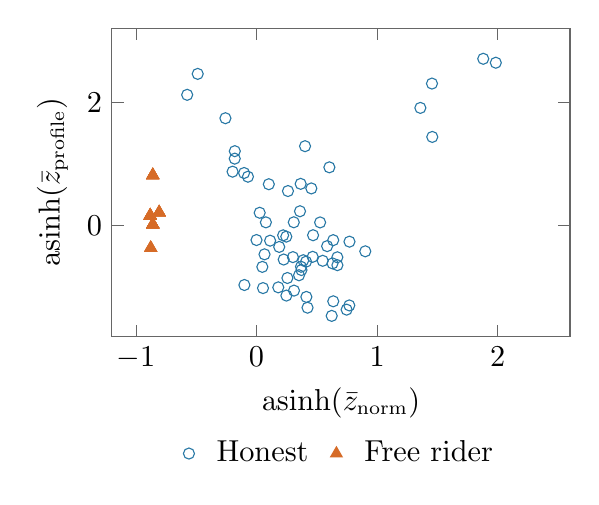
\begin{tikzpicture}
\begin{axis}[width=7.4cm,height=5.5cm,
 xmin=-1.2,xmax=2.6,ymin=-1.8,ymax=3.2,
 xlabel={$\operatorname{asinh}(\bar z_{\rm norm})$},
 ylabel={$\operatorname{asinh}(\bar z_{\rm profile})$},
 label style={font=\fontsize{10.5}{12}\selectfont},
 tick label style={font=\fontsize{10.5}{12}\selectfont},
 axis line style={black!60},tick style={black!60},
 legend style={draw=none,font=\fontsize{10.5}{12}\selectfont,
 at={(.5,-.30)},anchor=north,legend columns=2,/tikz/column sep=6pt},
 legend cell align=left,scaled ticks=false]
\addplot[only marks,mark=o,mark size=2pt,draw=honestblue]
 table[x=x,y=y,row sep=\\] {% PLOT DATA: generated/visuals/scatter_cifar10_40_noniid_FR3_0.dat (60 data rows)
x y \\
0.6701794546474221 -0.5121170611476913 \\
0.11262754653086965 -0.2427677065743296 \\
0.7707552339816854 -0.2587920822940484 \\
0.46890982985159446 -0.15451925988323942 \\
-0.1007567756067337 -0.9611150693508578 \\
0.6233887460937093 -1.4616112014815092 \\
0.30887071823926066 0.05526296744521777 \\
0.5487481457692832 -0.5689932838593805 \\
0.22058916174574547 -0.15626731042171543 \\
0.04815874270948856 -0.6674994522564285 \\
0.06606808200669567 -0.4641939015555078 \\
0.7471596536191437 -1.3605723347560228 \\
-0.4879351674147808 2.460089839957911 \\
0.18813407657757952 -0.34406595574219884 \\
0.3523663906070874 -0.8031843782784643 \\
1.8803413079565512 2.704795813923107 \\
0.6302031827223412 -0.610899789194286 \\
0.7694428848325895 -1.2921112869368052 \\
0.410836635362308 -0.5832564912505601 \\
0.6041300218324299 0.9456514413698807 \\
0.4655664855092439 -0.5047427348035345 \\
-0.19880158821032126 0.8754015496884053 \\
0.18040452449769026 -0.9992818298201369 \\
0.36591251597117713 0.6781144148314275 \\
0.5273429603649553 0.053001391875643546 \\
0.9019825057992666 -0.41528503117336574 \\
0.07744608989344086 0.05407290938397404 \\
0.24751236046027145 -1.1326098111263574 \\
-0.07133551987030641 0.7938196405516135 \\
-0.18092297986365466 1.0864477571668718 \\
0.2560410996129003 -0.8477892474107666 \\
0.454582131880149 0.6038499290526959 \\
1.9845855947985613 2.6408026015234576 \\
-0.5753027068374195 2.1207167095308272 \\
0.4229523689271172 -1.328844388952915 \\
0.3106179458024558 -1.0521626823156212 \\
0.6360116100937022 -0.23454591282969084 \\
0.4023262264350657 1.288369714715956 \\
0.02604377234055962 0.20936547495061858 \\
0.3016569714973536 -0.5093414228721875 \\
0.636279261784757 -1.2254451428135091 \\
0.4133452336599654 -1.1542056672073984 \\
-0.25813710814903573 1.7416860560926883 \\
0.05364838670912452 -1.0111199543188256 \\
0.3603662236252994 0.23399331541980714 \\
-0.18035978932833316 1.2076446055325043 \\
0.1017822653174671 0.6719089906722611 \\
0.5854220108033455 -0.33123831825264055 \\
0.3879963688945996 -0.5597784294244804 \\
-0.0002718635078779445 -0.23261789329503774 \\
-0.10331157578523108 0.8538812643207765 \\
0.36880721349623075 -0.6652404950369758 \\
0.37240388069059194 -0.7186724541113371 \\
0.2606511276930795 0.5615147309768543 \\
0.2468264282340247 -0.17715950310494497 \\
1.4552050399427474 2.3030504311290128 \\
0.22522787394140123 -0.5483771651311298 \\
1.4576588679665357 1.4385011178922262 \\
0.6706701429267402 -0.6396089872230084 \\
1.3588323536455238 1.909026473350222 \\
};
\addlegendentry{Honest}
\addplot[only marks,mark=triangle*,mark size=2.4pt,draw=riderorange,fill=riderorange]
 table[x=x,y=y,row sep=\\] {% PLOT DATA: generated/visuals/scatter_cifar10_40_noniid_FR3_1.dat (40 data rows)
x y \\
-0.860343767913979 0.018614384514417125 \\
-0.807957146590587 0.21515852973343477 \\
-0.8607200157670079 0.8160665193510424 \\
-0.8776775545420457 -0.3620265770334066 \\
-0.8607200157670079 0.8160665193510424 \\
-0.8776775545420457 -0.3620265770334066 \\
-0.8819898192740541 0.16282071406316093 \\
-0.8819898192740541 0.16282071406316093 \\
-0.8607200157670079 0.8160665193510424 \\
-0.860343767913979 0.018614384514417125 \\
-0.8819898192740541 0.16282071406316093 \\
-0.8819898192740541 0.16282071406316093 \\
-0.860343767913979 0.018614384514417125 \\
-0.8819898192740541 0.16282071406316093 \\
-0.860343767913979 0.018614384514417125 \\
-0.8819898192740541 0.16282071406316093 \\
-0.8607200157670079 0.8160665193510424 \\
-0.807957146590587 0.21515852973343477 \\
-0.860343767913979 0.018614384514417125 \\
-0.8607200157670079 0.8160665193510424 \\
-0.807957146590587 0.21515852973343477 \\
-0.8607200157670079 0.8160665193510424 \\
-0.8776775545420457 -0.3620265770334066 \\
-0.807957146590587 0.21515852973343477 \\
-0.8819898192740541 0.16282071406316093 \\
-0.8819898192740541 0.16282071406316093 \\
-0.8607200157670079 0.8160665193510424 \\
-0.807957146590587 0.21515852973343477 \\
-0.8819898192740541 0.16282071406316093 \\
-0.8607200157670079 0.8160665193510424 \\
-0.8607200157670079 0.8160665193510424 \\
-0.860343767913979 0.018614384514417125 \\
-0.8607200157670079 0.8160665193510424 \\
-0.8819898192740541 0.16282071406316093 \\
-0.860343767913979 0.018614384514417125 \\
-0.860343767913979 0.018614384514417125 \\
-0.807957146590587 0.21515852973343477 \\
-0.8776775545420457 -0.3620265770334066 \\
-0.8819898192740541 0.16282071406316093 \\
-0.860343767913979 0.018614384514417125 \\
};
\addlegendentry{Free rider}
\end{axis}
\end{tikzpicture}


\endgroup}
% END SOURCE: figures/challenge_scores.tex
}}
\caption{Model challenges and representative client responses.
Point shapes identify evaluation labels unavailable to the detector.
Panel (b) contains 40 free riders, but coincident score pairs leave only
about four distinct triangle locations visible.}
\label{fig:challenge-mechanism}
\end{figure*}

The representative response geometry in Figure~\ref{fig:challenge-scores}
uses the seed-42 execution. The plotted averages summarize the two
challenges and do not replace the paired component certificates.

Aggregation runs alongside these checks. Let $\mathcal A_t$ contain clients
that received the ordinary model and were not quarantined at the start of
round $t$, excluding any newly quarantined or removed at its end. Then
\begin{equation}\label{eq:method-aggregation}
 w_{t+1}=w_t+\frac{1}{|\mathcal A_t|}
                 \sum_{i\in\mathcal A_t}\Delta_{t,i}.
\end{equation}
Equation~\eqref{eq:method-aggregation} applies to floating tensors with equal client weights.
This gives each eligible client equal influence, unlike sample-size
weighting in the usual FedAvg formulation~\cite{mcmahan2017communication}.
The server does not need client sample counts. Both the detector study
and its no-defense comparison use this same weighting, so their utility
differences are evaluated under a common aggregation objective.
Non-floating entries retain their server values. An empty $\mathcal A_t$
leaves the model unchanged. Training on a trap replaces ordinary local
training in that round. The trap response never enters aggregation.

\subsection{Phases I and II: Warmup and Paired Coverage}
During the first $T_{\rm warm}=10$ rounds, all active clients receive the
ordinary model and aggregate under~\eqref{eq:method-aggregation}.
Measurements and previous-sent fingerprints are recorded, but no client
is removed. In the next cycle, a random partition into at most ten groups
gives every client one selected response to each challenge. The selected
positions are fixed before responses are observed. Challenge recipients
do the requested local training, but their responses are withheld from
aggregation. Ordinary non-quarantined responses continue to contribute.

After initial coverage, reviewed and other clients are grouped
separately. Reviewed clients alternate challenges throughout the cycle,
while the other clients receive one selected exposure to each. Only
the preselected pair enters the cycle decision. Missing A/B coverage
cannot confirm removal. Screening and state changes occur before the
last aggregation, so newly quarantined or removed responses are excluded.
Algorithm~\ref{alg:overall} connects these phases to ordinary training
and sparse auditing. Supplementary Algorithms S1--S4 give the expanded
procedures for the published study engine.

\subsubsection{Screening}
For each client, form $D_i^A=z_i^{p,A}-z_i^{n,A}$,
$D_i^B=z_i^{p,B}-z_i^{n,B}$ and their average. Each view uses
$\lceil\sqrt{n_v}\rceil$ equally spaced histogram bins, where $n_v$ counts
clients with valid paired scores. Otsu's criterion selects a
split~\cite{otsu1979threshold}. The lower side of the average-view split
must contain a majority of all active clients, not merely a majority of
the valid-score subset.

The server resamples clients jointly across the three views in 1,000
bootstrap replicates, obtaining a 99\% interval for each split
boundary~\cite{efron1979bootstrap}. A client above every upper boundary
is nominated as suspicious. One below every lower boundary is clear.
Other outcomes remain unresolved. These intervals describe split
stability, not a calibrated false-removal probability.

If the population split is unavailable or unstable, negative norm-z scores
on both traps nominate suspicion. Here zero denotes the measured peer
median. Neither score negative gives a clear result. One negative score
or an undefined comparison leaves the result unresolved. Paired send-back evidence is handled
independently of this statistical fallback.

\subsubsection{Geometric evidence}
A statistical nomination must pass a separate separation test. Let
$\mathcal U$ be the nominated cohort and $\mathcal V$ the remaining active
clients. With $n$ active clients, statistical certification requires
\begin{equation}\label{eq:cohort-support}
 \left\lceil\frac{n}{\lceil\sqrt n\rceil}\right\rceil
       \leq|\mathcal U|<|\mathcal V|.
\end{equation}
The support condition in~\eqref{eq:cohort-support} grows approximately with $\sqrt n$, while the strict
minority condition reflects the assumed honest majority. This is a
population-based support rule, not an estimate of the attacker share.
For a given signal, write $Q_q(\mathcal U)$ for its empirical quantile
and $I_U=Q_{.75}(\mathcal U)-Q_{.25}(\mathcal U)$ for its interquartile
range (IQR). Low raw update norms require both
\begin{align}\label{eq:norm-certificate}
 Q_{.25}(\mathcal V)-Q_{.75}(\mathcal U)&>I_U,\\
 \min(\mathcal V)-Q_{.75}(\mathcal U)&>I_U.\nonumber
\end{align}
Equation~\eqref{eq:norm-certificate} requires interquartile and full-peer separation. The individual norm must also lie below the peer median.

For high raw profile distances, let
$I_V=Q_{.75}(\mathcal V)-Q_{.25}(\mathcal V)$ and
$g=Q_{.25}(\mathcal U)-Q_{.75}(\mathcal V)$. Require $g>I_U$,
together with
\begin{equation}\label{eq:profile-certificate}
 Q_{.25}(\mathcal U)-\max(\mathcal V)>I_U
 \quad\text{or}\quad
 \frac{I_U}{|\mathcal U|-1}<\frac{I_V}{|\mathcal V|-1}.
\end{equation}
Equation~\eqref{eq:profile-certificate} permits full-peer separation or greater within-cohort concentration. The individual's profile distance must exceed the peer median. Constant
populations, invalid measurements or insufficient cohort support do not
produce a statistical certificate.

The norm test requires the suspicious cohort to remain separated from
the nearest peer, making overlap sufficient to reject certification.
The profile test permits either full separation or a more concentrated
cohort after the interquartile gap is established. Dividing each IQR by
population size minus one compares typical spacing rather than spread
alone. This allowance limits the influence of extreme peer distances,
but can also admit persistent honest profile outliers. It is a geometric
heuristic, not a calibrated false-positive test.

The same component must certify a client on both traps. The diagonal
score nominates clients but cannot itself certify removal. Paired
send-back supplies a separate evidence component without the statistical
cohort requirement. Each client receives one of three cycle outcomes,
$\mathsf{strong}$, $\mathsf{unresolved}$ or $\mathsf{clear}$.
A nomination that fails certification remains unresolved without
automatic quarantine. The collection of paired decisions is $\mathcal E$.
These are cycle outcomes. A client's retained status may still reflect
its recovery history.

\subsection{Phases III and IV: Confirmation, Review and Audits}
Separate counts $M_{i,n}$ and $M_{i,p}$ retain norm and profile
certificates. Only a fresh paired certificate increments its own
component, at most once per complete cycle. An ambiguous cycle preserves
these counts; two consecutive complete clear cycles reset them. Removal
requires a fresh certificate whose own count reaches two, even if the
two certificates are not consecutive. Mixed components and retained
memory alone cannot confirm removal. Exact current/previous sendback
instead requires two consecutive complete paired cycles. Under this
schedule, earliest removal is round 30.

Strong statistical evidence opens two cycles of quarantined review.
Fresh strong evidence can renew it, but weak labels or old memory cannot.
If it does not recur, exclusion expires even when the client remains
unresolved. Two complete clear cycles rehabilitate a client, followed by
one additional clear cycle of monitoring. Quarantine and removal are
therefore different from a retained unresolved label. Fresh confirmation
can remove a client after quarantine has expired, as
Figure~\ref{fig:client-states} summarizes.

Without active review or probation, ordinary training continues. After
ten quiet rounds, one fresh challenge audits active clients. A single
audit can open bounded review, but cannot confirm removal or clear
paired certificate memory. Released clients wait through two audits
before re-enrollment. The eligibility check uses cooldown before its
decrement. The published engine restarts the quiet clock only for an
empty raw finding set; the prospective review engine uses the corrected
eligible-finding guard. These guards agree on all 622 recorded audits
in the main study. Supplementary Section S5 documents that trace check
and the liveness edge case.

\begin{figure}[t]
\centering

% BEGIN SOURCE: figures/client_states.tex (embedded vector drawing)
\adjustbox{max width=\columnwidth}{\begingroup
% BEGIN SOURCE: figures/diagram_style.tex

\pgfplotsset{compat=1.18}
\definecolor{challenge}{HTML}{187F8C}
\definecolor{removal}{HTML}{A33333}
\definecolor{honestblue}{HTML}{2878A5}
\definecolor{riderorange}{HTML}{D66B27}
\tikzset{
 every picture/.style={font=\normalfont\fontsize{11}{13}\selectfont},
 process/.style={rectangle,draw=black!65,line width=.5pt,
   align=center,minimum height=.85cm,inner sep=6pt},
 state/.style={process,rounded corners=5pt,minimum height=.9cm},
 flow/.style={-{Latex[length=2.2mm]},draw=black!65,line width=.6pt},
 feedback/.style={flow,dashed},
 note/.style={align=center,font=\normalfont\fontsize{10.5}{12}\selectfont},
 trap/.style={process,draw=challenge,text=challenge}
}

% END SOURCE: figures/diagram_style.tex


\begin{tikzpicture}[font=\fontsize{10}{12}\selectfont,
 note/.style={align=center,font=\fontsize{9.5}{11}\selectfont},
 state/.append style={minimum height=.8cm,inner sep=4pt}]
\node[state,text width=2.0cm] (eligible) at (4,0) {\textbf{Eligible}};
\node[state,text width=2.3cm,line width=.7pt] (q) at (4,-2.0)
 {\textbf{Quarantined}\\2 review cycles};
\node[state,text width=1.8cm] (p) at (1,-3.6) {Probation};
\node[state,text width=1.8cm] (c) at (7,-3.6) {Cooldown};
\node[state,text width=2.0cm,draw=removal,text=removal] (removed) at (4,-5.8)
 {\textbf{Removed}};
\draw[flow] (eligible.south)--(q.north);
\node[note,anchor=west] at (4.25,-.85) {Strong paired\\evidence};
\draw[flow] (q.south west)--(p.north east);
\node[note] at (1.15,-2.68) {2 clear\\cycles};
\draw[flow] (q.south east)--(c.north west);
\node[note] at (6.85,-2.68) {Budget\\expires};
\draw[flow,draw=removal] (q.south)--(removed.north);
\node[note,anchor=west,text=removal] at (4.2,-4.75) {Fresh\\confirmation};
\draw[feedback] (p.west)--(-.2,-3.6)--(-.2,0)--(eligible.west);
\node[note] at (.75,-1.05) {1 clear\\cycle};
\draw[feedback] (c.east)--(8.2,-3.6)--(8.2,0)--(eligible.east);
\node[note] at (7.25,-1.05) {2 sparse\\audits};
\draw[flow] ([xshift=-3mm]eligible.north) to[out=110,in=70,looseness=2.8]
 node[note,above]{Audit opens review} ([xshift=3mm]eligible.north);
\draw[flow] (0,-6.85)--(.7,-6.85);
\node[note,anchor=west] at (.85,-6.85) {Transition};
\draw[feedback] (2.9,-6.85)--(3.6,-6.85);
\node[note,anchor=west] at (3.75,-6.85) {Return};
\draw[flow,draw=removal] (5.5,-6.85)--(6.2,-6.85);
\node[note,anchor=west,text=removal] at (6.35,-6.85) {Removal};
\end{tikzpicture}


\endgroup}
% END SOURCE: figures/client_states.tex

\caption{Client participation and review. Fresh matching confirmation is tested for all non-removed clients, including after quarantine expires. The red arrow does not restrict removal to quarantined clients.}
\label{fig:client-states}
\end{figure}

\begin{algorithm}[t]
\caption{Training with paired confirmation and bounded review}\label{alg:overall}
\begin{algorithmic}[1]\small
\State Initialize model, client records, evidence counts and quiet clock
\For{each round up to $T$}
 \If{warmup is incomplete}
  \State Send the ordinary model; aggregate all active responses
 \ElsIf{initial coverage, active review or probation requires a cycle}
  \State On cycle start, freeze challenges and preselect response slots
  \State Collect responses; retain selected A/B summaries and sendback checks
  \State $\mathcal A_t\gets$ ordinary, non-quarantined clients at round start
  \If{complete paired coverage is available}
   \State Score peers using~\eqref{eq:norm-score}--\eqref{eq:profile-score}
   \State Apply support and certificates~\eqref{eq:cohort-support}--\eqref{eq:profile-certificate}
   \State Update same-component memory and bounded review
   \State Remove only on fresh matching confirmation
   \State Release expired quarantine; clear memory after two clear cycles
   \State Exclude new quarantines and removals from $\mathcal A_t$
   \State Set quiet clock if no review/probation remains, otherwise unset it
  \EndIf
  \State Aggregate $\mathcal A_t$ using~\eqref{eq:method-aggregation}
 \ElsIf{a sparse audit is due}
  \State Test one challenge; open review only for eligible findings
  \State Restart quiet clock if no review/probation was opened
  \State Withhold challenge responses and keep the global model unchanged
 \Else
  \State Train and aggregate eligible ordinary responses
 \EndIf
\EndFor
\end{algorithmic}
\end{algorithm}

\subsection{Choice of Protocol Settings}
Table~\ref{tab:notation-settings} lists the settings shared by every
reported configuration. Ten groups and a ten-round cycle provide a simple
coverage schedule. Two challenges and two confirming cycles are the
smallest repeated-evidence design used here. Review and cooldown lengths
bound exclusion and immediate re-enrollment, while the additional clear
cycle extends monitoring before sparse auditing resumes. These are design tradeoffs,
not statistically optimal choices.

Perturbations are scaled to each tensor so that a common relative
strength can be used across layers. The scale floor handles tensors with
negligible variance. Bootstrap replicates assess split stability, and
the nominal confidence level controls the width of those split intervals.
It does not supply a false-removal probability. The defaults were adopted
during development and then held fixed across the reported grid. There
is no separately held-out tuning study or sensitivity experiment, so
the results do not establish an optimal parameter setting.

\FloatBarrier


\section{Results and Discussion}\label{sec:results}
\subsection{Experimental Setup}
The study covers MNIST and CIFAR-10, IID and Dirichlet non-IID partitions,
FR1--FR4, and free-rider proportions of 30\% and 40\%
\cite{lecun1998gradient,krizhevsky2009learning}. Each configuration is
evaluated across three random seeds, giving 96 detection runs in total.
The honest-client impact and resource tables average the completed
replications, while detection rates pool the removal counts. The
optimizer and detector settings are held fixed.

Every federation has 100 clients and runs for 100 communication rounds.
IID data are shuffled into equal-size client partitions. Non-IID label
proportions follow a Dirichlet distribution with $\alpha=0.5$, with
allocation repeated if any client receives no samples. Partitioning,
attacker identities, initialization, local training and audit scheduling
vary through separate random streams.

Honest clients perform three local SGD epochs, using learning rate 0.01,
momentum 0.9 and batch size 32. The MNIST network has convolutional blocks
with 16 and 32 channels and a 128-unit hidden classifier. CIFAR-10 uses
32, 64 and 128 channels with BatchNorm and a 256-unit hidden classifier.
Images are normalized without augmentation. Execution uses the CPU, with
six PyTorch threads. The evaluated FR3 history length is $H=5$.

Two comparisons serve different purposes. Completed, seed-matched
no-defense runs assess the effect of the whole BaitFL workflow.
Separately instrumented BaitFL and STD-DAGMM executions measure timing
stages over the full horizon. The latter are timing cases, separate from
the multi-seed detection averages.
STD-DAGMM is used for timing only. PASS, FRAD and FRIDA enter the
requirements comparison, not a matched detection benchmark.


\subsection{Evaluation Metrics}
The evaluation asks whether BaitFL identifies free riders, preserves
useful participation and adds little computational work. We assess these
questions through detection performance, model accuracy, honest-client
impact and resource use.

\textbf{Detection performance.} Precision measures the proportion of
permanently removed clients that are free riders, while recall measures
the proportion of free riders removed. We also report $F_1$ and the round at which removal
of all free riders is complete. An unresolved label or temporary quarantine
does not count as detection. If any free rider remains at the training
horizon, complete detection is recorded as not reached.

\textbf{Model accuracy and honest participation.} Global test accuracy
measures the utility of the trained model. Comparisons with no-defense
federated averaging report accuracy differences in percentage points.
To assess the cost to honest participants, we record permanent removals,
clients ever quarantined and clients still unresolved at completion.
Client-round counts measure how long responses are withheld. Total
withheld participation includes trap responses and quarantine, counting
each affected client-round once.

\textbf{Lightweightness.} Mean round time, execution duration and peak
process resident memory (RSS) describe the cost of the complete simulation.
The round timer covers training, response processing, detection,
aggregation and global evaluation, ending before log and checkpoint
publication. Execution duration also includes setup and publication work,
but excludes powered-off waiting. Separate instrumented runs divide the
work into computation stages and distinguish these from elapsed round
time, which also includes logging and other execution overhead. Timing means
cover all 100 rounds, spreading periodic decision costs over the full
training horizon. Percentage comparisons use the corresponding
no-defense or STD-DAGMM execution as the reference. Network transmission
is not measured in this local simulator.

Each configuration has three complete runs. We treat the run as the
experimental unit and report accuracy variation across those runs.
Pooled precision summarizes the observed client outcomes, not uncertainty
from independent client trials. Clients in a federation share a training
trajectory, so the pooled percentage is not a confidence bound.


\subsection{Permanent Detection and Model Utility}
Table~\ref{tab:performance} summarizes the multi-seed results. Detection
rates pool the removal counts across the four attacks and three seeds
within each dataset, partition and attacker proportion. Final model accuracy is reported
separately for FR1--FR4 as mean $\pm$ sample standard deviation.

In the main 30\%/40\% grid, all free riders are removed across 96 runs, giving
100.00\% recall. There are 3 honest removals among
6,240 honest client-cases, concentrated in
2 runs. Pooled precision is 99.91\% and
$F_1$ is 99.96\%, as descriptive summaries of these observed outcomes.
Most executions complete detection at round 30. The slower cases extend
to round 90, showing that successful detection need
not occur at the first confirmation opportunity. Mean final test
accuracy spans 98.83--99.02\% on MNIST
and 74.51--77.84\% on CIFAR-10.
Honest removals occur in two runs; per-run precision ranges from 95.24\%
to 100\%. The pooled rate therefore summarizes errors concentrated in
particular configurations rather than uniform behavior across runs.
For MNIST non-IID at 40\%, the 12 runs contain 480 correct removals
and three honest removals, giving $480/483=99.38\%$ pooled precision.

FR1 and FR2 are consistently removed at the earliest confirmation round.
FR1 returns an unchanged model and activates the exact-sendback path.
FR2 avoids exact equality, but its fabricated noise remains distinct
under the tested settings. The history-based attacks, FR3 and FR4,
account for the delayed cases.

% BEGIN SOURCE: generated/performance.tex
\begin{table*}[!tp]
\centering\footnotesize\setlength{\tabcolsep}{3.5pt}
\caption{Detection performance and final model accuracy.}\label{tab:performance}
\begin{tabular}{llrrrrrrr}
\toprule
\multirow{2}{*}{Dataset} & \multirow{2}{*}{Partition} & \multirow{2}{*}{FR (\%)} & \multicolumn{2}{c}{Detection (\%)} & \multicolumn{4}{c}{Final test accuracy (\%)} \\
\cmidrule(lr){4-5}\cmidrule(lr){6-9}
& & & Precision & Recall & FR1 & FR2 & FR3 & FR4 \\
\midrule
\multirow{4}{*}{MNIST} & \multirow{2}{*}{IID} & 30 & 100.00 & 100.00 & $99.01 \pm 0.04$ & $99.01 \pm 0.04$ & $99.02 \pm 0.02$ & $98.90 \pm 0.07$ \\
 &  & 40 & 100.00 & 100.00 & $98.93 \pm 0.06$ & $98.94 \pm 0.05$ & $98.92 \pm 0.07$ & $98.83 \pm 0.07$ \\
\cmidrule(lr){2-9}
 & \multirow{2}{*}{Non-IID} & 30 & 100.00 & 100.00 & $98.92 \pm 0.08$ & $98.93 \pm 0.06$ & $98.93 \pm 0.05$ & $98.91 \pm 0.05$ \\
 &  & 40 & 99.38 & 100.00 & $98.91 \pm 0.07$ & $98.91 \pm 0.06$ & $98.90 \pm 0.05$ & $98.88 \pm 0.09$ \\
\midrule
\multirow{4}{*}{CIFAR-10} & \multirow{2}{*}{IID} & 30 & 100.00 & 100.00 & $77.84 \pm 0.53$ & $77.84 \pm 0.31$ & $77.76 \pm 0.46$ & $77.77 \pm 0.37$ \\
 &  & 40 & 100.00 & 100.00 & $77.07 \pm 0.55$ & $77.13 \pm 0.53$ & $76.92 \pm 0.52$ & $76.97 \pm 0.46$ \\
\cmidrule(lr){2-9}
 & \multirow{2}{*}{Non-IID} & 30 & 100.00 & 100.00 & $75.94 \pm 0.33$ & $75.86 \pm 0.65$ & $75.77 \pm 0.52$ & $75.78 \pm 0.36$ \\
 &  & 40 & 100.00 & 100.00 & $74.70 \pm 1.22$ & $74.88 \pm 1.09$ & $74.67 \pm 0.64$ & $74.51 \pm 1.16$ \\
\bottomrule
\end{tabular}
\end{table*}

% END SOURCE: generated/performance.tex


\subsection{Honest-Client Impact}
The principal errors occur among honest clients with non-IID data.
Table~\ref{tab:safety} reports 3 permanent honest removals and
32 honest client-cases experiencing quarantine, totaling
620 quarantine client-rounds. No client remains quarantined at completion.
Counts pool client-cases within each setting across FR1--FR4 and the
study replications. Withholding counts traps and quarantine once per
active honest client-round. Supplementary Table S2 retains the complete
attack-specific means, ranges and unresolved-client counts.

The decision records identify the immediate causes of the false positives.
Two honest clients in MNIST non-IID FR3 receive profile-distance
certificates in successive cycles and are removed at round 30. A third
honest client, in FR4, receives norm certificates in separated cycles
and is removed at round 90. None of these removals follows exact sendback.
Non-IID training can produce legitimate updates whose size or distribution
across layers differs persistently from the population. When these updates
also satisfy the geometric gate, repeated confirmation can reinforce the
same mistaken suspicion. Fresh traps do not remove the underlying
similarity, because a client's local data remain unchanged. This is a
limitation of inferring training behavior from response statistics.

Unresolved labels can persist after the free riders have gone.
For non-IID FR3 at 40\%, the mean numbers of honest clients still
unresolved at completion are 37 on MNIST and 43 on CIFAR-10, respectively
61.7\% and 71.7\% of the 60 honest clients. Unresolved denotes remaining
response evidence rather than a free-rider classification.
Ordinary responses from these clients remain
eligible for aggregation, and they remain in the same-trap reference
population. The label alone neither renews quarantine nor initiates dense
probing, which depend on an active review budget or recovery probation.
Such widespread unresolved labels have little value as an end-of-run
classifier of free riding in these settings.
Most withheld honest responses instead arise from the planned trap
schedule. Even IID settings with no honest removal or quarantine withhold
roughly 11\% of honest responses. These forgone contributions are a
utility cost even when the client is never removed.

% BEGIN SOURCE: generated/revision/honest_cost.tex
\begin{table*}[t]\centering\footnotesize
\caption{Honest-client costs in the main study.}\label{tab:safety}
\begin{tabular}{llrrrrr}\toprule
Dataset & Partition & FR (\%) & Honest cases & Removals & Ever quarantined & Withheld (\%) \\ \midrule
MNIST & IID & 30 & 840 & 0 & 0 & 11.00 \\
MNIST & IID & 40 & 720 & 0 & 0 & 11.17 \\
MNIST & Non-IID & 30 & 840 & 0 & 4 & 11.52 \\
MNIST & Non-IID & 40 & 720 & 3 & 13 & 12.90 \\
\midrule
CIFAR-10 & IID & 30 & 840 & 0 & 0 & 11.00 \\
CIFAR-10 & IID & 40 & 720 & 0 & 0 & 11.00 \\
CIFAR-10 & Non-IID & 30 & 840 & 0 & 4 & 12.45 \\
CIFAR-10 & Non-IID & 40 & 720 & 0 & 11 & 12.69 \\
\bottomrule\end{tabular}
\par\smallskip\parbox{.96\textwidth}{\scriptsize Counts pool completed client-cases across FR1--FR4 and study replications. A client can recur across runs. Withholding is the fraction of active honest client-rounds affected by traps or quarantine, counted once. Full attack-level means and ranges are in Supplementary Table S2.}
\end{table*}

% END SOURCE: generated/revision/honest_cost.tex


\subsection{What the Score Plots Establish}
The round-20 examples in Figure~\ref{fig:challenge-scores} and
Supplementary Figures S1--S2 show clear norm-axis separation in all
displayed seed-42 panels, including FR3 and FR4. Those panels do not
demonstrate overlap or establish separation in other cycles and seeds.
The averages also do not replace the individual paired certificates.

Figure~\ref{fig:honest-error} instead examines a recorded error case:
MNIST non-IID FR3 at 40\%, with the two honest clients removed at round 30
marked explicitly. At round 30, the transformed paired-mean norm ranges
partly overlap, unlike the representative seed-42 panels. The two removed
honest clients receive repeated profile certificates. Because either
statistical channel can certify a client, useful norm contrast elsewhere
does not protect an honest client from the profile branch. These are
averaged score plots, not substitutes for checking each challenge.

% BEGIN SOURCE: generated/revision/honest_error_figure.tex
\begin{figure*}[t]\centering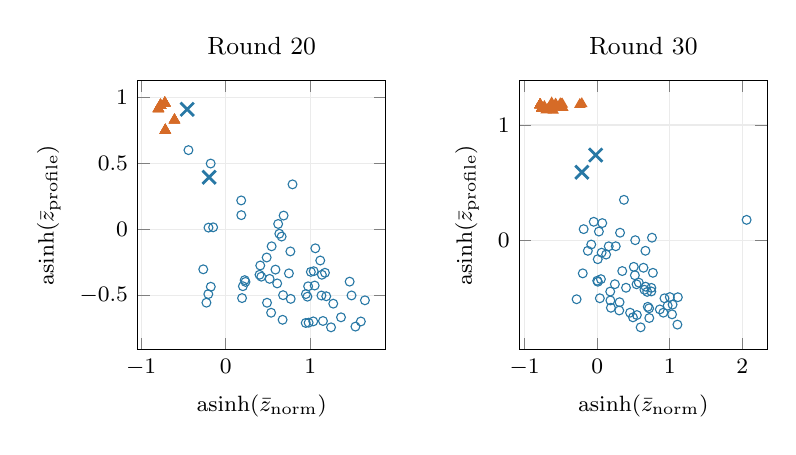
\begin{tikzpicture}
\begin{groupplot}[group style={group size=2 by 1,horizontal sep=1.7cm},width=.39\textwidth,height=5cm,grid=major,grid style={black!8},xlabel={$\operatorname{asinh}(\bar z_{\rm norm})$},ylabel={$\operatorname{asinh}(\bar z_{\rm profile})$},tick label style={font=\footnotesize},label style={font=\footnotesize},title style={font=\small},unbounded coords=jump]
\nextgroupplot[title={Round 20}]
\addplot[only marks,mark=o,mark size=1.6pt,draw=honestblue] table[x=x,y=y,row sep=\\] {% PLOT DATA: generated/revision/error_honest_20.dat (58 data rows)
x y \\
1.007452495056477 -0.3235179208990485 \\
0.489201235052194 -0.5575668632622613 \\
0.22513767275665647 -0.38614712142719687 \\
0.7654394556511567 -0.16847871628052116 \\
0.7694113055549335 -0.5281487778259716 \\
0.6346595468741965 -0.03428331145940987 \\
1.0359593177693067 -0.6990161919096349 \\
1.0603796751929457 -0.14490405003881482 \\
0.9752294164333228 -0.4328340854974942 \\
1.5345958608500554 -0.7382965187319586 \\
0.589039384198732 -0.30622113629729647 \\
-0.1756072803260052 -0.436222957576851 \\
0.9468272551059284 -0.7106542057772947 \\
1.2459655555142901 -0.7438686755243418 \\
0.7481601159610972 -0.3348971881468389 \\
0.609674448116855 -0.4111295735591068 \\
1.3639291402586913 -0.6679279572354708 \\
0.40055168038613154 -0.34530836740885834 \\
-0.17711574565627922 0.4977785485784197 \\
0.5198801990467745 -0.37641250986134034 \\
0.7906872792552958 0.33984925776230573 \\
0.4848565905035588 -0.2144763384478094 \\
0.19394924750302847 -0.5221116967516978 \\
0.5436566412839277 -0.12969805780294452 \\
1.1744215987582047 -0.33027842595407014 \\
1.2722704373551934 -0.5644950247342214 \\
-0.2645431361197029 -0.3040527178594838 \\
-0.14796752730576115 0.014439961988263845 \\
0.6209674817263958 0.03978513330557131 \\
0.20395534837250273 -0.43223727047265237 \\
1.132853210351763 -0.5026885178594007 \\
0.18406683214512623 0.21807643863510529 \\
0.40925867409687444 -0.27523375290945606 \\
-0.2048104960030042 -0.4919359883985535 \\
1.0409741722606394 -0.3183821363231651 \\
0.9671724947679846 -0.511574752473202 \\
1.1380902985656376 -0.34534586780018456 \\
1.5985870027088986 -0.6995163829091149 \\
-0.2270779457497603 -0.5570586110605498 \\
0.6733539493385495 -0.6867024901004075 \\
0.6618616755766132 -0.05576748702092196 \\
1.6468649168979037 -0.5390355126190196 \\
1.189283822293529 -0.5084136145198092 \\
0.9491664512697205 -0.49164378423129235 \\
0.6852731348783109 0.10327242304489162 \\
0.9810982661481277 -0.7087686798184412 \\
1.0525386356232247 -0.42701741111692465 \\
1.4882049727543971 -0.5021521215999831 \\
1.1186283467168103 -0.23730208430337651 \\
1.466057960310782 -0.3974592193113427 \\
0.4217055188363508 -0.35987654830785726 \\
1.1505544029481989 -0.6957701907615038 \\
-0.20270360950830835 0.01203905991710798 \\
0.23455922436189827 -0.3993596001694787 \\
0.5375907034926437 -0.6332255523053789 \\
0.18493296206656576 0.10656264210735812 \\
-0.43954001570822887 0.5994015785168101 \\
0.6790952198862802 -0.5000914388487644 \\
};
\addplot[only marks,mark=triangle*,mark size=2pt,draw=riderorange,fill=riderorange] table[x=x,y=y,row sep=\\] {% PLOT DATA: generated/revision/error_rider_20.dat (40 data rows)
x y \\
-0.7699415543491865 0.9400658052167656 \\
-0.7699415543491865 0.9400658052167656 \\
-0.71870721752817 0.9565907505775193 \\
-0.7947531840576698 0.9134921452018818 \\
-0.7138194132834639 0.749521611736949 \\
-0.6048253050878466 0.8273627143203383 \\
-0.7699415543491865 0.9400658052167656 \\
-0.6048253050878466 0.8273627143203383 \\
-0.7138194132834639 0.749521611736949 \\
-0.7138194132834639 0.749521611736949 \\
-0.6048253050878466 0.8273627143203383 \\
-0.7699415543491865 0.9400658052167656 \\
-0.71870721752817 0.9565907505775193 \\
-0.7138194132834639 0.749521611736949 \\
-0.7699415543491865 0.9400658052167656 \\
-0.7699415543491865 0.9400658052167656 \\
-0.7138194132834639 0.749521611736949 \\
-0.7947531840576698 0.9134921452018818 \\
-0.71870721752817 0.9565907505775193 \\
-0.6048253050878466 0.8273627143203383 \\
-0.6048253050878466 0.8273627143203383 \\
-0.7699415543491865 0.9400658052167656 \\
-0.7947531840576698 0.9134921452018818 \\
-0.7699415543491865 0.9400658052167656 \\
-0.6048253050878466 0.8273627143203383 \\
-0.7138194132834639 0.749521611736949 \\
-0.7138194132834639 0.749521611736949 \\
-0.71870721752817 0.9565907505775193 \\
-0.7138194132834639 0.749521611736949 \\
-0.71870721752817 0.9565907505775193 \\
-0.71870721752817 0.9565907505775193 \\
-0.7138194132834639 0.749521611736949 \\
-0.7947531840576698 0.9134921452018818 \\
-0.71870721752817 0.9565907505775193 \\
-0.7947531840576698 0.9134921452018818 \\
-0.7947531840576698 0.9134921452018818 \\
-0.7699415543491865 0.9400658052167656 \\
-0.7138194132834639 0.749521611736949 \\
-0.71870721752817 0.9565907505775193 \\
-0.71870721752817 0.9565907505775193 \\
};
\addplot[only marks,mark=x,mark size=3.4pt,line width=1pt,draw=honestblue] table[x=x,y=y,row sep=\\] {% PLOT DATA: generated/revision/error_error_20.dat (2 data rows)
x y \\
-0.19511120745870333 0.39343611761311925 \\
-0.45461766601386233 0.909049927667586 \\
};
\nextgroupplot[title={Round 30}]
\addplot[only marks,mark=o,mark size=1.6pt,draw=honestblue] table[x=x,y=y,row sep=\\] {% PLOT DATA: generated/revision/error_honest_30.dat (58 data rows)
x y \\
0.7184125725417797 -0.6708174706785802 \\
0.18255308083116864 -0.5187473854962943 \\
0.008059084611330777 -0.16169319223059958 \\
0.6653628937046563 -0.08881054661676333 \\
0.5247057735443948 0.002783602982985151 \\
0.345776761104023 -0.2643390013938472 \\
0.5991453159858081 -0.7515032507368683 \\
0.7555561780007662 0.0244313130340511 \\
0.6516351345085966 -0.4263390299057761 \\
1.0392602187772089 -0.5548384474032421 \\
0.31552224202790924 0.06757013982634374 \\
-0.08124826528696519 -0.03465820610394273 \\
0.4538561062743678 -0.6249532086274843 \\
0.6974005277481309 -0.573850293760915 \\
0.397747606515093 -0.40887781125188005 \\
0.25634523271082316 -0.04948863478316996 \\
0.9717244552496093 -0.5640648724124231 \\
0.189446592952823 -0.5821679448743925 \\
0.06146848642003584 -0.1051568763335212 \\
0.5197624742366483 -0.30068963183300507 \\
0.5739467282176365 -0.3644240704704003 \\
0.36934123022539467 0.35229058702215904 \\
0.010044233646871254 -0.35679052652759224 \\
0.1803198874178202 -0.44190382347060525 \\
0.6676390895210317 -0.3996847339458145 \\
0.7681443579276382 -0.2795456161023739 \\
-0.18602050721215205 0.09857144023471663 \\
0.0240953669705266 0.07776968264357881 \\
0.8636981990883095 -0.5965240165088153 \\
0.0009898577617452329 -0.3480446173063134 \\
0.9120723591013343 -0.6246649847580551 \\
0.15947018701770913 -0.049841893370049455 \\
0.05162099638197081 -0.33453708660452686 \\
-0.19844611863995207 -0.28423935279837426 \\
0.6383691594854629 -0.2357157287434055 \\
0.5476252644669575 -0.6453066742665925 \\
0.7468245412757684 -0.4409373728718541 \\
1.106154767222361 -0.7279642668406218 \\
-0.2832221022544682 -0.5084553000337774 \\
0.3047557182772692 -0.6055041160332152 \\
0.5047247493212826 -0.22781232306941795 \\
1.0323020027019867 -0.6390768460659174 \\
0.9278487447427957 -0.5001052473038721 \\
1.1122397629009046 -0.4909111818256106 \\
0.5426590847140647 -0.3788776463473816 \\
0.49332167898948764 -0.6650199372830662 \\
0.7471717759633064 -0.4100234875880356 \\
1.0012696752946462 -0.48964200124767276 \\
0.716143576019847 -0.5868965386391082 \\
2.0599674890515387 0.17887971810327213 \\
0.07034335581103955 0.151040835740418 \\
0.6901258719762418 -0.44467033590937544 \\
-0.1286284730773505 -0.08898979943384214 \\
0.036998041871289855 -0.4999124973155467 \\
0.24407363950943242 -0.37811094663100203 \\
-0.04723681929348483 0.16232451708357803 \\
0.12336715488541693 -0.12140196139438114 \\
0.3088639740051826 -0.5340972062447422 \\
};
\addplot[only marks,mark=triangle*,mark size=2pt,draw=riderorange,fill=riderorange] table[x=x,y=y,row sep=\\] {% PLOT DATA: generated/revision/error_rider_30.dat (40 data rows)
x y \\
-0.7633092435062286 1.144467544071806 \\
-0.7864562673320539 1.1748573620029938 \\
-0.6028801931727138 1.1573426367336501 \\
-0.5081804444664733 1.1647941836012778 \\
-0.7864562673320539 1.1748573620029938 \\
-0.4801888210370803 1.180126526183217 \\
-0.7864562673320539 1.1748573620029938 \\
-0.7864562673320539 1.1748573620029938 \\
-0.7633092435062286 1.144467544071806 \\
-0.7633092435062286 1.144467544071806 \\
-0.7864562673320539 1.1748573620029938 \\
-0.5102672902328748 1.1809002138239002 \\
-0.7864562673320539 1.1748573620029938 \\
-0.49285761279675483 1.1777473153398406 \\
-0.6688021294517494 1.1424733506646836 \\
-0.7036290707525459 1.1293908215883492 \\
-0.2386264435988342 1.177629495571546 \\
-0.5012250272426262 1.1824002137774623 \\
-0.72765936515038 1.1601532536609784 \\
-0.7864562673320539 1.1748573620029938 \\
-0.7864562673320539 1.1748573620029938 \\
-0.7864562673320539 1.1748573620029938 \\
-0.47406775196266543 1.1522006224865429 \\
-0.6056069116268251 1.127372013002761 \\
-0.2113560112515184 1.1837540497455585 \\
-0.7633092435062286 1.144467544071806 \\
-0.7633092435062286 1.144467544071806 \\
-0.7864562673320539 1.1748573620029938 \\
-0.5670370643117467 1.1747392605474387 \\
-0.6688021294517494 1.1424733506646836 \\
-0.7633092435062286 1.144467544071806 \\
-0.7633092435062286 1.144467544071806 \\
-0.7864562673320539 1.1748573620029938 \\
-0.6688021294517494 1.1424733506646836 \\
-0.7864562673320539 1.1748573620029938 \\
-0.5746597923899034 1.179442492424577 \\
-0.7864562673320539 1.1748573620029938 \\
-0.6268159553490236 1.190566630440373 \\
-0.7864562673320539 1.1748573620029938 \\
-0.7864562673320539 1.1748573620029938 \\
};
\addplot[only marks,mark=x,mark size=3.4pt,line width=1pt,draw=honestblue] table[x=x,y=y,row sep=\\] {% PLOT DATA: generated/revision/error_error_30.dat (2 data rows)
x y \\
-0.020115842860335884 0.739675124500126 \\
-0.21053346715466092 0.5913127294265466 \\
};
\end{groupplot}\end{tikzpicture}
\par\smallskip{\footnotesize\textcolor{honestblue}{$\circ$} Honest\quad\textcolor{riderorange}{$\blacktriangle$} Free rider\quad\textcolor{honestblue}{$\times$} Honest client removed at round 30}
\caption{A recorded honest-client error case. MNIST non-IID FR3, 40\% free riders, study seed 43. Each point averages selected A/B scores. Crosses mark the two honest clients removed by repeated profile certificates. Points can coincide.}\label{fig:honest-error}
\end{figure*}

% END SOURCE: generated/revision/honest_error_figure.tex


The tested fabrications also have favorable magnitude structure. FR1
has zero delta, FR2 uses small fixed noise, and FR3--FR4 recycle shared
model changes. Averaging does not mathematically guarantee a smaller norm
in every trajectory, but the displayed cases are strongly low-norm.
Their results therefore cannot establish robustness to a norm-matched
adversary or isolate the profile score's incremental value.

\subsection{Oracle Norm-Matching Feature Diagnostic}
To isolate that limitation, we replay each initial FR2--FR4 pair from the
96-run study: 72 cases across both datasets, partitions, proportions and
the three study seeds. The unchanged detector must reproduce every
stored round-20 certificate before stress testing. We then replace each
free rider's norm by the same-trap median honest norm. Positive rescaling
preserves the normalized profile in~\eqref{eq:profile}; profiles are held
fixed and the peer scores and certificates are recomputed.

Evaluation labels construct this oracle stress input; they are not given
to the detector. This provides the adversary extra information and
operates on stored features rather than newly fabricated full models.
It tests statistical certificates at one complete cycle, not confirmed
removal, adaptation or model utility. FR1 is excluded because a zero
vector cannot be positively rescaled to a nonzero norm.

% BEGIN SOURCE: generated/revision/norm_matching_table.tex
\begin{table*}[t]\centering\footnotesize\setlength{\tabcolsep}{4pt}
\caption{Round-20 statistical certificates under oracle norm matching.}\label{tab:norm-matching}
\begin{tabular}{lrrrrrr}\toprule
& \multicolumn{3}{c}{Stored responses: attacker certificates (\%)} & \multicolumn{3}{c}{Norm matched} \\
\cmidrule(lr){2-4}\cmidrule(lr){5-7}
Attack & Norm & Profile & Either & Norm (\%) & Profile/either (\%) & Honest certificates \\ \midrule
FR2 & 100.0 & 100.0 & 100.0 & 0.0 & 61.9 & 5 \\
FR3 & 38.1 & 50.0 & 79.8 & 0.0 & 10.7 & 2 \\
FR4 & 78.6 & 34.5 & 82.1 & 0.0 & 17.9 & 3 \\
\bottomrule\end{tabular}
\par\smallskip\parbox{.96\textwidth}{\scriptsize Each attack row covers 24 federations, 840 attacker client-cases and 1,560 honest client-cases across both datasets, partitions, 30\%/40\% and three seeds. Rates pool attacker certificates; honest entries are counts. Norm matching uses an oracle honest median and keeps scale-free profiles fixed. The endpoint is one paired statistical certificate, not removal.}
\end{table*}

% END SOURCE: generated/revision/norm_matching_table.tex

The low-norm channel certifies no attackers after norm matching.
Profile certificates retain 61.9\% coverage for FR2, but only 10.7\%
for FR3 and 17.9\% for FR4, with ten honest certificates across the
stress cases. Profiles therefore supply some magnitude-independent
evidence, while leaving a substantial detection gap. Whether these
certificates would recur and confirm removal is unobserved here.
Both channels retain the joint nomination step. These are certificate
breakdowns within the unchanged pipeline, not comparisons of separate
norm-only and profile-only detectors.

\subsection{Honest-Only and Lower-Prevalence Checks}
The prospective review engine freezes the v15.4 statistical settings and
corrects only the audit-clock liveness guard. Four honest-only 100-round
runs cover both datasets and both partitions with seed 42. None removes
an honest client. This is evidence from four federations, not a population
false-positive guarantee.

Table~\ref{tab:low-share} reports the complete non-IID 5\%, 10\% and
20\% grid available at this revision. FR1 removes all free riders at each
share. FR2--FR4 remove none at 5\%, while the completed 10\% and 20\%
cases remove all. The cohort-support requirement in~\eqref{eq:cohort-support}
is ten at 100 active clients, making a five-client statistical cohort
ineligible. This limit is retained rather than relaxed after observing
misses. CIFAR-10 FR3 at 10\% also removes one honest client.

% BEGIN SOURCE: generated/revision/low_share_table.tex
\begin{table}[t]\centering\footnotesize\setlength{\tabcolsep}{3.5pt}
\caption{Completed non-IID lower-prevalence checks.}\label{tab:low-share}
\begin{tabular}{lrrrrr}\toprule
Dataset & FR (\%) & FR1 & FR2 & FR3 & FR4 \\ \midrule
MNIST & 5 & 5/5 & 0/5 & 0/5 & 0/5 \\
MNIST & 10 & 10/10 & 10/10 & 10/10 & 10/10 \\
MNIST & 20 & 20/20 & 20/20 & 20/20 & 20/20 \\
\midrule
CIFAR-10 & 5 & 5/5 & 0/5 & 0/5 & 0/5 \\
CIFAR-10 & 10 & 10/10 & 10/10 & 10/10$^{\dagger}$ & 10/10 \\
CIFAR-10 & 20 & 20/20 & 20/20 & 20/20 & 20/20 \\
\bottomrule\end{tabular}
\par\smallskip\parbox{\columnwidth}{\scriptsize Entries are free riders permanently removed / present by round 100. One frozen seed, 100 clients per run. $\dagger$ One honest removal; all other displayed runs have none.}
\end{table}

% END SOURCE: generated/revision/low_share_table.tex


At the evidence cutoff, 26 of 48 low-prevalence cases are complete,
including two IID MNIST 5\% cases where FR3 and FR4 remain undetected.
Passive ablation/MAD diagnostics, oracle utility comparisons, published
decaying-noise and scaled-delta tests, and the registered unseen-seed
phase are pending. They are not reported as completed evidence.

\subsection{Execution Time and Memory}
Table~\ref{tab:cost} reports multi-seed process measurements averaged over
the attacks, with minimum and maximum execution values in brackets.
Runs at 30\% free riders include more honest training jobs than those at
40\%, which helps explain their longer rounds. Process RSS includes
training tensors, simulated attacker histories and server state.
It should not be interpreted as detector-only memory.

The overall cost and the cost of the checking stages answer different
questions. Table~\ref{tab:cost} describes the complete simulation.
Section~\ref{sec:native-timing} measures selected operations, while
Section~\ref{sec:complexity} analyzes their scaling.

% BEGIN SOURCE: generated/cost.tex
\begin{table*}[t]
\centering\footnotesize\setlength{\tabcolsep}{4pt}
\caption{Execution time and process memory.}\label{tab:cost}
\begin{tabular}{llrrrr}
\toprule
Dataset & Partition & FR (\%) & \shortstack{Round time (s)\\mean [range]} & \shortstack{Peak process RSS (GiB)\\mean [range]} & \shortstack{Execution duration\\(min/run)} \\
\midrule
\multirow{4}{*}{MNIST} & \multirow{2}{*}{IID} & 30 & 42.38 [39.78--48.57] & 0.54 [0.29--0.78] & 75.02 \\
 &  & 40 & 37.05 [35.35--42.68] & 0.60 [0.30--0.88] & 66.71 \\
 & \multirow{2}{*}{Non-IID} & 30 & 41.62 [40.57--43.43] & 0.57 [0.30--0.78] & 73.79 \\
 &  & 40 & 36.08 [34.34--38.67] & 0.62 [0.30--0.88] & 65.27 \\
\midrule
\multirow{4}{*}{CIFAR-10} & \multirow{2}{*}{IID} & 30 & 99.35 [88.18--119.07] & 1.24 [0.70--1.76] & 175.07 \\
 &  & 40 & 85.35 [73.52--104.21] & 1.38 [0.71--2.06] & 154.65 \\
 & \multirow{2}{*}{Non-IID} & 30 & 92.30 [82.85--108.38] & 1.31 [0.73--1.79] & 161.97 \\
 &  & 40 & 77.03 [69.10--84.85] & 1.49 [0.75--2.14] & 139.40 \\
\bottomrule
\end{tabular}
\end{table*}

% END SOURCE: generated/cost.tex


\subsection{Comparison with No-Defense Federated Averaging}\label{sec:baseline}
The no-defense baseline keeps all clients throughout training and
aggregates every response. It performs no traps, screening, quarantine
or removal. Each completed baseline is matched to BaitFL using the same
dataset, partition, attack, proportion and random seed. Configuration
checks and identical warmup accuracies verify that the paired runs start
from the same training conditions.

Table~\ref{tab:baseline} uses 81 completed matched
runs: 33 on MNIST and
48 on CIFAR-10. Means are calculated across matched seeds within
each attack, then across the four attacks with equal weight. A BaitFL
execution without a completed baseline partner does not enter this
comparison, even though it remains in Table~\ref{tab:performance}.
Positive accuracy changes favor BaitFL. A positive time change means
longer rounds. Accuracy differences are expressed in percentage points.

The available paired means show comparable or slightly higher final
accuracy with BaitFL. Their descriptive mean differences are
0.08 percentage points on MNIST and 0.61
on CIFAR-10, with variation across attacks and partitions. MNIST baseline
coverage remains uneven, while CIFAR-10 now covers the complete matched
grid. These differences do not establish a systematic accuracy gain
across random seeds. That assessment requires paired differences with
uncertainty estimates from more complete replication coverage.
MNIST rounds become modestly shorter, while the current CIFAR-10
comparisons take somewhat longer than no defense. These are whole-workflow
measurements of the full training procedure. Stage-level timing is
examined separately below.

% BEGIN SOURCE: generated/baseline_table.tex
\begin{table*}[t]\centering\footnotesize\setlength{\tabcolsep}{5pt}
\caption{Comparison with no-defense aggregation.}\label{tab:baseline}
\begin{tabular}{llrrrrrrr}\toprule
\multirow{2}{*}{Dataset} & \multirow{2}{*}{Partition} & \multirow{2}{*}{FR (\%)} & \multicolumn{3}{c}{Final accuracy (\%)} & \multicolumn{3}{c}{Mean round time (s)} \\
\cmidrule(lr){4-6}\cmidrule(lr){7-9}
& & & No defense & BaitFL & \shortstack{Difference\\(percentage points)} & No defense & BaitFL & Change (\%) \\ \midrule
\multirow{4}{*}{MNIST} & \multirow{2}{*}{IID} & 30 & 98.92 & 98.99 & +0.07 & 44.49 & 41.64 & -6.39 \\
 &  & 40 & 98.82 & 98.91 & +0.09 & 38.10 & 36.96 & -3.01 \\
\cmidrule(lr){2-9}
 & \multirow{2}{*}{Non-IID} & 30 & 98.91 & 98.94 & +0.03 & 45.46 & 41.44 & -8.84 \\
 &  & 40 & 98.79 & 98.93 & +0.14 & 37.35 & 35.50 & -4.96 \\
\midrule
\multirow{4}{*}{CIFAR-10} & \multirow{2}{*}{IID} & 30 & 77.37 & 77.80 & +0.44 & 94.90 & 99.35 & +4.68 \\
 &  & 40 & 76.31 & 77.02 & +0.71 & 81.28 & 85.35 & +5.01 \\
\cmidrule(lr){2-9}
 & \multirow{2}{*}{Non-IID} & 30 & 75.35 & 75.84 & +0.49 & 91.28 & 92.30 & +1.12 \\
 &  & 40 & 73.90 & 74.69 & +0.79 & 74.52 & 77.03 & +3.37 \\
\bottomrule\end{tabular}\end{table*}

% END SOURCE: generated/baseline_table.tex


The observed accuracy differences describe the combined effect of detection and
mitigation. Removing fabricated responses changes aggregation, but
challenge rounds also withhold genuine updates. Final model utility
therefore depends on both effects, rather than on removal recall alone.

Figure~\ref{fig:accuracy-comparison} shows model accuracy from rounds
20--100, averaging all three BaitFL replications and the completed
no-defense runs. Baseline coverage is 2--3
replications per attack setting on MNIST and 3
on CIFAR-10. FR1--FR4 receive equal weight,
and each dataset row shares an accuracy scale. The curves show how
learning continues after initial challenge coverage. Coverage differs
between methods, so the paired accuracy differences in
Table~\ref{tab:baseline} remain the basis for the quantitative comparison.

% BEGIN SOURCE: generated/accuracy_comparison.tex
\begin{figure*}[!t]\centering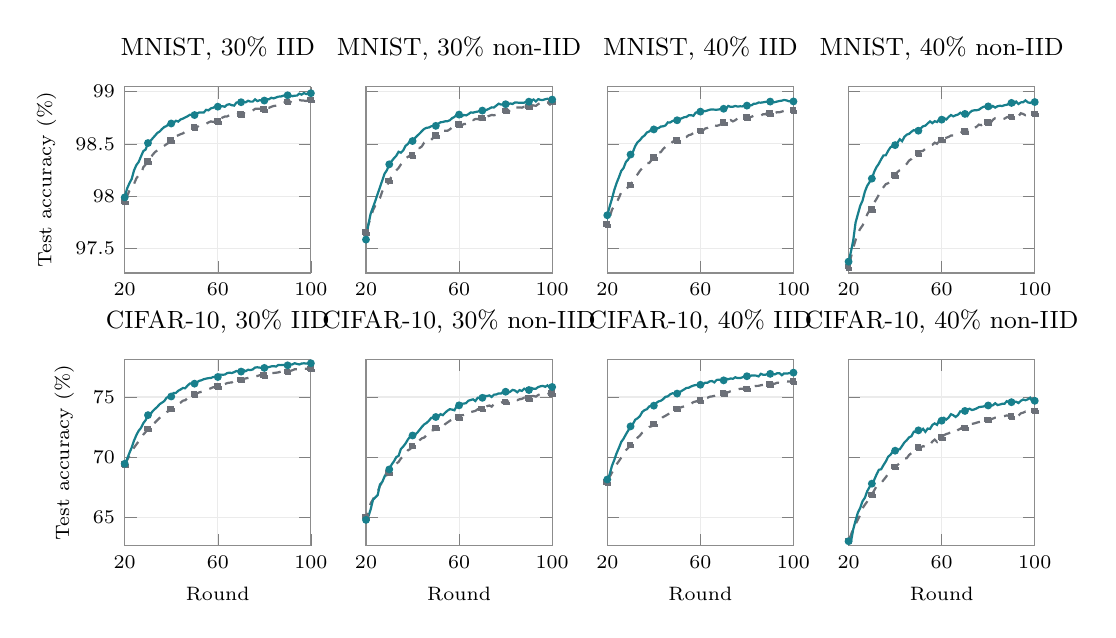
\begin{tikzpicture}
\begin{groupplot}[group style={group size=4 by 2,horizontal sep=0.7cm,vertical sep=1.1cm},scale only axis,width=0.195\textwidth,height=0.195\textwidth,xmin=20,xmax=100,xtick={20,60,100},grid=major,grid style={black!8},axis line style={black!45},tick label style={font=\scriptsize},title style={font=\small},label style={font=\scriptsize},scaled ticks=false,yticklabel style={/pgf/number format/fixed,/pgf/number format/precision=1}]
\nextgroupplot[title={MNIST, 30\% IID},ymin=97.26667,ymax=99.04583,ylabel={Test accuracy (\%)}]
\addplot[comparisongray,dashed,thick,mark=square*,mark size=1pt,mark repeat=10] table[col sep=comma,x=round,y=accuracy,row sep=\\] {% PLOT DATA: generated/comparison/accuracy_all_baseline_mnist_iid_30.csv (100 data rows)
method,dataset,split,share,round,accuracy,minimum_replications,maximum_replications \\
baseline,mnist,iid,30,1,87.38874999999999,2,2 \\
baseline,mnist,iid,30,2,92.2225,2,2 \\
baseline,mnist,iid,30,3,93.95625,2,2 \\
baseline,mnist,iid,30,4,94.92374999999998,2,2 \\
baseline,mnist,iid,30,5,95.47375,2,2 \\
baseline,mnist,iid,30,6,95.90875000000001,2,2 \\
baseline,mnist,iid,30,7,96.2525,2,2 \\
baseline,mnist,iid,30,8,96.53625,2,2 \\
baseline,mnist,iid,30,9,96.8025,2,2 \\
baseline,mnist,iid,30,10,97.01125,2,2 \\
baseline,mnist,iid,30,11,97.14375,2,2 \\
baseline,mnist,iid,30,12,97.27,2,2 \\
baseline,mnist,iid,30,13,97.39125,2,2 \\
baseline,mnist,iid,30,14,97.52,2,2 \\
baseline,mnist,iid,30,15,97.5975,2,2 \\
baseline,mnist,iid,30,16,97.6875,2,2 \\
baseline,mnist,iid,30,17,97.775,2,2 \\
baseline,mnist,iid,30,18,97.84625,2,2 \\
baseline,mnist,iid,30,19,97.89625000000001,2,2 \\
baseline,mnist,iid,30,20,97.9525,2,2 \\
baseline,mnist,iid,30,21,97.99874999999999,2,2 \\
baseline,mnist,iid,30,22,98.0525,2,2 \\
baseline,mnist,iid,30,23,98.08625,2,2 \\
baseline,mnist,iid,30,24,98.11625000000001,2,2 \\
baseline,mnist,iid,30,25,98.17125000000001,2,2 \\
baseline,mnist,iid,30,26,98.19999999999999,2,2 \\
baseline,mnist,iid,30,27,98.20874999999998,2,2 \\
baseline,mnist,iid,30,28,98.2775,2,2 \\
baseline,mnist,iid,30,29,98.30375,2,2 \\
baseline,mnist,iid,30,30,98.3375,2,2 \\
baseline,mnist,iid,30,31,98.35875,2,2 \\
baseline,mnist,iid,30,32,98.39625,2,2 \\
baseline,mnist,iid,30,33,98.42124999999999,2,2 \\
baseline,mnist,iid,30,34,98.43875,2,2 \\
baseline,mnist,iid,30,35,98.44625,2,2 \\
baseline,mnist,iid,30,36,98.47,2,2 \\
baseline,mnist,iid,30,37,98.48249999999999,2,2 \\
baseline,mnist,iid,30,38,98.49750000000002,2,2 \\
baseline,mnist,iid,30,39,98.51249999999999,2,2 \\
baseline,mnist,iid,30,40,98.53875,2,2 \\
baseline,mnist,iid,30,41,98.55375,2,2 \\
baseline,mnist,iid,30,42,98.575,2,2 \\
baseline,mnist,iid,30,43,98.5825,2,2 \\
baseline,mnist,iid,30,44,98.5925,2,2 \\
baseline,mnist,iid,30,45,98.6,2,2 \\
baseline,mnist,iid,30,46,98.61625000000001,2,2 \\
baseline,mnist,iid,30,47,98.61875,2,2 \\
baseline,mnist,iid,30,48,98.62625,2,2 \\
baseline,mnist,iid,30,49,98.64875,2,2 \\
baseline,mnist,iid,30,50,98.66250000000001,2,2 \\
baseline,mnist,iid,30,51,98.65875,2,2 \\
baseline,mnist,iid,30,52,98.6775,2,2 \\
baseline,mnist,iid,30,53,98.68375,2,2 \\
baseline,mnist,iid,30,54,98.69125,2,2 \\
baseline,mnist,iid,30,55,98.6925,2,2 \\
baseline,mnist,iid,30,56,98.705,2,2 \\
baseline,mnist,iid,30,57,98.715,2,2 \\
baseline,mnist,iid,30,58,98.70999999999998,2,2 \\
baseline,mnist,iid,30,59,98.715,2,2 \\
baseline,mnist,iid,30,60,98.72125,2,2 \\
baseline,mnist,iid,30,61,98.7425,2,2 \\
baseline,mnist,iid,30,62,98.75125,2,2 \\
baseline,mnist,iid,30,63,98.76125,2,2 \\
baseline,mnist,iid,30,64,98.7625,2,2 \\
baseline,mnist,iid,30,65,98.77375,2,2 \\
baseline,mnist,iid,30,66,98.77624999999999,2,2 \\
baseline,mnist,iid,30,67,98.77125,2,2 \\
baseline,mnist,iid,30,68,98.77875,2,2 \\
baseline,mnist,iid,30,69,98.78875,2,2 \\
baseline,mnist,iid,30,70,98.78375,2,2 \\
baseline,mnist,iid,30,71,98.79375,2,2 \\
baseline,mnist,iid,30,72,98.7925,2,2 \\
baseline,mnist,iid,30,73,98.79875,2,2 \\
baseline,mnist,iid,30,74,98.80624999999999,2,2 \\
baseline,mnist,iid,30,75,98.8175,2,2 \\
baseline,mnist,iid,30,76,98.83500000000001,2,2 \\
baseline,mnist,iid,30,77,98.83624999999999,2,2 \\
baseline,mnist,iid,30,78,98.83500000000001,2,2 \\
baseline,mnist,iid,30,79,98.83999999999999,2,2 \\
baseline,mnist,iid,30,80,98.83250000000001,2,2 \\
baseline,mnist,iid,30,81,98.84375,2,2 \\
baseline,mnist,iid,30,82,98.845,2,2 \\
baseline,mnist,iid,30,83,98.85499999999999,2,2 \\
baseline,mnist,iid,30,84,98.8625,2,2 \\
baseline,mnist,iid,30,85,98.865,2,2 \\
baseline,mnist,iid,30,86,98.86625000000001,2,2 \\
baseline,mnist,iid,30,87,98.87375,2,2 \\
baseline,mnist,iid,30,88,98.88624999999999,2,2 \\
baseline,mnist,iid,30,89,98.9025,2,2 \\
baseline,mnist,iid,30,90,98.905,2,2 \\
baseline,mnist,iid,30,91,98.905,2,2 \\
baseline,mnist,iid,30,92,98.89250000000001,2,2 \\
baseline,mnist,iid,30,93,98.89750000000001,2,2 \\
baseline,mnist,iid,30,94,98.90875,2,2 \\
baseline,mnist,iid,30,95,98.92,2,2 \\
baseline,mnist,iid,30,96,98.915,2,2 \\
baseline,mnist,iid,30,97,98.91375000000001,2,2 \\
baseline,mnist,iid,30,98,98.91000000000001,2,2 \\
baseline,mnist,iid,30,99,98.91875,2,2 \\
baseline,mnist,iid,30,100,98.92374999999998,2,2 \\
};
\addplot[baitteal,thick,mark=*,mark size=1pt,mark repeat=10] table[col sep=comma,x=round,y=accuracy,row sep=\\] {% PLOT DATA: generated/comparison/accuracy_all_bait_mnist_iid_30.csv (100 data rows)
method,dataset,split,share,round,accuracy,minimum_replications,maximum_replications \\
bait,mnist,iid,30,1,87.38666666666667,3,3 \\
bait,mnist,iid,30,2,92.03583333333331,3,3 \\
bait,mnist,iid,30,3,93.82833333333335,3,3 \\
bait,mnist,iid,30,4,94.78416666666666,3,3 \\
bait,mnist,iid,30,5,95.37833333333333,3,3 \\
bait,mnist,iid,30,6,95.81916666666667,3,3 \\
bait,mnist,iid,30,7,96.19916666666667,3,3 \\
bait,mnist,iid,30,8,96.49333333333333,3,3 \\
bait,mnist,iid,30,9,96.75916666666666,3,3 \\
bait,mnist,iid,30,10,96.97833333333332,3,3 \\
bait,mnist,iid,30,11,97.1225,3,3 \\
bait,mnist,iid,30,12,97.255,3,3 \\
bait,mnist,iid,30,13,97.38666666666667,3,3 \\
bait,mnist,iid,30,14,97.51249999999999,3,3 \\
bait,mnist,iid,30,15,97.60666666666667,3,3 \\
bait,mnist,iid,30,16,97.695,3,3 \\
bait,mnist,iid,30,17,97.76083333333334,3,3 \\
bait,mnist,iid,30,18,97.82166666666666,3,3 \\
bait,mnist,iid,30,19,97.8575,3,3 \\
bait,mnist,iid,30,20,97.98916666666668,3,3 \\
bait,mnist,iid,30,21,98.0725,3,3 \\
bait,mnist,iid,30,22,98.12333333333333,3,3 \\
bait,mnist,iid,30,23,98.165,3,3 \\
bait,mnist,iid,30,24,98.24666666666667,3,3 \\
bait,mnist,iid,30,25,98.2975,3,3 \\
bait,mnist,iid,30,26,98.32750000000001,3,3 \\
bait,mnist,iid,30,27,98.38083333333333,3,3 \\
bait,mnist,iid,30,28,98.43166666666667,3,3 \\
bait,mnist,iid,30,29,98.44666666666666,3,3 \\
bait,mnist,iid,30,30,98.50833333333333,3,3 \\
bait,mnist,iid,30,31,98.52666666666667,3,3 \\
bait,mnist,iid,30,32,98.55333333333334,3,3 \\
bait,mnist,iid,30,33,98.57833333333333,3,3 \\
bait,mnist,iid,30,34,98.60416666666667,3,3 \\
bait,mnist,iid,30,35,98.61833333333334,3,3 \\
bait,mnist,iid,30,36,98.64166666666665,3,3 \\
bait,mnist,iid,30,37,98.66166666666668,3,3 \\
bait,mnist,iid,30,38,98.67083333333333,3,3 \\
bait,mnist,iid,30,39,98.69500000000001,3,3 \\
bait,mnist,iid,30,40,98.69500000000001,3,3 \\
bait,mnist,iid,30,41,98.7025,3,3 \\
bait,mnist,iid,30,42,98.72083333333333,3,3 \\
bait,mnist,iid,30,43,98.71333333333332,3,3 \\
bait,mnist,iid,30,44,98.73333333333333,3,3 \\
bait,mnist,iid,30,45,98.74166666666667,3,3 \\
bait,mnist,iid,30,46,98.75333333333333,3,3 \\
bait,mnist,iid,30,47,98.76416666666665,3,3 \\
bait,mnist,iid,30,48,98.77833333333334,3,3 \\
bait,mnist,iid,30,49,98.77583333333334,3,3 \\
bait,mnist,iid,30,50,98.77583333333334,3,3 \\
bait,mnist,iid,30,51,98.79083333333334,3,3 \\
bait,mnist,iid,30,52,98.8,3,3 \\
bait,mnist,iid,30,53,98.80083333333333,3,3 \\
bait,mnist,iid,30,54,98.80083333333333,3,3 \\
bait,mnist,iid,30,55,98.82583333333332,3,3 \\
bait,mnist,iid,30,56,98.82083333333333,3,3 \\
bait,mnist,iid,30,57,98.83916666666664,3,3 \\
bait,mnist,iid,30,58,98.84583333333333,3,3 \\
bait,mnist,iid,30,59,98.85583333333332,3,3 \\
bait,mnist,iid,30,60,98.85583333333332,3,3 \\
bait,mnist,iid,30,61,98.85666666666665,3,3 \\
bait,mnist,iid,30,62,98.86083333333333,3,3 \\
bait,mnist,iid,30,63,98.855,3,3 \\
bait,mnist,iid,30,64,98.87416666666667,3,3 \\
bait,mnist,iid,30,65,98.87916666666666,3,3 \\
bait,mnist,iid,30,66,98.87,3,3 \\
bait,mnist,iid,30,67,98.86583333333334,3,3 \\
bait,mnist,iid,30,68,98.89500000000001,3,3 \\
bait,mnist,iid,30,69,98.89833333333333,3,3 \\
bait,mnist,iid,30,70,98.89833333333333,3,3 \\
bait,mnist,iid,30,71,98.90333333333334,3,3 \\
bait,mnist,iid,30,72,98.8975,3,3 \\
bait,mnist,iid,30,73,98.9125,3,3 \\
bait,mnist,iid,30,74,98.90416666666667,3,3 \\
bait,mnist,iid,30,75,98.90416666666667,3,3 \\
bait,mnist,iid,30,76,98.92583333333334,3,3 \\
bait,mnist,iid,30,77,98.90916666666666,3,3 \\
bait,mnist,iid,30,78,98.91750000000002,3,3 \\
bait,mnist,iid,30,79,98.91416666666666,3,3 \\
bait,mnist,iid,30,80,98.91416666666666,3,3 \\
bait,mnist,iid,30,81,98.92666666666668,3,3 \\
bait,mnist,iid,30,82,98.92750000000001,3,3 \\
bait,mnist,iid,30,83,98.94083333333333,3,3 \\
bait,mnist,iid,30,84,98.935,3,3 \\
bait,mnist,iid,30,85,98.94333333333333,3,3 \\
bait,mnist,iid,30,86,98.95166666666665,3,3 \\
bait,mnist,iid,30,87,98.9525,3,3 \\
bait,mnist,iid,30,88,98.96000000000001,3,3 \\
bait,mnist,iid,30,89,98.96499999999999,3,3 \\
bait,mnist,iid,30,90,98.96499999999999,3,3 \\
bait,mnist,iid,30,91,98.96583333333334,3,3 \\
bait,mnist,iid,30,92,98.95583333333335,3,3 \\
bait,mnist,iid,30,93,98.96083333333334,3,3 \\
bait,mnist,iid,30,94,98.96166666666667,3,3 \\
bait,mnist,iid,30,95,98.97999999999999,3,3 \\
bait,mnist,iid,30,96,98.97083333333333,3,3 \\
bait,mnist,iid,30,97,98.98583333333332,3,3 \\
bait,mnist,iid,30,98,98.97666666666666,3,3 \\
bait,mnist,iid,30,99,98.98416666666667,3,3 \\
bait,mnist,iid,30,100,98.98416666666667,3,3 \\
};
\nextgroupplot[title={MNIST, 30\% non-IID},ymin=97.26667,ymax=99.04583,yticklabels=\empty]
\addplot[comparisongray,dashed,thick,mark=square*,mark size=1pt,mark repeat=10] table[col sep=comma,x=round,y=accuracy,row sep=\\] {% PLOT DATA: generated/comparison/accuracy_all_baseline_mnist_noniid_30.csv (100 data rows)
method,dataset,split,share,round,accuracy,minimum_replications,maximum_replications \\
baseline,mnist,noniid,30,1,81.06,2,2 \\
baseline,mnist,noniid,30,2,90.28375,2,2 \\
baseline,mnist,noniid,30,3,92.87500000000001,2,2 \\
baseline,mnist,noniid,30,4,94.09375,2,2 \\
baseline,mnist,noniid,30,5,94.8925,2,2 \\
baseline,mnist,noniid,30,6,95.31375,2,2 \\
baseline,mnist,noniid,30,7,95.70625,2,2 \\
baseline,mnist,noniid,30,8,96.07750000000001,2,2 \\
baseline,mnist,noniid,30,9,96.33875,2,2 \\
baseline,mnist,noniid,30,10,96.53999999999999,2,2 \\
baseline,mnist,noniid,30,11,96.72749999999999,2,2 \\
baseline,mnist,noniid,30,12,96.875,2,2 \\
baseline,mnist,noniid,30,13,97.0025,2,2 \\
baseline,mnist,noniid,30,14,97.1275,2,2 \\
baseline,mnist,noniid,30,15,97.24499999999999,2,2 \\
baseline,mnist,noniid,30,16,97.335,2,2 \\
baseline,mnist,noniid,30,17,97.42875000000001,2,2 \\
baseline,mnist,noniid,30,18,97.47625,2,2 \\
baseline,mnist,noniid,30,19,97.5925,2,2 \\
baseline,mnist,noniid,30,20,97.65625,2,2 \\
baseline,mnist,noniid,30,21,97.72625,2,2 \\
baseline,mnist,noniid,30,22,97.7925,2,2 \\
baseline,mnist,noniid,30,23,97.86625000000001,2,2 \\
baseline,mnist,noniid,30,24,97.9125,2,2 \\
baseline,mnist,noniid,30,25,97.95125,2,2 \\
baseline,mnist,noniid,30,26,97.98249999999999,2,2 \\
baseline,mnist,noniid,30,27,98.04625,2,2 \\
baseline,mnist,noniid,30,28,98.0925,2,2 \\
baseline,mnist,noniid,30,29,98.10000000000001,2,2 \\
baseline,mnist,noniid,30,30,98.15125,2,2 \\
baseline,mnist,noniid,30,31,98.19,2,2 \\
baseline,mnist,noniid,30,32,98.21625000000002,2,2 \\
baseline,mnist,noniid,30,33,98.24625,2,2 \\
baseline,mnist,noniid,30,34,98.27,2,2 \\
baseline,mnist,noniid,30,35,98.30375,2,2 \\
baseline,mnist,noniid,30,36,98.32624999999999,2,2 \\
baseline,mnist,noniid,30,37,98.36125,2,2 \\
baseline,mnist,noniid,30,38,98.37625,2,2 \\
baseline,mnist,noniid,30,39,98.39125,2,2 \\
baseline,mnist,noniid,30,40,98.39375,2,2 \\
baseline,mnist,noniid,30,41,98.42875000000001,2,2 \\
baseline,mnist,noniid,30,42,98.4625,2,2 \\
baseline,mnist,noniid,30,43,98.46,2,2 \\
baseline,mnist,noniid,30,44,98.47625,2,2 \\
baseline,mnist,noniid,30,45,98.5125,2,2 \\
baseline,mnist,noniid,30,46,98.5275,2,2 \\
baseline,mnist,noniid,30,47,98.52000000000001,2,2 \\
baseline,mnist,noniid,30,48,98.53875,2,2 \\
baseline,mnist,noniid,30,49,98.56125,2,2 \\
baseline,mnist,noniid,30,50,98.585,2,2 \\
baseline,mnist,noniid,30,51,98.58749999999999,2,2 \\
baseline,mnist,noniid,30,52,98.61625000000001,2,2 \\
baseline,mnist,noniid,30,53,98.625,2,2 \\
baseline,mnist,noniid,30,54,98.625,2,2 \\
baseline,mnist,noniid,30,55,98.625,2,2 \\
baseline,mnist,noniid,30,56,98.63875,2,2 \\
baseline,mnist,noniid,30,57,98.65625,2,2 \\
baseline,mnist,noniid,30,58,98.66875,2,2 \\
baseline,mnist,noniid,30,59,98.685,2,2 \\
baseline,mnist,noniid,30,60,98.69,2,2 \\
baseline,mnist,noniid,30,61,98.675,2,2 \\
baseline,mnist,noniid,30,62,98.69,2,2 \\
baseline,mnist,noniid,30,63,98.69125,2,2 \\
baseline,mnist,noniid,30,64,98.71000000000001,2,2 \\
baseline,mnist,noniid,30,65,98.73249999999999,2,2 \\
baseline,mnist,noniid,30,66,98.72749999999999,2,2 \\
baseline,mnist,noniid,30,67,98.7375,2,2 \\
baseline,mnist,noniid,30,68,98.7375,2,2 \\
baseline,mnist,noniid,30,69,98.72999999999999,2,2 \\
baseline,mnist,noniid,30,70,98.75375,2,2 \\
baseline,mnist,noniid,30,71,98.76124999999999,2,2 \\
baseline,mnist,noniid,30,72,98.76125,2,2 \\
baseline,mnist,noniid,30,73,98.76875,2,2 \\
baseline,mnist,noniid,30,74,98.77625,2,2 \\
baseline,mnist,noniid,30,75,98.77375,2,2 \\
baseline,mnist,noniid,30,76,98.77874999999999,2,2 \\
baseline,mnist,noniid,30,77,98.80250000000001,2,2 \\
baseline,mnist,noniid,30,78,98.81125,2,2 \\
baseline,mnist,noniid,30,79,98.8175,2,2 \\
baseline,mnist,noniid,30,80,98.81875,2,2 \\
baseline,mnist,noniid,30,81,98.825,2,2 \\
baseline,mnist,noniid,30,82,98.80375000000001,2,2 \\
baseline,mnist,noniid,30,83,98.825,2,2 \\
baseline,mnist,noniid,30,84,98.84625,2,2 \\
baseline,mnist,noniid,30,85,98.8475,2,2 \\
baseline,mnist,noniid,30,86,98.84875,2,2 \\
baseline,mnist,noniid,30,87,98.84625,2,2 \\
baseline,mnist,noniid,30,88,98.855,2,2 \\
baseline,mnist,noniid,30,89,98.85249999999999,2,2 \\
baseline,mnist,noniid,30,90,98.8575,2,2 \\
baseline,mnist,noniid,30,91,98.87375,2,2 \\
baseline,mnist,noniid,30,92,98.8675,2,2 \\
baseline,mnist,noniid,30,93,98.86375,2,2 \\
baseline,mnist,noniid,30,94,98.88000000000001,2,2 \\
baseline,mnist,noniid,30,95,98.89125,2,2 \\
baseline,mnist,noniid,30,96,98.88,2,2 \\
baseline,mnist,noniid,30,97,98.895,2,2 \\
baseline,mnist,noniid,30,98,98.89625,2,2 \\
baseline,mnist,noniid,30,99,98.87625,2,2 \\
baseline,mnist,noniid,30,100,98.9125,2,2 \\
};
\addplot[baitteal,thick,mark=*,mark size=1pt,mark repeat=10] table[col sep=comma,x=round,y=accuracy,row sep=\\] {% PLOT DATA: generated/comparison/accuracy_all_bait_mnist_noniid_30.csv (100 data rows)
method,dataset,split,share,round,accuracy,minimum_replications,maximum_replications \\
bait,mnist,noniid,30,1,81.43666666666667,3,3 \\
bait,mnist,noniid,30,2,90.00583333333333,3,3 \\
bait,mnist,noniid,30,3,92.67,3,3 \\
bait,mnist,noniid,30,4,93.91166666666668,3,3 \\
bait,mnist,noniid,30,5,94.71000000000001,3,3 \\
bait,mnist,noniid,30,6,95.155,3,3 \\
bait,mnist,noniid,30,7,95.555,3,3 \\
bait,mnist,noniid,30,8,95.92416666666668,3,3 \\
bait,mnist,noniid,30,9,96.19416666666666,3,3 \\
bait,mnist,noniid,30,10,96.39583333333334,3,3 \\
bait,mnist,noniid,30,11,96.5625,3,3 \\
bait,mnist,noniid,30,12,96.755,3,3 \\
bait,mnist,noniid,30,13,96.89666666666668,3,3 \\
bait,mnist,noniid,30,14,97.02583333333334,3,3 \\
bait,mnist,noniid,30,15,97.12,3,3 \\
bait,mnist,noniid,30,16,97.235,3,3 \\
bait,mnist,noniid,30,17,97.35666666666665,3,3 \\
bait,mnist,noniid,30,18,97.42166666666667,3,3 \\
bait,mnist,noniid,30,19,97.49166666666666,3,3 \\
bait,mnist,noniid,30,20,97.58583333333334,3,3 \\
bait,mnist,noniid,30,21,97.72749999999999,3,3 \\
bait,mnist,noniid,30,22,97.83333333333334,3,3 \\
bait,mnist,noniid,30,23,97.89333333333335,3,3 \\
bait,mnist,noniid,30,24,97.955,3,3 \\
bait,mnist,noniid,30,25,98.02083333333333,3,3 \\
bait,mnist,noniid,30,26,98.08666666666666,3,3 \\
bait,mnist,noniid,30,27,98.15083333333334,3,3 \\
bait,mnist,noniid,30,28,98.21583333333334,3,3 \\
bait,mnist,noniid,30,29,98.24916666666667,3,3 \\
bait,mnist,noniid,30,30,98.30499999999999,3,3 \\
bait,mnist,noniid,30,31,98.33500000000001,3,3 \\
bait,mnist,noniid,30,32,98.36250000000001,3,3 \\
bait,mnist,noniid,30,33,98.38583333333332,3,3 \\
bait,mnist,noniid,30,34,98.425,3,3 \\
bait,mnist,noniid,30,35,98.41583333333332,3,3 \\
bait,mnist,noniid,30,36,98.4375,3,3 \\
bait,mnist,noniid,30,37,98.48166666666667,3,3 \\
bait,mnist,noniid,30,38,98.49916666666665,3,3 \\
bait,mnist,noniid,30,39,98.53083333333333,3,3 \\
bait,mnist,noniid,30,40,98.5275,3,3 \\
bait,mnist,noniid,30,41,98.555,3,3 \\
bait,mnist,noniid,30,42,98.5775,3,3 \\
bait,mnist,noniid,30,43,98.59833333333333,3,3 \\
bait,mnist,noniid,30,44,98.62166666666666,3,3 \\
bait,mnist,noniid,30,45,98.64333333333332,3,3 \\
bait,mnist,noniid,30,46,98.65333333333334,3,3 \\
bait,mnist,noniid,30,47,98.65666666666667,3,3 \\
bait,mnist,noniid,30,48,98.66833333333332,3,3 \\
bait,mnist,noniid,30,49,98.67333333333333,3,3 \\
bait,mnist,noniid,30,50,98.6725,3,3 \\
bait,mnist,noniid,30,51,98.69166666666666,3,3 \\
bait,mnist,noniid,30,52,98.70666666666668,3,3 \\
bait,mnist,noniid,30,53,98.70916666666668,3,3 \\
bait,mnist,noniid,30,54,98.71583333333334,3,3 \\
bait,mnist,noniid,30,55,98.71666666666667,3,3 \\
bait,mnist,noniid,30,56,98.72583333333333,3,3 \\
bait,mnist,noniid,30,57,98.74583333333334,3,3 \\
bait,mnist,noniid,30,58,98.7575,3,3 \\
bait,mnist,noniid,30,59,98.77916666666667,3,3 \\
bait,mnist,noniid,30,60,98.78,3,3 \\
bait,mnist,noniid,30,61,98.76083333333334,3,3 \\
bait,mnist,noniid,30,62,98.77666666666666,3,3 \\
bait,mnist,noniid,30,63,98.77250000000001,3,3 \\
bait,mnist,noniid,30,64,98.78416666666668,3,3 \\
bait,mnist,noniid,30,65,98.80083333333333,3,3 \\
bait,mnist,noniid,30,66,98.79833333333333,3,3 \\
bait,mnist,noniid,30,67,98.805,3,3 \\
bait,mnist,noniid,30,68,98.80833333333334,3,3 \\
bait,mnist,noniid,30,69,98.81833333333333,3,3 \\
bait,mnist,noniid,30,70,98.81833333333333,3,3 \\
bait,mnist,noniid,30,71,98.82000000000001,3,3 \\
bait,mnist,noniid,30,72,98.82666666666667,3,3 \\
bait,mnist,noniid,30,73,98.8375,3,3 \\
bait,mnist,noniid,30,74,98.84916666666666,3,3 \\
bait,mnist,noniid,30,75,98.84833333333333,3,3 \\
bait,mnist,noniid,30,76,98.86583333333334,3,3 \\
bait,mnist,noniid,30,77,98.88416666666667,3,3 \\
bait,mnist,noniid,30,78,98.87583333333333,3,3 \\
bait,mnist,noniid,30,79,98.87916666666666,3,3 \\
bait,mnist,noniid,30,80,98.87916666666666,3,3 \\
bait,mnist,noniid,30,81,98.87583333333333,3,3 \\
bait,mnist,noniid,30,82,98.88666666666667,3,3 \\
bait,mnist,noniid,30,83,98.88166666666666,3,3 \\
bait,mnist,noniid,30,84,98.89583333333333,3,3 \\
bait,mnist,noniid,30,85,98.89500000000001,3,3 \\
bait,mnist,noniid,30,86,98.8925,3,3 \\
bait,mnist,noniid,30,87,98.89250000000001,3,3 \\
bait,mnist,noniid,30,88,98.89416666666666,3,3 \\
bait,mnist,noniid,30,89,98.90333333333334,3,3 \\
bait,mnist,noniid,30,90,98.90333333333334,3,3 \\
bait,mnist,noniid,30,91,98.91416666666666,3,3 \\
bait,mnist,noniid,30,92,98.92416666666665,3,3 \\
bait,mnist,noniid,30,93,98.90583333333333,3,3 \\
bait,mnist,noniid,30,94,98.92749999999998,3,3 \\
bait,mnist,noniid,30,95,98.92083333333335,3,3 \\
bait,mnist,noniid,30,96,98.91916666666667,3,3 \\
bait,mnist,noniid,30,97,98.92666666666665,3,3 \\
bait,mnist,noniid,30,98,98.93166666666666,3,3 \\
bait,mnist,noniid,30,99,98.92333333333335,3,3 \\
bait,mnist,noniid,30,100,98.92333333333335,3,3 \\
};
\nextgroupplot[title={MNIST, 40\% IID},ymin=97.26667,ymax=99.04583,yticklabels=\empty]
\addplot[comparisongray,dashed,thick,mark=square*,mark size=1pt,mark repeat=10] table[col sep=comma,x=round,y=accuracy,row sep=\\] {% PLOT DATA: generated/comparison/accuracy_all_baseline_mnist_iid_40.csv (100 data rows)
method,dataset,split,share,round,accuracy,minimum_replications,maximum_replications \\
baseline,mnist,iid,40,1,86.43,2,2 \\
baseline,mnist,iid,40,2,91.71125,2,2 \\
baseline,mnist,iid,40,3,93.52125000000001,2,2 \\
baseline,mnist,iid,40,4,94.49874999999999,2,2 \\
baseline,mnist,iid,40,5,95.12125,2,2 \\
baseline,mnist,iid,40,6,95.5625,2,2 \\
baseline,mnist,iid,40,7,95.93875,2,2 \\
baseline,mnist,iid,40,8,96.22875,2,2 \\
baseline,mnist,iid,40,9,96.49,2,2 \\
baseline,mnist,iid,40,10,96.7275,2,2 \\
baseline,mnist,iid,40,11,96.905,2,2 \\
baseline,mnist,iid,40,12,97.04,2,2 \\
baseline,mnist,iid,40,13,97.15125,2,2 \\
baseline,mnist,iid,40,14,97.2775,2,2 \\
baseline,mnist,iid,40,15,97.39,2,2 \\
baseline,mnist,iid,40,16,97.47749999999999,2,2 \\
baseline,mnist,iid,40,17,97.53,2,2 \\
baseline,mnist,iid,40,18,97.625,2,2 \\
baseline,mnist,iid,40,19,97.69749999999999,2,2 \\
baseline,mnist,iid,40,20,97.73625,2,2 \\
baseline,mnist,iid,40,21,97.795,2,2 \\
baseline,mnist,iid,40,22,97.87125,2,2 \\
baseline,mnist,iid,40,23,97.9075,2,2 \\
baseline,mnist,iid,40,24,97.93875,2,2 \\
baseline,mnist,iid,40,25,97.985,2,2 \\
baseline,mnist,iid,40,26,98.0375,2,2 \\
baseline,mnist,iid,40,27,98.04,2,2 \\
baseline,mnist,iid,40,28,98.07249999999999,2,2 \\
baseline,mnist,iid,40,29,98.08625,2,2 \\
baseline,mnist,iid,40,30,98.1125,2,2 \\
baseline,mnist,iid,40,31,98.145,2,2 \\
baseline,mnist,iid,40,32,98.1875,2,2 \\
baseline,mnist,iid,40,33,98.20875,2,2 \\
baseline,mnist,iid,40,34,98.2425,2,2 \\
baseline,mnist,iid,40,35,98.26750000000001,2,2 \\
baseline,mnist,iid,40,36,98.28,2,2 \\
baseline,mnist,iid,40,37,98.31625,2,2 \\
baseline,mnist,iid,40,38,98.3175,2,2 \\
baseline,mnist,iid,40,39,98.34500000000001,2,2 \\
baseline,mnist,iid,40,40,98.37375,2,2 \\
baseline,mnist,iid,40,41,98.39874999999999,2,2 \\
baseline,mnist,iid,40,42,98.41624999999999,2,2 \\
baseline,mnist,iid,40,43,98.42125000000001,2,2 \\
baseline,mnist,iid,40,44,98.45125,2,2 \\
baseline,mnist,iid,40,45,98.4725,2,2 \\
baseline,mnist,iid,40,46,98.4875,2,2 \\
baseline,mnist,iid,40,47,98.48625000000001,2,2 \\
baseline,mnist,iid,40,48,98.52000000000001,2,2 \\
baseline,mnist,iid,40,49,98.52999999999997,2,2 \\
baseline,mnist,iid,40,50,98.53625,2,2 \\
baseline,mnist,iid,40,51,98.52875,2,2 \\
baseline,mnist,iid,40,52,98.53875000000001,2,2 \\
baseline,mnist,iid,40,53,98.56125,2,2 \\
baseline,mnist,iid,40,54,98.56625,2,2 \\
baseline,mnist,iid,40,55,98.58375000000001,2,2 \\
baseline,mnist,iid,40,56,98.58875,2,2 \\
baseline,mnist,iid,40,57,98.60374999999999,2,2 \\
baseline,mnist,iid,40,58,98.61000000000001,2,2 \\
baseline,mnist,iid,40,59,98.62125,2,2 \\
baseline,mnist,iid,40,60,98.6275,2,2 \\
baseline,mnist,iid,40,61,98.62375,2,2 \\
baseline,mnist,iid,40,62,98.64625000000001,2,2 \\
baseline,mnist,iid,40,63,98.6525,2,2 \\
baseline,mnist,iid,40,64,98.67249999999999,2,2 \\
baseline,mnist,iid,40,65,98.66624999999999,2,2 \\
baseline,mnist,iid,40,66,98.67875,2,2 \\
baseline,mnist,iid,40,67,98.6725,2,2 \\
baseline,mnist,iid,40,68,98.67875,2,2 \\
baseline,mnist,iid,40,69,98.68875,2,2 \\
baseline,mnist,iid,40,70,98.70750000000001,2,2 \\
baseline,mnist,iid,40,71,98.70624999999998,2,2 \\
baseline,mnist,iid,40,72,98.71875,2,2 \\
baseline,mnist,iid,40,73,98.7275,2,2 \\
baseline,mnist,iid,40,74,98.715,2,2 \\
baseline,mnist,iid,40,75,98.72625000000001,2,2 \\
baseline,mnist,iid,40,76,98.74375,2,2 \\
baseline,mnist,iid,40,77,98.74125,2,2 \\
baseline,mnist,iid,40,78,98.745,2,2 \\
baseline,mnist,iid,40,79,98.755,2,2 \\
baseline,mnist,iid,40,80,98.75625,2,2 \\
baseline,mnist,iid,40,81,98.75750000000001,2,2 \\
baseline,mnist,iid,40,82,98.75875,2,2 \\
baseline,mnist,iid,40,83,98.77,2,2 \\
baseline,mnist,iid,40,84,98.7725,2,2 \\
baseline,mnist,iid,40,85,98.7775,2,2 \\
baseline,mnist,iid,40,86,98.77125,2,2 \\
baseline,mnist,iid,40,87,98.78375,2,2 \\
baseline,mnist,iid,40,88,98.7825,2,2 \\
baseline,mnist,iid,40,89,98.80625,2,2 \\
baseline,mnist,iid,40,90,98.79750000000001,2,2 \\
baseline,mnist,iid,40,91,98.80749999999999,2,2 \\
baseline,mnist,iid,40,92,98.79375000000002,2,2 \\
baseline,mnist,iid,40,93,98.80375000000001,2,2 \\
baseline,mnist,iid,40,94,98.80250000000001,2,2 \\
baseline,mnist,iid,40,95,98.80875,2,2 \\
baseline,mnist,iid,40,96,98.81625,2,2 \\
baseline,mnist,iid,40,97,98.80749999999999,2,2 \\
baseline,mnist,iid,40,98,98.82,2,2 \\
baseline,mnist,iid,40,99,98.82499999999999,2,2 \\
baseline,mnist,iid,40,100,98.82249999999999,2,2 \\
};
\addplot[baitteal,thick,mark=*,mark size=1pt,mark repeat=10] table[col sep=comma,x=round,y=accuracy,row sep=\\] {% PLOT DATA: generated/comparison/accuracy_all_bait_mnist_iid_40.csv (100 data rows)
method,dataset,split,share,round,accuracy,minimum_replications,maximum_replications \\
bait,mnist,iid,40,1,86.69999999999999,3,3 \\
bait,mnist,iid,40,2,91.48416666666667,3,3 \\
bait,mnist,iid,40,3,93.355,3,3 \\
bait,mnist,iid,40,4,94.3575,3,3 \\
bait,mnist,iid,40,5,95.02416666666667,3,3 \\
bait,mnist,iid,40,6,95.45416666666667,3,3 \\
bait,mnist,iid,40,7,95.865,3,3 \\
bait,mnist,iid,40,8,96.17833333333334,3,3 \\
bait,mnist,iid,40,9,96.45083333333334,3,3 \\
bait,mnist,iid,40,10,96.68583333333333,3,3 \\
bait,mnist,iid,40,11,96.86916666666667,3,3 \\
bait,mnist,iid,40,12,97.00000000000001,3,3 \\
bait,mnist,iid,40,13,97.12916666666666,3,3 \\
bait,mnist,iid,40,14,97.25583333333333,3,3 \\
bait,mnist,iid,40,15,97.37333333333332,3,3 \\
bait,mnist,iid,40,16,97.4675,3,3 \\
bait,mnist,iid,40,17,97.51583333333335,3,3 \\
bait,mnist,iid,40,18,97.61000000000001,3,3 \\
bait,mnist,iid,40,19,97.6725,3,3 \\
bait,mnist,iid,40,20,97.81833333333334,3,3 \\
bait,mnist,iid,40,21,97.9,3,3 \\
bait,mnist,iid,40,22,97.975,3,3 \\
bait,mnist,iid,40,23,98.05916666666667,3,3 \\
bait,mnist,iid,40,24,98.12666666666667,3,3 \\
bait,mnist,iid,40,25,98.18083333333334,3,3 \\
bait,mnist,iid,40,26,98.24166666666667,3,3 \\
bait,mnist,iid,40,27,98.27,3,3 \\
bait,mnist,iid,40,28,98.3275,3,3 \\
bait,mnist,iid,40,29,98.35166666666666,3,3 \\
bait,mnist,iid,40,30,98.39833333333333,3,3 \\
bait,mnist,iid,40,31,98.42333333333335,3,3 \\
bait,mnist,iid,40,32,98.47916666666666,3,3 \\
bait,mnist,iid,40,33,98.51583333333333,3,3 \\
bait,mnist,iid,40,34,98.535,3,3 \\
bait,mnist,iid,40,35,98.56333333333333,3,3 \\
bait,mnist,iid,40,36,98.58,3,3 \\
bait,mnist,iid,40,37,98.60916666666665,3,3 \\
bait,mnist,iid,40,38,98.61833333333335,3,3 \\
bait,mnist,iid,40,39,98.63833333333334,3,3 \\
bait,mnist,iid,40,40,98.63833333333334,3,3 \\
bait,mnist,iid,40,41,98.64750000000001,3,3 \\
bait,mnist,iid,40,42,98.65083333333334,3,3 \\
bait,mnist,iid,40,43,98.66583333333334,3,3 \\
bait,mnist,iid,40,44,98.66833333333335,3,3 \\
bait,mnist,iid,40,45,98.67583333333333,3,3 \\
bait,mnist,iid,40,46,98.70583333333335,3,3 \\
bait,mnist,iid,40,47,98.705,3,3 \\
bait,mnist,iid,40,48,98.71833333333333,3,3 \\
bait,mnist,iid,40,49,98.72500000000001,3,3 \\
bait,mnist,iid,40,50,98.72583333333334,3,3 \\
bait,mnist,iid,40,51,98.73833333333334,3,3 \\
bait,mnist,iid,40,52,98.74416666666666,3,3 \\
bait,mnist,iid,40,53,98.755,3,3 \\
bait,mnist,iid,40,54,98.75750000000001,3,3 \\
bait,mnist,iid,40,55,98.77333333333334,3,3 \\
bait,mnist,iid,40,56,98.775,3,3 \\
bait,mnist,iid,40,57,98.76833333333335,3,3 \\
bait,mnist,iid,40,58,98.79916666666668,3,3 \\
bait,mnist,iid,40,59,98.80333333333334,3,3 \\
bait,mnist,iid,40,60,98.80833333333334,3,3 \\
bait,mnist,iid,40,61,98.81666666666666,3,3 \\
bait,mnist,iid,40,62,98.81250000000001,3,3 \\
bait,mnist,iid,40,63,98.81916666666666,3,3 \\
bait,mnist,iid,40,64,98.82666666666667,3,3 \\
bait,mnist,iid,40,65,98.83000000000001,3,3 \\
bait,mnist,iid,40,66,98.82749999999999,3,3 \\
bait,mnist,iid,40,67,98.82666666666668,3,3 \\
bait,mnist,iid,40,68,98.82916666666667,3,3 \\
bait,mnist,iid,40,69,98.83583333333334,3,3 \\
bait,mnist,iid,40,70,98.83583333333334,3,3 \\
bait,mnist,iid,40,71,98.83666666666667,3,3 \\
bait,mnist,iid,40,72,98.86250000000001,3,3 \\
bait,mnist,iid,40,73,98.85416666666666,3,3 \\
bait,mnist,iid,40,74,98.85499999999999,3,3 \\
bait,mnist,iid,40,75,98.8625,3,3 \\
bait,mnist,iid,40,76,98.85666666666665,3,3 \\
bait,mnist,iid,40,77,98.85916666666665,3,3 \\
bait,mnist,iid,40,78,98.85833333333333,3,3 \\
bait,mnist,iid,40,79,98.86583333333334,3,3 \\
bait,mnist,iid,40,80,98.86583333333334,3,3 \\
bait,mnist,iid,40,81,98.8675,3,3 \\
bait,mnist,iid,40,82,98.86916666666667,3,3 \\
bait,mnist,iid,40,83,98.88416666666667,3,3 \\
bait,mnist,iid,40,84,98.885,3,3 \\
bait,mnist,iid,40,85,98.89500000000001,3,3 \\
bait,mnist,iid,40,86,98.89416666666666,3,3 \\
bait,mnist,iid,40,87,98.8975,3,3 \\
bait,mnist,iid,40,88,98.90166666666667,3,3 \\
bait,mnist,iid,40,89,98.90416666666665,3,3 \\
bait,mnist,iid,40,90,98.90416666666665,3,3 \\
bait,mnist,iid,40,91,98.89583333333334,3,3 \\
bait,mnist,iid,40,92,98.89916666666667,3,3 \\
bait,mnist,iid,40,93,98.905,3,3 \\
bait,mnist,iid,40,94,98.91,3,3 \\
bait,mnist,iid,40,95,98.91333333333333,3,3 \\
bait,mnist,iid,40,96,98.92,3,3 \\
bait,mnist,iid,40,97,98.91583333333332,3,3 \\
bait,mnist,iid,40,98,98.9075,3,3 \\
bait,mnist,iid,40,99,98.90583333333333,3,3 \\
bait,mnist,iid,40,100,98.90583333333333,3,3 \\
};
\nextgroupplot[title={MNIST, 40\% non-IID},ymin=97.26667,ymax=99.04583,yticklabels=\empty]
\addplot[comparisongray,dashed,thick,mark=square*,mark size=1pt,mark repeat=10] table[col sep=comma,x=round,y=accuracy,row sep=\\] {% PLOT DATA: generated/comparison/accuracy_all_baseline_mnist_noniid_40.csv (100 data rows)
method,dataset,split,share,round,accuracy,minimum_replications,maximum_replications \\
baseline,mnist,noniid,40,1,78.83291666666666,2,3 \\
baseline,mnist,noniid,40,2,89.02708333333332,2,3 \\
baseline,mnist,noniid,40,3,92.03125,2,3 \\
baseline,mnist,noniid,40,4,93.44666666666667,2,3 \\
baseline,mnist,noniid,40,5,94.22874999999999,2,3 \\
baseline,mnist,noniid,40,6,94.80125000000001,2,3 \\
baseline,mnist,noniid,40,7,95.18416666666667,2,3 \\
baseline,mnist,noniid,40,8,95.57791666666665,2,3 \\
baseline,mnist,noniid,40,9,95.87375,2,3 \\
baseline,mnist,noniid,40,10,96.09,2,3 \\
baseline,mnist,noniid,40,11,96.29583333333335,2,3 \\
baseline,mnist,noniid,40,12,96.49125000000001,2,3 \\
baseline,mnist,noniid,40,13,96.64458333333334,2,3 \\
baseline,mnist,noniid,40,14,96.81375,2,3 \\
baseline,mnist,noniid,40,15,96.87624999999998,2,3 \\
baseline,mnist,noniid,40,16,97.01041666666667,2,3 \\
baseline,mnist,noniid,40,17,97.12916666666668,2,3 \\
baseline,mnist,noniid,40,18,97.22375,2,3 \\
baseline,mnist,noniid,40,19,97.29416666666667,2,3 \\
baseline,mnist,noniid,40,20,97.32666666666667,2,3 \\
baseline,mnist,noniid,40,21,97.41541666666667,2,3 \\
baseline,mnist,noniid,40,22,97.50666666666666,2,3 \\
baseline,mnist,noniid,40,23,97.57958333333335,2,3 \\
baseline,mnist,noniid,40,24,97.64833333333334,2,3 \\
baseline,mnist,noniid,40,25,97.68833333333333,2,3 \\
baseline,mnist,noniid,40,26,97.72041666666667,2,3 \\
baseline,mnist,noniid,40,27,97.76833333333333,2,3 \\
baseline,mnist,noniid,40,28,97.82541666666667,2,3 \\
baseline,mnist,noniid,40,29,97.86666666666667,2,3 \\
baseline,mnist,noniid,40,30,97.87916666666666,2,3 \\
baseline,mnist,noniid,40,31,97.93958333333333,2,3 \\
baseline,mnist,noniid,40,32,97.97375,2,3 \\
baseline,mnist,noniid,40,33,98.01333333333332,2,3 \\
baseline,mnist,noniid,40,34,98.05833333333334,2,3 \\
baseline,mnist,noniid,40,35,98.08666666666664,2,3 \\
baseline,mnist,noniid,40,36,98.115,2,3 \\
baseline,mnist,noniid,40,37,98.12458333333333,2,3 \\
baseline,mnist,noniid,40,38,98.14125,2,3 \\
baseline,mnist,noniid,40,39,98.1725,2,3 \\
baseline,mnist,noniid,40,40,98.20125,2,3 \\
baseline,mnist,noniid,40,41,98.23041666666668,2,3 \\
baseline,mnist,noniid,40,42,98.24916666666667,2,3 \\
baseline,mnist,noniid,40,43,98.26166666666667,2,3 \\
baseline,mnist,noniid,40,44,98.28375,2,3 \\
baseline,mnist,noniid,40,45,98.31,2,3 \\
baseline,mnist,noniid,40,46,98.34041666666666,2,3 \\
baseline,mnist,noniid,40,47,98.35541666666667,2,3 \\
baseline,mnist,noniid,40,48,98.38208333333334,2,3 \\
baseline,mnist,noniid,40,49,98.40041666666666,2,3 \\
baseline,mnist,noniid,40,50,98.41291666666667,2,3 \\
baseline,mnist,noniid,40,51,98.42833333333334,2,3 \\
baseline,mnist,noniid,40,52,98.43416666666667,2,3 \\
baseline,mnist,noniid,40,53,98.45291666666668,2,3 \\
baseline,mnist,noniid,40,54,98.46375,2,3 \\
baseline,mnist,noniid,40,55,98.48291666666665,2,3 \\
baseline,mnist,noniid,40,56,98.49125,2,3 \\
baseline,mnist,noniid,40,57,98.51166666666666,2,3 \\
baseline,mnist,noniid,40,58,98.50083333333333,2,3 \\
baseline,mnist,noniid,40,59,98.5325,2,3 \\
baseline,mnist,noniid,40,60,98.54333333333332,2,3 \\
baseline,mnist,noniid,40,61,98.55041666666665,2,3 \\
baseline,mnist,noniid,40,62,98.55833333333334,2,3 \\
baseline,mnist,noniid,40,63,98.56708333333334,2,3 \\
baseline,mnist,noniid,40,64,98.57958333333333,2,3 \\
baseline,mnist,noniid,40,65,98.57958333333333,2,3 \\
baseline,mnist,noniid,40,66,98.58624999999999,2,3 \\
baseline,mnist,noniid,40,67,98.59791666666666,2,3 \\
baseline,mnist,noniid,40,68,98.60166666666667,2,3 \\
baseline,mnist,noniid,40,69,98.62,2,3 \\
baseline,mnist,noniid,40,70,98.62375,2,3 \\
baseline,mnist,noniid,40,71,98.63416666666666,2,3 \\
baseline,mnist,noniid,40,72,98.64416666666668,2,3 \\
baseline,mnist,noniid,40,73,98.66541666666666,2,3 \\
baseline,mnist,noniid,40,74,98.65208333333334,2,3 \\
baseline,mnist,noniid,40,75,98.66416666666667,2,3 \\
baseline,mnist,noniid,40,76,98.68416666666667,2,3 \\
baseline,mnist,noniid,40,77,98.67916666666665,2,3 \\
baseline,mnist,noniid,40,78,98.69125,2,3 \\
baseline,mnist,noniid,40,79,98.70666666666668,2,3 \\
baseline,mnist,noniid,40,80,98.71000000000001,2,3 \\
baseline,mnist,noniid,40,81,98.69999999999999,2,3 \\
baseline,mnist,noniid,40,82,98.73041666666667,2,3 \\
baseline,mnist,noniid,40,83,98.74625,2,3 \\
baseline,mnist,noniid,40,84,98.74166666666666,2,3 \\
baseline,mnist,noniid,40,85,98.75,2,3 \\
baseline,mnist,noniid,40,86,98.74208333333334,2,3 \\
baseline,mnist,noniid,40,87,98.74125,2,3 \\
baseline,mnist,noniid,40,88,98.75458333333333,2,3 \\
baseline,mnist,noniid,40,89,98.76083333333334,2,3 \\
baseline,mnist,noniid,40,90,98.76208333333334,2,3 \\
baseline,mnist,noniid,40,91,98.76708333333333,2,3 \\
baseline,mnist,noniid,40,92,98.77,2,3 \\
baseline,mnist,noniid,40,93,98.76374999999999,2,3 \\
baseline,mnist,noniid,40,94,98.79291666666667,2,3 \\
baseline,mnist,noniid,40,95,98.78625,2,3 \\
baseline,mnist,noniid,40,96,98.77374999999999,2,3 \\
baseline,mnist,noniid,40,97,98.78375,2,3 \\
baseline,mnist,noniid,40,98,98.78125,2,3 \\
baseline,mnist,noniid,40,99,98.77833333333334,2,3 \\
baseline,mnist,noniid,40,100,98.7925,2,3 \\
};
\addplot[baitteal,thick,mark=*,mark size=1pt,mark repeat=10] table[col sep=comma,x=round,y=accuracy,row sep=\\] {% PLOT DATA: generated/comparison/accuracy_all_bait_mnist_noniid_40.csv (100 data rows)
method,dataset,split,share,round,accuracy,minimum_replications,maximum_replications \\
bait,mnist,noniid,40,1,78.83583333333334,3,3 \\
bait,mnist,noniid,40,2,88.69333333333333,3,3 \\
bait,mnist,noniid,40,3,91.84833333333333,3,3 \\
bait,mnist,noniid,40,4,93.27416666666667,3,3 \\
bait,mnist,noniid,40,5,94.09,3,3 \\
bait,mnist,noniid,40,6,94.66583333333332,3,3 \\
bait,mnist,noniid,40,7,95.08916666666667,3,3 \\
bait,mnist,noniid,40,8,95.49333333333334,3,3 \\
bait,mnist,noniid,40,9,95.80250000000001,3,3 \\
bait,mnist,noniid,40,10,96.02,3,3 \\
bait,mnist,noniid,40,11,96.24,3,3 \\
bait,mnist,noniid,40,12,96.42333333333333,3,3 \\
bait,mnist,noniid,40,13,96.56916666666666,3,3 \\
bait,mnist,noniid,40,14,96.75666666666666,3,3 \\
bait,mnist,noniid,40,15,96.8375,3,3 \\
bait,mnist,noniid,40,16,96.965,3,3 \\
bait,mnist,noniid,40,17,97.04666666666667,3,3 \\
bait,mnist,noniid,40,18,97.155,3,3 \\
bait,mnist,noniid,40,19,97.25333333333333,3,3 \\
bait,mnist,noniid,40,20,97.37500000000001,3,3 \\
bait,mnist,noniid,40,21,97.46833333333333,3,3 \\
bait,mnist,noniid,40,22,97.57750000000001,3,3 \\
bait,mnist,noniid,40,23,97.7475,3,3 \\
bait,mnist,noniid,40,24,97.82833333333332,3,3 \\
bait,mnist,noniid,40,25,97.90833333333333,3,3 \\
bait,mnist,noniid,40,26,97.9575,3,3 \\
bait,mnist,noniid,40,27,98.04333333333334,3,3 \\
bait,mnist,noniid,40,28,98.09916666666666,3,3 \\
bait,mnist,noniid,40,29,98.13416666666667,3,3 \\
bait,mnist,noniid,40,30,98.16833333333335,3,3 \\
bait,mnist,noniid,40,31,98.2325,3,3 \\
bait,mnist,noniid,40,32,98.27833333333334,3,3 \\
bait,mnist,noniid,40,33,98.31083333333332,3,3 \\
bait,mnist,noniid,40,34,98.35333333333334,3,3 \\
bait,mnist,noniid,40,35,98.39,3,3 \\
bait,mnist,noniid,40,36,98.39083333333332,3,3 \\
bait,mnist,noniid,40,37,98.43416666666667,3,3 \\
bait,mnist,noniid,40,38,98.4675,3,3 \\
bait,mnist,noniid,40,39,98.4825,3,3 \\
bait,mnist,noniid,40,40,98.48833333333332,3,3 \\
bait,mnist,noniid,40,41,98.51083333333334,3,3 \\
bait,mnist,noniid,40,42,98.54416666666667,3,3 \\
bait,mnist,noniid,40,43,98.52583333333332,3,3 \\
bait,mnist,noniid,40,44,98.5675,3,3 \\
bait,mnist,noniid,40,45,98.58833333333334,3,3 \\
bait,mnist,noniid,40,46,98.59583333333335,3,3 \\
bait,mnist,noniid,40,47,98.61583333333333,3,3 \\
bait,mnist,noniid,40,48,98.63166666666666,3,3 \\
bait,mnist,noniid,40,49,98.625,3,3 \\
bait,mnist,noniid,40,50,98.62583333333335,3,3 \\
bait,mnist,noniid,40,51,98.64833333333333,3,3 \\
bait,mnist,noniid,40,52,98.66833333333332,3,3 \\
bait,mnist,noniid,40,53,98.67416666666666,3,3 \\
bait,mnist,noniid,40,54,98.69583333333333,3,3 \\
bait,mnist,noniid,40,55,98.71499999999999,3,3 \\
bait,mnist,noniid,40,56,98.69833333333334,3,3 \\
bait,mnist,noniid,40,57,98.71666666666667,3,3 \\
bait,mnist,noniid,40,58,98.70916666666668,3,3 \\
bait,mnist,noniid,40,59,98.73500000000001,3,3 \\
bait,mnist,noniid,40,60,98.73166666666668,3,3 \\
bait,mnist,noniid,40,61,98.7475,3,3 \\
bait,mnist,noniid,40,62,98.73333333333332,3,3 \\
bait,mnist,noniid,40,63,98.75750000000001,3,3 \\
bait,mnist,noniid,40,64,98.77583333333334,3,3 \\
bait,mnist,noniid,40,65,98.76333333333332,3,3 \\
bait,mnist,noniid,40,66,98.77333333333333,3,3 \\
bait,mnist,noniid,40,67,98.77999999999999,3,3 \\
bait,mnist,noniid,40,68,98.7975,3,3 \\
bait,mnist,noniid,40,69,98.78333333333333,3,3 \\
bait,mnist,noniid,40,70,98.78666666666666,3,3 \\
bait,mnist,noniid,40,71,98.76666666666667,3,3 \\
bait,mnist,noniid,40,72,98.79833333333333,3,3 \\
bait,mnist,noniid,40,73,98.81583333333334,3,3 \\
bait,mnist,noniid,40,74,98.82083333333334,3,3 \\
bait,mnist,noniid,40,75,98.82166666666666,3,3 \\
bait,mnist,noniid,40,76,98.82666666666667,3,3 \\
bait,mnist,noniid,40,77,98.8425,3,3 \\
bait,mnist,noniid,40,78,98.85499999999999,3,3 \\
bait,mnist,noniid,40,79,98.8575,3,3 \\
bait,mnist,noniid,40,80,98.85833333333333,3,3 \\
bait,mnist,noniid,40,81,98.84416666666665,3,3 \\
bait,mnist,noniid,40,82,98.86166666666668,3,3 \\
bait,mnist,noniid,40,83,98.84666666666666,3,3 \\
bait,mnist,noniid,40,84,98.85999999999999,3,3 \\
bait,mnist,noniid,40,85,98.86416666666668,3,3 \\
bait,mnist,noniid,40,86,98.86250000000001,3,3 \\
bait,mnist,noniid,40,87,98.87,3,3 \\
bait,mnist,noniid,40,88,98.87333333333333,3,3 \\
bait,mnist,noniid,40,89,98.88666666666667,3,3 \\
bait,mnist,noniid,40,90,98.89166666666667,3,3 \\
bait,mnist,noniid,40,91,98.87666666666667,3,3 \\
bait,mnist,noniid,40,92,98.90333333333334,3,3 \\
bait,mnist,noniid,40,93,98.88083333333333,3,3 \\
bait,mnist,noniid,40,94,98.89666666666666,3,3 \\
bait,mnist,noniid,40,95,98.89833333333334,3,3 \\
bait,mnist,noniid,40,96,98.91583333333334,3,3 \\
bait,mnist,noniid,40,97,98.8975,3,3 \\
bait,mnist,noniid,40,98,98.89166666666667,3,3 \\
bait,mnist,noniid,40,99,98.90166666666667,3,3 \\
bait,mnist,noniid,40,100,98.9,3,3 \\
};
\nextgroupplot[title={CIFAR-10, 30\% IID},ymin=62.66000,ymax=78.10583,ylabel={Test accuracy (\%)},xlabel={Round}]
\addplot[comparisongray,dashed,thick,mark=square*,mark size=1pt,mark repeat=10] table[col sep=comma,x=round,y=accuracy,row sep=\\] {% PLOT DATA: generated/comparison/accuracy_all_baseline_cifar10_iid_30.csv (100 data rows)
method,dataset,split,share,round,accuracy,minimum_replications,maximum_replications \\
baseline,cifar10,iid,30,1,23.064999999999998,3,3 \\
baseline,cifar10,iid,30,2,28.542499999999997,3,3 \\
baseline,cifar10,iid,30,3,35.495,3,3 \\
baseline,cifar10,iid,30,4,38.99583333333333,3,3 \\
baseline,cifar10,iid,30,5,41.70583333333333,3,3 \\
baseline,cifar10,iid,30,6,54.66583333333334,3,3 \\
baseline,cifar10,iid,30,7,58.55083333333333,3,3 \\
baseline,cifar10,iid,30,8,60.50416666666666,3,3 \\
baseline,cifar10,iid,30,9,61.5925,3,3 \\
baseline,cifar10,iid,30,10,62.81666666666668,3,3 \\
baseline,cifar10,iid,30,11,63.67166666666667,3,3 \\
baseline,cifar10,iid,30,12,64.65916666666666,3,3 \\
baseline,cifar10,iid,30,13,65.46333333333334,3,3 \\
baseline,cifar10,iid,30,14,66.25083333333333,3,3 \\
baseline,cifar10,iid,30,15,66.94749999999999,3,3 \\
baseline,cifar10,iid,30,16,67.41499999999999,3,3 \\
baseline,cifar10,iid,30,17,68.05916666666666,3,3 \\
baseline,cifar10,iid,30,18,68.5125,3,3 \\
baseline,cifar10,iid,30,19,68.99416666666667,3,3 \\
baseline,cifar10,iid,30,20,69.45249999999999,3,3 \\
baseline,cifar10,iid,30,21,69.74916666666665,3,3 \\
baseline,cifar10,iid,30,22,70.14083333333333,3,3 \\
baseline,cifar10,iid,30,23,70.39166666666668,3,3 \\
baseline,cifar10,iid,30,24,70.80166666666666,3,3 \\
baseline,cifar10,iid,30,25,71.06166666666667,3,3 \\
baseline,cifar10,iid,30,26,71.33083333333333,3,3 \\
baseline,cifar10,iid,30,27,71.5975,3,3 \\
baseline,cifar10,iid,30,28,71.88416666666667,3,3 \\
baseline,cifar10,iid,30,29,72.10499999999999,3,3 \\
baseline,cifar10,iid,30,30,72.40333333333334,3,3 \\
baseline,cifar10,iid,30,31,72.53916666666666,3,3 \\
baseline,cifar10,iid,30,32,72.72,3,3 \\
baseline,cifar10,iid,30,33,72.87916666666666,3,3 \\
baseline,cifar10,iid,30,34,73.07416666666667,3,3 \\
baseline,cifar10,iid,30,35,73.27083333333334,3,3 \\
baseline,cifar10,iid,30,36,73.44583333333333,3,3 \\
baseline,cifar10,iid,30,37,73.5275,3,3 \\
baseline,cifar10,iid,30,38,73.7425,3,3 \\
baseline,cifar10,iid,30,39,73.84666666666666,3,3 \\
baseline,cifar10,iid,30,40,74.0625,3,3 \\
baseline,cifar10,iid,30,41,74.22083333333333,3,3 \\
baseline,cifar10,iid,30,42,74.27083333333333,3,3 \\
baseline,cifar10,iid,30,43,74.42833333333334,3,3 \\
baseline,cifar10,iid,30,44,74.5325,3,3 \\
baseline,cifar10,iid,30,45,74.6975,3,3 \\
baseline,cifar10,iid,30,46,74.73583333333333,3,3 \\
baseline,cifar10,iid,30,47,74.90666666666667,3,3 \\
baseline,cifar10,iid,30,48,75.02416666666667,3,3 \\
baseline,cifar10,iid,30,49,75.0725,3,3 \\
baseline,cifar10,iid,30,50,75.24749999999999,3,3 \\
baseline,cifar10,iid,30,51,75.29916666666668,3,3 \\
baseline,cifar10,iid,30,52,75.38583333333334,3,3 \\
baseline,cifar10,iid,30,53,75.43416666666667,3,3 \\
baseline,cifar10,iid,30,54,75.48416666666668,3,3 \\
baseline,cifar10,iid,30,55,75.535,3,3 \\
baseline,cifar10,iid,30,56,75.64583333333334,3,3 \\
baseline,cifar10,iid,30,57,75.72749999999999,3,3 \\
baseline,cifar10,iid,30,58,75.81416666666668,3,3 \\
baseline,cifar10,iid,30,59,75.8025,3,3 \\
baseline,cifar10,iid,30,60,75.915,3,3 \\
baseline,cifar10,iid,30,61,75.97916666666667,3,3 \\
baseline,cifar10,iid,30,62,76.03166666666667,3,3 \\
baseline,cifar10,iid,30,63,76.07083333333333,3,3 \\
baseline,cifar10,iid,30,64,76.1525,3,3 \\
baseline,cifar10,iid,30,65,76.19,3,3 \\
baseline,cifar10,iid,30,66,76.21166666666666,3,3 \\
baseline,cifar10,iid,30,67,76.33333333333333,3,3 \\
baseline,cifar10,iid,30,68,76.30416666666666,3,3 \\
baseline,cifar10,iid,30,69,76.43833333333333,3,3 \\
baseline,cifar10,iid,30,70,76.4475,3,3 \\
baseline,cifar10,iid,30,71,76.49833333333332,3,3 \\
baseline,cifar10,iid,30,72,76.54249999999999,3,3 \\
baseline,cifar10,iid,30,73,76.58333333333334,3,3 \\
baseline,cifar10,iid,30,74,76.60916666666667,3,3 \\
baseline,cifar10,iid,30,75,76.60416666666666,3,3 \\
baseline,cifar10,iid,30,76,76.72416666666666,3,3 \\
baseline,cifar10,iid,30,77,76.74416666666667,3,3 \\
baseline,cifar10,iid,30,78,76.80916666666667,3,3 \\
baseline,cifar10,iid,30,79,76.82749999999999,3,3 \\
baseline,cifar10,iid,30,80,76.83666666666667,3,3 \\
baseline,cifar10,iid,30,81,76.87833333333333,3,3 \\
baseline,cifar10,iid,30,82,76.90583333333333,3,3 \\
baseline,cifar10,iid,30,83,76.995,3,3 \\
baseline,cifar10,iid,30,84,76.99583333333334,3,3 \\
baseline,cifar10,iid,30,85,77.01583333333333,3,3 \\
baseline,cifar10,iid,30,86,77.04500000000002,3,3 \\
baseline,cifar10,iid,30,87,77.10333333333334,3,3 \\
baseline,cifar10,iid,30,88,77.11749999999999,3,3 \\
baseline,cifar10,iid,30,89,77.13416666666667,3,3 \\
baseline,cifar10,iid,30,90,77.11250000000001,3,3 \\
baseline,cifar10,iid,30,91,77.155,3,3 \\
baseline,cifar10,iid,30,92,77.215,3,3 \\
baseline,cifar10,iid,30,93,77.30166666666666,3,3 \\
baseline,cifar10,iid,30,94,77.3075,3,3 \\
baseline,cifar10,iid,30,95,77.24333333333334,3,3 \\
baseline,cifar10,iid,30,96,77.3175,3,3 \\
baseline,cifar10,iid,30,97,77.345,3,3 \\
baseline,cifar10,iid,30,98,77.3425,3,3 \\
baseline,cifar10,iid,30,99,77.3425,3,3 \\
baseline,cifar10,iid,30,100,77.36500000000001,3,3 \\
};
\addplot[baitteal,thick,mark=*,mark size=1pt,mark repeat=10] table[col sep=comma,x=round,y=accuracy,row sep=\\] {% PLOT DATA: generated/comparison/accuracy_all_bait_cifar10_iid_30.csv (100 data rows)
method,dataset,split,share,round,accuracy,minimum_replications,maximum_replications \\
bait,cifar10,iid,30,1,23.064999999999998,3,3 \\
bait,cifar10,iid,30,2,28.542499999999997,3,3 \\
bait,cifar10,iid,30,3,35.495,3,3 \\
bait,cifar10,iid,30,4,38.99583333333333,3,3 \\
bait,cifar10,iid,30,5,41.70583333333333,3,3 \\
bait,cifar10,iid,30,6,54.66583333333334,3,3 \\
bait,cifar10,iid,30,7,58.55083333333333,3,3 \\
bait,cifar10,iid,30,8,60.50416666666666,3,3 \\
bait,cifar10,iid,30,9,61.5925,3,3 \\
bait,cifar10,iid,30,10,62.81666666666668,3,3 \\
bait,cifar10,iid,30,11,63.72833333333334,3,3 \\
bait,cifar10,iid,30,12,64.64333333333333,3,3 \\
bait,cifar10,iid,30,13,65.50333333333333,3,3 \\
bait,cifar10,iid,30,14,66.265,3,3 \\
bait,cifar10,iid,30,15,66.84166666666667,3,3 \\
bait,cifar10,iid,30,16,67.43583333333333,3,3 \\
bait,cifar10,iid,30,17,67.965,3,3 \\
bait,cifar10,iid,30,18,68.43666666666667,3,3 \\
bait,cifar10,iid,30,19,68.88666666666667,3,3 \\
bait,cifar10,iid,30,20,69.46416666666667,3,3 \\
bait,cifar10,iid,30,21,69.83666666666667,3,3 \\
bait,cifar10,iid,30,22,70.35166666666666,3,3 \\
bait,cifar10,iid,30,23,70.81083333333333,3,3 \\
bait,cifar10,iid,30,24,71.38416666666666,3,3 \\
bait,cifar10,iid,30,25,71.83833333333332,3,3 \\
bait,cifar10,iid,30,26,72.20166666666665,3,3 \\
bait,cifar10,iid,30,27,72.43833333333333,3,3 \\
bait,cifar10,iid,30,28,72.82749999999999,3,3 \\
bait,cifar10,iid,30,29,73.08916666666667,3,3 \\
bait,cifar10,iid,30,30,73.49916666666667,3,3 \\
bait,cifar10,iid,30,31,73.56750000000001,3,3 \\
bait,cifar10,iid,30,32,73.82083333333333,3,3 \\
bait,cifar10,iid,30,33,74.00999999999999,3,3 \\
bait,cifar10,iid,30,34,74.18416666666667,3,3 \\
bait,cifar10,iid,30,35,74.40166666666667,3,3 \\
bait,cifar10,iid,30,36,74.53333333333333,3,3 \\
bait,cifar10,iid,30,37,74.66749999999999,3,3 \\
bait,cifar10,iid,30,38,74.9425,3,3 \\
bait,cifar10,iid,30,39,75.045,3,3 \\
bait,cifar10,iid,30,40,75.045,3,3 \\
bait,cifar10,iid,30,41,75.33749999999999,3,3 \\
bait,cifar10,iid,30,42,75.33916666666667,3,3 \\
bait,cifar10,iid,30,43,75.51916666666666,3,3 \\
bait,cifar10,iid,30,44,75.62583333333333,3,3 \\
bait,cifar10,iid,30,45,75.74666666666667,3,3 \\
bait,cifar10,iid,30,46,75.72916666666667,3,3 \\
bait,cifar10,iid,30,47,75.94916666666666,3,3 \\
bait,cifar10,iid,30,48,76.12,3,3 \\
bait,cifar10,iid,30,49,76.11,3,3 \\
bait,cifar10,iid,30,50,76.11,3,3 \\
bait,cifar10,iid,30,51,76.21166666666667,3,3 \\
bait,cifar10,iid,30,52,76.34083333333334,3,3 \\
bait,cifar10,iid,30,53,76.395,3,3 \\
bait,cifar10,iid,30,54,76.48416666666667,3,3 \\
bait,cifar10,iid,30,55,76.52666666666667,3,3 \\
bait,cifar10,iid,30,56,76.56583333333334,3,3 \\
bait,cifar10,iid,30,57,76.57916666666668,3,3 \\
bait,cifar10,iid,30,58,76.66,3,3 \\
bait,cifar10,iid,30,59,76.6625,3,3 \\
bait,cifar10,iid,30,60,76.6625,3,3 \\
bait,cifar10,iid,30,61,76.86,3,3 \\
bait,cifar10,iid,30,62,76.85583333333332,3,3 \\
bait,cifar10,iid,30,63,76.85833333333332,3,3 \\
bait,cifar10,iid,30,64,76.98333333333333,3,3 \\
bait,cifar10,iid,30,65,77.02333333333334,3,3 \\
bait,cifar10,iid,30,66,76.99,3,3 \\
bait,cifar10,iid,30,67,77.06333333333332,3,3 \\
bait,cifar10,iid,30,68,77.1575,3,3 \\
bait,cifar10,iid,30,69,77.11083333333332,3,3 \\
bait,cifar10,iid,30,70,77.11083333333332,3,3 \\
bait,cifar10,iid,30,71,77.23916666666668,3,3 \\
bait,cifar10,iid,30,72,77.14500000000001,3,3 \\
bait,cifar10,iid,30,73,77.26333333333334,3,3 \\
bait,cifar10,iid,30,74,77.23500000000001,3,3 \\
bait,cifar10,iid,30,75,77.28583333333333,3,3 \\
bait,cifar10,iid,30,76,77.44666666666667,3,3 \\
bait,cifar10,iid,30,77,77.46666666666667,3,3 \\
bait,cifar10,iid,30,78,77.43999999999998,3,3 \\
bait,cifar10,iid,30,79,77.41583333333332,3,3 \\
bait,cifar10,iid,30,80,77.41583333333332,3,3 \\
bait,cifar10,iid,30,81,77.455,3,3 \\
bait,cifar10,iid,30,82,77.48666666666668,3,3 \\
bait,cifar10,iid,30,83,77.54333333333332,3,3 \\
bait,cifar10,iid,30,84,77.55916666666667,3,3 \\
bait,cifar10,iid,30,85,77.52583333333334,3,3 \\
bait,cifar10,iid,30,86,77.65833333333333,3,3 \\
bait,cifar10,iid,30,87,77.64583333333334,3,3 \\
bait,cifar10,iid,30,88,77.6625,3,3 \\
bait,cifar10,iid,30,89,77.62833333333333,3,3 \\
bait,cifar10,iid,30,90,77.62833333333333,3,3 \\
bait,cifar10,iid,30,91,77.71083333333334,3,3 \\
bait,cifar10,iid,30,92,77.7075,3,3 \\
bait,cifar10,iid,30,93,77.80583333333334,3,3 \\
bait,cifar10,iid,30,94,77.74833333333333,3,3 \\
bait,cifar10,iid,30,95,77.69999999999999,3,3 \\
bait,cifar10,iid,30,96,77.77916666666667,3,3 \\
bait,cifar10,iid,30,97,77.79833333333332,3,3 \\
bait,cifar10,iid,30,98,77.7775,3,3 \\
bait,cifar10,iid,30,99,77.8025,3,3 \\
bait,cifar10,iid,30,100,77.8025,3,3 \\
};
\nextgroupplot[title={CIFAR-10, 30\% non-IID},ymin=62.66000,ymax=78.10583,yticklabels=\empty,xlabel={Round}]
\addplot[comparisongray,dashed,thick,mark=square*,mark size=1pt,mark repeat=10] table[col sep=comma,x=round,y=accuracy,row sep=\\] {% PLOT DATA: generated/comparison/accuracy_all_baseline_cifar10_noniid_30.csv (100 data rows)
method,dataset,split,share,round,accuracy,minimum_replications,maximum_replications \\
baseline,cifar10,noniid,30,1,20.98333333333333,3,3 \\
baseline,cifar10,noniid,30,2,28.035000000000004,3,3 \\
baseline,cifar10,noniid,30,3,30.631666666666664,3,3 \\
baseline,cifar10,noniid,30,4,34.475833333333334,3,3 \\
baseline,cifar10,noniid,30,5,36.71083333333333,3,3 \\
baseline,cifar10,noniid,30,6,48.62166666666666,3,3 \\
baseline,cifar10,noniid,30,7,52.626666666666665,3,3 \\
baseline,cifar10,noniid,30,8,54.7625,3,3 \\
baseline,cifar10,noniid,30,9,55.8275,3,3 \\
baseline,cifar10,noniid,30,10,57.34166666666666,3,3 \\
baseline,cifar10,noniid,30,11,58.692499999999995,3,3 \\
baseline,cifar10,noniid,30,12,59.385000000000005,3,3 \\
baseline,cifar10,noniid,30,13,60.417500000000004,3,3 \\
baseline,cifar10,noniid,30,14,61.41083333333332,3,3 \\
baseline,cifar10,noniid,30,15,62.17666666666666,3,3 \\
baseline,cifar10,noniid,30,16,62.61833333333334,3,3 \\
baseline,cifar10,noniid,30,17,63.5075,3,3 \\
baseline,cifar10,noniid,30,18,63.927499999999995,3,3 \\
baseline,cifar10,noniid,30,19,64.51083333333334,3,3 \\
baseline,cifar10,noniid,30,20,65.07166666666666,3,3 \\
baseline,cifar10,noniid,30,21,65.455,3,3 \\
baseline,cifar10,noniid,30,22,66.17416666666665,3,3 \\
baseline,cifar10,noniid,30,23,66.50583333333333,3,3 \\
baseline,cifar10,noniid,30,24,66.915,3,3 \\
baseline,cifar10,noniid,30,25,67.12166666666667,3,3 \\
baseline,cifar10,noniid,30,26,67.64666666666668,3,3 \\
baseline,cifar10,noniid,30,27,67.925,3,3 \\
baseline,cifar10,noniid,30,28,68.20416666666668,3,3 \\
baseline,cifar10,noniid,30,29,68.5925,3,3 \\
baseline,cifar10,noniid,30,30,68.74083333333334,3,3 \\
baseline,cifar10,noniid,30,31,69.01416666666667,3,3 \\
baseline,cifar10,noniid,30,32,69.23166666666665,3,3 \\
baseline,cifar10,noniid,30,33,69.47416666666666,3,3 \\
baseline,cifar10,noniid,30,34,69.61666666666666,3,3 \\
baseline,cifar10,noniid,30,35,69.90333333333334,3,3 \\
baseline,cifar10,noniid,30,36,70.10749999999999,3,3 \\
baseline,cifar10,noniid,30,37,70.31916666666667,3,3 \\
baseline,cifar10,noniid,30,38,70.58416666666666,3,3 \\
baseline,cifar10,noniid,30,39,70.6775,3,3 \\
baseline,cifar10,noniid,30,40,70.9925,3,3 \\
baseline,cifar10,noniid,30,41,71.065,3,3 \\
baseline,cifar10,noniid,30,42,71.18083333333334,3,3 \\
baseline,cifar10,noniid,30,43,71.41416666666666,3,3 \\
baseline,cifar10,noniid,30,44,71.57499999999999,3,3 \\
baseline,cifar10,noniid,30,45,71.63499999999999,3,3 \\
baseline,cifar10,noniid,30,46,71.84,3,3 \\
baseline,cifar10,noniid,30,47,71.94833333333334,3,3 \\
baseline,cifar10,noniid,30,48,72.24833333333333,3,3 \\
baseline,cifar10,noniid,30,49,72.25166666666667,3,3 \\
baseline,cifar10,noniid,30,50,72.49083333333333,3,3 \\
baseline,cifar10,noniid,30,51,72.445,3,3 \\
baseline,cifar10,noniid,30,52,72.61083333333333,3,3 \\
baseline,cifar10,noniid,30,53,72.49166666666667,3,3 \\
baseline,cifar10,noniid,30,54,72.75333333333333,3,3 \\
baseline,cifar10,noniid,30,55,72.88666666666667,3,3 \\
baseline,cifar10,noniid,30,56,73.025,3,3 \\
baseline,cifar10,noniid,30,57,73.12333333333333,3,3 \\
baseline,cifar10,noniid,30,58,72.95416666666667,3,3 \\
baseline,cifar10,noniid,30,59,73.28416666666665,3,3 \\
baseline,cifar10,noniid,30,60,73.36250000000001,3,3 \\
baseline,cifar10,noniid,30,61,73.48500000000001,3,3 \\
baseline,cifar10,noniid,30,62,73.515,3,3 \\
baseline,cifar10,noniid,30,63,73.58333333333333,3,3 \\
baseline,cifar10,noniid,30,64,73.7675,3,3 \\
baseline,cifar10,noniid,30,65,73.75333333333333,3,3 \\
baseline,cifar10,noniid,30,66,73.79916666666665,3,3 \\
baseline,cifar10,noniid,30,67,73.85166666666666,3,3 \\
baseline,cifar10,noniid,30,68,73.98666666666666,3,3 \\
baseline,cifar10,noniid,30,69,74.07166666666666,3,3 \\
baseline,cifar10,noniid,30,70,74.0425,3,3 \\
baseline,cifar10,noniid,30,71,74.1475,3,3 \\
baseline,cifar10,noniid,30,72,74.2425,3,3 \\
baseline,cifar10,noniid,30,73,74.29666666666667,3,3 \\
baseline,cifar10,noniid,30,74,74.20083333333334,3,3 \\
baseline,cifar10,noniid,30,75,74.42583333333334,3,3 \\
baseline,cifar10,noniid,30,76,74.43833333333333,3,3 \\
baseline,cifar10,noniid,30,77,74.43583333333333,3,3 \\
baseline,cifar10,noniid,30,78,74.52083333333334,3,3 \\
baseline,cifar10,noniid,30,79,74.61583333333334,3,3 \\
baseline,cifar10,noniid,30,80,74.62666666666667,3,3 \\
baseline,cifar10,noniid,30,81,74.625,3,3 \\
baseline,cifar10,noniid,30,82,74.64416666666666,3,3 \\
baseline,cifar10,noniid,30,83,74.7975,3,3 \\
baseline,cifar10,noniid,30,84,74.77250000000001,3,3 \\
baseline,cifar10,noniid,30,85,74.74000000000001,3,3 \\
baseline,cifar10,noniid,30,86,74.815,3,3 \\
baseline,cifar10,noniid,30,87,74.84916666666666,3,3 \\
baseline,cifar10,noniid,30,88,74.94833333333334,3,3 \\
baseline,cifar10,noniid,30,89,74.88,3,3 \\
baseline,cifar10,noniid,30,90,74.91666666666667,3,3 \\
baseline,cifar10,noniid,30,91,75.07333333333334,3,3 \\
baseline,cifar10,noniid,30,92,75.08666666666667,3,3 \\
baseline,cifar10,noniid,30,93,75.03416666666666,3,3 \\
baseline,cifar10,noniid,30,94,75.16833333333332,3,3 \\
baseline,cifar10,noniid,30,95,75.26083333333332,3,3 \\
baseline,cifar10,noniid,30,96,75.25583333333333,3,3 \\
baseline,cifar10,noniid,30,97,75.28999999999999,3,3 \\
baseline,cifar10,noniid,30,98,75.34416666666667,3,3 \\
baseline,cifar10,noniid,30,99,75.21083333333333,3,3 \\
baseline,cifar10,noniid,30,100,75.3475,3,3 \\
};
\addplot[baitteal,thick,mark=*,mark size=1pt,mark repeat=10] table[col sep=comma,x=round,y=accuracy,row sep=\\] {% PLOT DATA: generated/comparison/accuracy_all_bait_cifar10_noniid_30.csv (100 data rows)
method,dataset,split,share,round,accuracy,minimum_replications,maximum_replications \\
bait,cifar10,noniid,30,1,20.98333333333333,3,3 \\
bait,cifar10,noniid,30,2,28.035000000000004,3,3 \\
bait,cifar10,noniid,30,3,30.631666666666664,3,3 \\
bait,cifar10,noniid,30,4,34.475833333333334,3,3 \\
bait,cifar10,noniid,30,5,36.71083333333333,3,3 \\
bait,cifar10,noniid,30,6,48.62166666666666,3,3 \\
bait,cifar10,noniid,30,7,52.626666666666665,3,3 \\
bait,cifar10,noniid,30,8,54.7625,3,3 \\
bait,cifar10,noniid,30,9,55.8275,3,3 \\
bait,cifar10,noniid,30,10,57.34166666666666,3,3 \\
bait,cifar10,noniid,30,11,58.685,3,3 \\
bait,cifar10,noniid,30,12,59.35666666666666,3,3 \\
bait,cifar10,noniid,30,13,60.36,3,3 \\
bait,cifar10,noniid,30,14,61.165833333333325,3,3 \\
bait,cifar10,noniid,30,15,62.015,3,3 \\
bait,cifar10,noniid,30,16,62.477500000000006,3,3 \\
bait,cifar10,noniid,30,17,63.35749999999999,3,3 \\
bait,cifar10,noniid,30,18,64.05166666666668,3,3 \\
bait,cifar10,noniid,30,19,64.29166666666666,3,3 \\
bait,cifar10,noniid,30,20,64.81083333333333,3,3 \\
bait,cifar10,noniid,30,21,65.0675,3,3 \\
bait,cifar10,noniid,30,22,65.68416666666667,3,3 \\
bait,cifar10,noniid,30,23,66.46083333333333,3,3 \\
bait,cifar10,noniid,30,24,66.67666666666668,3,3 \\
bait,cifar10,noniid,30,25,66.85666666666665,3,3 \\
bait,cifar10,noniid,30,26,67.74,3,3 \\
bait,cifar10,noniid,30,27,67.95916666666666,3,3 \\
bait,cifar10,noniid,30,28,68.41416666666666,3,3 \\
bait,cifar10,noniid,30,29,68.76833333333333,3,3 \\
bait,cifar10,noniid,30,30,68.99666666666667,3,3 \\
bait,cifar10,noniid,30,31,69.39750000000001,3,3 \\
bait,cifar10,noniid,30,32,69.66416666666667,3,3 \\
bait,cifar10,noniid,30,33,70.01416666666667,3,3 \\
bait,cifar10,noniid,30,34,70.1275,3,3 \\
bait,cifar10,noniid,30,35,70.69083333333333,3,3 \\
bait,cifar10,noniid,30,36,70.89249999999998,3,3 \\
bait,cifar10,noniid,30,37,71.14916666666667,3,3 \\
bait,cifar10,noniid,30,38,71.475,3,3 \\
bait,cifar10,noniid,30,39,71.73583333333333,3,3 \\
bait,cifar10,noniid,30,40,71.80833333333334,3,3 \\
bait,cifar10,noniid,30,41,71.8725,3,3 \\
bait,cifar10,noniid,30,42,72.03666666666668,3,3 \\
bait,cifar10,noniid,30,43,72.27166666666666,3,3 \\
bait,cifar10,noniid,30,44,72.52000000000001,3,3 \\
bait,cifar10,noniid,30,45,72.72916666666667,3,3 \\
bait,cifar10,noniid,30,46,72.85083333333333,3,3 \\
bait,cifar10,noniid,30,47,73.02749999999999,3,3 \\
bait,cifar10,noniid,30,48,73.26666666666667,3,3 \\
bait,cifar10,noniid,30,49,73.30666666666667,3,3 \\
bait,cifar10,noniid,30,50,73.34333333333333,3,3 \\
bait,cifar10,noniid,30,51,73.36166666666666,3,3 \\
bait,cifar10,noniid,30,52,73.5825,3,3 \\
bait,cifar10,noniid,30,53,73.49583333333334,3,3 \\
bait,cifar10,noniid,30,54,73.6975,3,3 \\
bait,cifar10,noniid,30,55,73.86666666666667,3,3 \\
bait,cifar10,noniid,30,56,73.99000000000001,3,3 \\
bait,cifar10,noniid,30,57,73.96083333333334,3,3 \\
bait,cifar10,noniid,30,58,73.90166666666667,3,3 \\
bait,cifar10,noniid,30,59,74.26333333333334,3,3 \\
bait,cifar10,noniid,30,60,74.31,3,3 \\
bait,cifar10,noniid,30,61,74.4425,3,3 \\
bait,cifar10,noniid,30,62,74.45416666666665,3,3 \\
bait,cifar10,noniid,30,63,74.495,3,3 \\
bait,cifar10,noniid,30,64,74.69083333333333,3,3 \\
bait,cifar10,noniid,30,65,74.75333333333333,3,3 \\
bait,cifar10,noniid,30,66,74.80749999999999,3,3 \\
bait,cifar10,noniid,30,67,74.66833333333332,3,3 \\
bait,cifar10,noniid,30,68,74.94,3,3 \\
bait,cifar10,noniid,30,69,74.9375,3,3 \\
bait,cifar10,noniid,30,70,74.93416666666666,3,3 \\
bait,cifar10,noniid,30,71,75.10083333333333,3,3 \\
bait,cifar10,noniid,30,72,75.07666666666668,3,3 \\
bait,cifar10,noniid,30,73,75.13666666666667,3,3 \\
bait,cifar10,noniid,30,74,75.005,3,3 \\
bait,cifar10,noniid,30,75,75.195,3,3 \\
bait,cifar10,noniid,30,76,75.21416666666667,3,3 \\
bait,cifar10,noniid,30,77,75.30000000000001,3,3 \\
bait,cifar10,noniid,30,78,75.28916666666667,3,3 \\
bait,cifar10,noniid,30,79,75.43583333333333,3,3 \\
bait,cifar10,noniid,30,80,75.43833333333333,3,3 \\
bait,cifar10,noniid,30,81,75.34833333333333,3,3 \\
bait,cifar10,noniid,30,82,75.4475,3,3 \\
bait,cifar10,noniid,30,83,75.5925,3,3 \\
bait,cifar10,noniid,30,84,75.54083333333332,3,3 \\
bait,cifar10,noniid,30,85,75.39499999999998,3,3 \\
bait,cifar10,noniid,30,86,75.57249999999999,3,3 \\
bait,cifar10,noniid,30,87,75.50916666666667,3,3 \\
bait,cifar10,noniid,30,88,75.695,3,3 \\
bait,cifar10,noniid,30,89,75.57916666666668,3,3 \\
bait,cifar10,noniid,30,90,75.57916666666668,3,3 \\
bait,cifar10,noniid,30,91,75.755,3,3 \\
bait,cifar10,noniid,30,92,75.68333333333334,3,3 \\
bait,cifar10,noniid,30,93,75.69,3,3 \\
bait,cifar10,noniid,30,94,75.83,3,3 \\
bait,cifar10,noniid,30,95,75.8925,3,3 \\
bait,cifar10,noniid,30,96,75.92416666666666,3,3 \\
bait,cifar10,noniid,30,97,75.8475,3,3 \\
bait,cifar10,noniid,30,98,75.96666666666667,3,3 \\
bait,cifar10,noniid,30,99,75.75916666666666,3,3 \\
bait,cifar10,noniid,30,100,75.835,3,3 \\
};
\nextgroupplot[title={CIFAR-10, 40\% IID},ymin=62.66000,ymax=78.10583,yticklabels=\empty,xlabel={Round}]
\addplot[comparisongray,dashed,thick,mark=square*,mark size=1pt,mark repeat=10] table[col sep=comma,x=round,y=accuracy,row sep=\\] {% PLOT DATA: generated/comparison/accuracy_all_baseline_cifar10_iid_40.csv (100 data rows)
method,dataset,split,share,round,accuracy,minimum_replications,maximum_replications \\
baseline,cifar10,iid,40,1,22.05916666666667,3,3 \\
baseline,cifar10,iid,40,2,32.44916666666667,3,3 \\
baseline,cifar10,iid,40,3,31.608333333333334,3,3 \\
baseline,cifar10,iid,40,4,35.946666666666665,3,3 \\
baseline,cifar10,iid,40,5,38.785,3,3 \\
baseline,cifar10,iid,40,6,41.95833333333333,3,3 \\
baseline,cifar10,iid,40,7,50.26833333333334,3,3 \\
baseline,cifar10,iid,40,8,58.080000000000005,3,3 \\
baseline,cifar10,iid,40,9,59.431666666666665,3,3 \\
baseline,cifar10,iid,40,10,60.870000000000005,3,3 \\
baseline,cifar10,iid,40,11,62.00333333333334,3,3 \\
baseline,cifar10,iid,40,12,62.985,3,3 \\
baseline,cifar10,iid,40,13,63.89416666666666,3,3 \\
baseline,cifar10,iid,40,14,64.66833333333332,3,3 \\
baseline,cifar10,iid,40,15,65.35916666666667,3,3 \\
baseline,cifar10,iid,40,16,65.95916666666666,3,3 \\
baseline,cifar10,iid,40,17,66.61083333333333,3,3 \\
baseline,cifar10,iid,40,18,67.0575,3,3 \\
baseline,cifar10,iid,40,19,67.49333333333334,3,3 \\
baseline,cifar10,iid,40,20,67.97083333333333,3,3 \\
baseline,cifar10,iid,40,21,68.37333333333333,3,3 \\
baseline,cifar10,iid,40,22,68.72583333333333,3,3 \\
baseline,cifar10,iid,40,23,69.07166666666666,3,3 \\
baseline,cifar10,iid,40,24,69.41749999999999,3,3 \\
baseline,cifar10,iid,40,25,69.6875,3,3 \\
baseline,cifar10,iid,40,26,69.98083333333332,3,3 \\
baseline,cifar10,iid,40,27,70.26916666666666,3,3 \\
baseline,cifar10,iid,40,28,70.58666666666667,3,3 \\
baseline,cifar10,iid,40,29,70.78416666666666,3,3 \\
baseline,cifar10,iid,40,30,71.07916666666667,3,3 \\
baseline,cifar10,iid,40,31,71.25166666666667,3,3 \\
baseline,cifar10,iid,40,32,71.3625,3,3 \\
baseline,cifar10,iid,40,33,71.62666666666667,3,3 \\
baseline,cifar10,iid,40,34,71.80166666666668,3,3 \\
baseline,cifar10,iid,40,35,72.03999999999999,3,3 \\
baseline,cifar10,iid,40,36,72.17583333333334,3,3 \\
baseline,cifar10,iid,40,37,72.31666666666666,3,3 \\
baseline,cifar10,iid,40,38,72.51749999999998,3,3 \\
baseline,cifar10,iid,40,39,72.57166666666666,3,3 \\
baseline,cifar10,iid,40,40,72.79666666666668,3,3 \\
baseline,cifar10,iid,40,41,73.00083333333333,3,3 \\
baseline,cifar10,iid,40,42,73.09916666666668,3,3 \\
baseline,cifar10,iid,40,43,73.17833333333333,3,3 \\
baseline,cifar10,iid,40,44,73.3475,3,3 \\
baseline,cifar10,iid,40,45,73.44333333333333,3,3 \\
baseline,cifar10,iid,40,46,73.55999999999999,3,3 \\
baseline,cifar10,iid,40,47,73.68416666666667,3,3 \\
baseline,cifar10,iid,40,48,73.78083333333333,3,3 \\
baseline,cifar10,iid,40,49,73.89583333333333,3,3 \\
baseline,cifar10,iid,40,50,74.04583333333335,3,3 \\
baseline,cifar10,iid,40,51,74.09249999999999,3,3 \\
baseline,cifar10,iid,40,52,74.16666666666667,3,3 \\
baseline,cifar10,iid,40,53,74.22916666666667,3,3 \\
baseline,cifar10,iid,40,54,74.35083333333334,3,3 \\
baseline,cifar10,iid,40,55,74.41583333333332,3,3 \\
baseline,cifar10,iid,40,56,74.4375,3,3 \\
baseline,cifar10,iid,40,57,74.58000000000001,3,3 \\
baseline,cifar10,iid,40,58,74.6275,3,3 \\
baseline,cifar10,iid,40,59,74.69583333333333,3,3 \\
baseline,cifar10,iid,40,60,74.7525,3,3 \\
baseline,cifar10,iid,40,61,74.7975,3,3 \\
baseline,cifar10,iid,40,62,74.8775,3,3 \\
baseline,cifar10,iid,40,63,74.92833333333333,3,3 \\
baseline,cifar10,iid,40,64,75.02416666666667,3,3 \\
baseline,cifar10,iid,40,65,75.05333333333334,3,3 \\
baseline,cifar10,iid,40,66,75.09583333333333,3,3 \\
baseline,cifar10,iid,40,67,75.205,3,3 \\
baseline,cifar10,iid,40,68,75.22,3,3 \\
baseline,cifar10,iid,40,69,75.3025,3,3 \\
baseline,cifar10,iid,40,70,75.33500000000001,3,3 \\
baseline,cifar10,iid,40,71,75.41416666666667,3,3 \\
baseline,cifar10,iid,40,72,75.4,3,3 \\
baseline,cifar10,iid,40,73,75.48250000000002,3,3 \\
baseline,cifar10,iid,40,74,75.53333333333333,3,3 \\
baseline,cifar10,iid,40,75,75.53750000000001,3,3 \\
baseline,cifar10,iid,40,76,75.635,3,3 \\
baseline,cifar10,iid,40,77,75.67833333333334,3,3 \\
baseline,cifar10,iid,40,78,75.69083333333333,3,3 \\
baseline,cifar10,iid,40,79,75.71083333333333,3,3 \\
baseline,cifar10,iid,40,80,75.72583333333334,3,3 \\
baseline,cifar10,iid,40,81,75.76833333333332,3,3 \\
baseline,cifar10,iid,40,82,75.88,3,3 \\
baseline,cifar10,iid,40,83,75.9075,3,3 \\
baseline,cifar10,iid,40,84,75.92166666666667,3,3 \\
baseline,cifar10,iid,40,85,75.92833333333331,3,3 \\
baseline,cifar10,iid,40,86,75.98166666666667,3,3 \\
baseline,cifar10,iid,40,87,76.00750000000001,3,3 \\
baseline,cifar10,iid,40,88,76.07249999999999,3,3 \\
baseline,cifar10,iid,40,89,76.13416666666667,3,3 \\
baseline,cifar10,iid,40,90,76.08916666666667,3,3 \\
baseline,cifar10,iid,40,91,76.12,3,3 \\
baseline,cifar10,iid,40,92,76.1075,3,3 \\
baseline,cifar10,iid,40,93,76.18666666666667,3,3 \\
baseline,cifar10,iid,40,94,76.1725,3,3 \\
baseline,cifar10,iid,40,95,76.23583333333333,3,3 \\
baseline,cifar10,iid,40,96,76.2975,3,3 \\
baseline,cifar10,iid,40,97,76.29499999999999,3,3 \\
baseline,cifar10,iid,40,98,76.28,3,3 \\
baseline,cifar10,iid,40,99,76.2975,3,3 \\
baseline,cifar10,iid,40,100,76.31333333333333,3,3 \\
};
\addplot[baitteal,thick,mark=*,mark size=1pt,mark repeat=10] table[col sep=comma,x=round,y=accuracy,row sep=\\] {% PLOT DATA: generated/comparison/accuracy_all_bait_cifar10_iid_40.csv (100 data rows)
method,dataset,split,share,round,accuracy,minimum_replications,maximum_replications \\
bait,cifar10,iid,40,1,22.05916666666667,3,3 \\
bait,cifar10,iid,40,2,32.44916666666667,3,3 \\
bait,cifar10,iid,40,3,31.608333333333334,3,3 \\
bait,cifar10,iid,40,4,35.946666666666665,3,3 \\
bait,cifar10,iid,40,5,38.785,3,3 \\
bait,cifar10,iid,40,6,41.95833333333333,3,3 \\
bait,cifar10,iid,40,7,50.26833333333334,3,3 \\
bait,cifar10,iid,40,8,58.080000000000005,3,3 \\
bait,cifar10,iid,40,9,59.431666666666665,3,3 \\
bait,cifar10,iid,40,10,60.870000000000005,3,3 \\
bait,cifar10,iid,40,11,61.95333333333333,3,3 \\
bait,cifar10,iid,40,12,62.94583333333333,3,3 \\
bait,cifar10,iid,40,13,63.91999999999999,3,3 \\
bait,cifar10,iid,40,14,64.67833333333334,3,3 \\
bait,cifar10,iid,40,15,65.28,3,3 \\
bait,cifar10,iid,40,16,65.88916666666667,3,3 \\
bait,cifar10,iid,40,17,66.47166666666666,3,3 \\
bait,cifar10,iid,40,18,66.95250000000001,3,3 \\
bait,cifar10,iid,40,19,67.35000000000001,3,3 \\
bait,cifar10,iid,40,20,68.1575,3,3 \\
bait,cifar10,iid,40,21,68.575,3,3 \\
bait,cifar10,iid,40,22,69.29333333333334,3,3 \\
bait,cifar10,iid,40,23,69.77416666666667,3,3 \\
bait,cifar10,iid,40,24,70.33916666666667,3,3 \\
bait,cifar10,iid,40,25,70.77916666666667,3,3 \\
bait,cifar10,iid,40,26,71.27416666666667,3,3 \\
bait,cifar10,iid,40,27,71.54416666666667,3,3 \\
bait,cifar10,iid,40,28,71.905,3,3 \\
bait,cifar10,iid,40,29,72.22416666666666,3,3 \\
bait,cifar10,iid,40,30,72.56666666666666,3,3 \\
bait,cifar10,iid,40,31,72.75583333333333,3,3 \\
bait,cifar10,iid,40,32,73.11583333333334,3,3 \\
bait,cifar10,iid,40,33,73.2375,3,3 \\
bait,cifar10,iid,40,34,73.41083333333333,3,3 \\
bait,cifar10,iid,40,35,73.75333333333334,3,3 \\
bait,cifar10,iid,40,36,73.91583333333334,3,3 \\
bait,cifar10,iid,40,37,73.98583333333333,3,3 \\
bait,cifar10,iid,40,38,74.215,3,3 \\
bait,cifar10,iid,40,39,74.2825,3,3 \\
bait,cifar10,iid,40,40,74.2825,3,3 \\
bait,cifar10,iid,40,41,74.49833333333333,3,3 \\
bait,cifar10,iid,40,42,74.63166666666666,3,3 \\
bait,cifar10,iid,40,43,74.69,3,3 \\
bait,cifar10,iid,40,44,74.8225,3,3 \\
bait,cifar10,iid,40,45,75.01750000000001,3,3 \\
bait,cifar10,iid,40,46,75.05416666666667,3,3 \\
bait,cifar10,iid,40,47,75.22416666666666,3,3 \\
bait,cifar10,iid,40,48,75.31,3,3 \\
bait,cifar10,iid,40,49,75.28666666666666,3,3 \\
bait,cifar10,iid,40,50,75.28666666666666,3,3 \\
bait,cifar10,iid,40,51,75.39,3,3 \\
bait,cifar10,iid,40,52,75.5125,3,3 \\
bait,cifar10,iid,40,53,75.62916666666666,3,3 \\
bait,cifar10,iid,40,54,75.75250000000001,3,3 \\
bait,cifar10,iid,40,55,75.77,3,3 \\
bait,cifar10,iid,40,56,75.8775,3,3 \\
bait,cifar10,iid,40,57,75.94916666666666,3,3 \\
bait,cifar10,iid,40,58,75.99499999999999,3,3 \\
bait,cifar10,iid,40,59,76.01666666666667,3,3 \\
bait,cifar10,iid,40,60,76.01666666666667,3,3 \\
bait,cifar10,iid,40,61,76.04166666666666,3,3 \\
bait,cifar10,iid,40,62,76.1825,3,3 \\
bait,cifar10,iid,40,63,76.1775,3,3 \\
bait,cifar10,iid,40,64,76.30083333333334,3,3 \\
bait,cifar10,iid,40,65,76.32666666666665,3,3 \\
bait,cifar10,iid,40,66,76.21666666666667,3,3 \\
bait,cifar10,iid,40,67,76.41666666666666,3,3 \\
bait,cifar10,iid,40,68,76.44333333333333,3,3 \\
bait,cifar10,iid,40,69,76.38333333333334,3,3 \\
bait,cifar10,iid,40,70,76.38333333333334,3,3 \\
bait,cifar10,iid,40,71,76.51,3,3 \\
bait,cifar10,iid,40,72,76.48166666666665,3,3 \\
bait,cifar10,iid,40,73,76.53833333333333,3,3 \\
bait,cifar10,iid,40,74,76.51416666666668,3,3 \\
bait,cifar10,iid,40,75,76.64083333333333,3,3 \\
bait,cifar10,iid,40,76,76.57083333333334,3,3 \\
bait,cifar10,iid,40,77,76.57166666666666,3,3 \\
bait,cifar10,iid,40,78,76.6275,3,3 \\
bait,cifar10,iid,40,79,76.72583333333333,3,3 \\
bait,cifar10,iid,40,80,76.72583333333333,3,3 \\
bait,cifar10,iid,40,81,76.69999999999999,3,3 \\
bait,cifar10,iid,40,82,76.79083333333334,3,3 \\
bait,cifar10,iid,40,83,76.785,3,3 \\
bait,cifar10,iid,40,84,76.775,3,3 \\
bait,cifar10,iid,40,85,76.71083333333333,3,3 \\
bait,cifar10,iid,40,86,76.92583333333334,3,3 \\
bait,cifar10,iid,40,87,76.845,3,3 \\
bait,cifar10,iid,40,88,76.84916666666666,3,3 \\
bait,cifar10,iid,40,89,76.9225,3,3 \\
bait,cifar10,iid,40,90,76.9225,3,3 \\
bait,cifar10,iid,40,91,76.9175,3,3 \\
bait,cifar10,iid,40,92,76.87416666666667,3,3 \\
bait,cifar10,iid,40,93,76.97666666666666,3,3 \\
bait,cifar10,iid,40,94,76.97916666666667,3,3 \\
bait,cifar10,iid,40,95,76.80916666666667,3,3 \\
bait,cifar10,iid,40,96,76.96166666666667,3,3 \\
bait,cifar10,iid,40,97,76.94583333333333,3,3 \\
bait,cifar10,iid,40,98,76.97,3,3 \\
bait,cifar10,iid,40,99,77.02250000000001,3,3 \\
bait,cifar10,iid,40,100,77.02250000000001,3,3 \\
};
\nextgroupplot[title={CIFAR-10, 40\% non-IID},ymin=62.66000,ymax=78.10583,yticklabels=\empty,xlabel={Round}]
\addplot[comparisongray,dashed,thick,mark=square*,mark size=1pt,mark repeat=10] table[col sep=comma,x=round,y=accuracy,row sep=\\] {% PLOT DATA: generated/comparison/accuracy_all_baseline_cifar10_noniid_40.csv (100 data rows)
method,dataset,split,share,round,accuracy,minimum_replications,maximum_replications \\
baseline,cifar10,noniid,40,1,20.509999999999998,3,3 \\
baseline,cifar10,noniid,40,2,28.894999999999996,3,3 \\
baseline,cifar10,noniid,40,3,27.016666666666666,3,3 \\
baseline,cifar10,noniid,40,4,31.363333333333333,3,3 \\
baseline,cifar10,noniid,40,5,33.86416666666667,3,3 \\
baseline,cifar10,noniid,40,6,36.77916666666666,3,3 \\
baseline,cifar10,noniid,40,7,43.38166666666666,3,3 \\
baseline,cifar10,noniid,40,8,51.57166666666666,3,3 \\
baseline,cifar10,noniid,40,9,52.99583333333334,3,3 \\
baseline,cifar10,noniid,40,10,54.51,3,3 \\
baseline,cifar10,noniid,40,11,55.891666666666666,3,3 \\
baseline,cifar10,noniid,40,12,56.91833333333334,3,3 \\
baseline,cifar10,noniid,40,13,57.98416666666667,3,3 \\
baseline,cifar10,noniid,40,14,59.00666666666666,3,3 \\
baseline,cifar10,noniid,40,15,59.962500000000006,3,3 \\
baseline,cifar10,noniid,40,16,60.480000000000004,3,3 \\
baseline,cifar10,noniid,40,17,61.45166666666666,3,3 \\
baseline,cifar10,noniid,40,18,61.959999999999994,3,3 \\
baseline,cifar10,noniid,40,19,62.460833333333326,3,3 \\
baseline,cifar10,noniid,40,20,63.11416666666666,3,3 \\
baseline,cifar10,noniid,40,21,63.5325,3,3 \\
baseline,cifar10,noniid,40,22,64.11083333333335,3,3 \\
baseline,cifar10,noniid,40,23,64.42916666666667,3,3 \\
baseline,cifar10,noniid,40,24,64.83583333333333,3,3 \\
baseline,cifar10,noniid,40,25,65.20833333333333,3,3 \\
baseline,cifar10,noniid,40,26,65.76750000000001,3,3 \\
baseline,cifar10,noniid,40,27,66.0625,3,3 \\
baseline,cifar10,noniid,40,28,66.32916666666667,3,3 \\
baseline,cifar10,noniid,40,29,66.69749999999999,3,3 \\
baseline,cifar10,noniid,40,30,66.91833333333332,3,3 \\
baseline,cifar10,noniid,40,31,67.24833333333333,3,3 \\
baseline,cifar10,noniid,40,32,67.5975,3,3 \\
baseline,cifar10,noniid,40,33,67.765,3,3 \\
baseline,cifar10,noniid,40,34,67.85333333333334,3,3 \\
baseline,cifar10,noniid,40,35,68.11333333333334,3,3 \\
baseline,cifar10,noniid,40,36,68.35083333333333,3,3 \\
baseline,cifar10,noniid,40,37,68.63833333333332,3,3 \\
baseline,cifar10,noniid,40,38,68.83000000000001,3,3 \\
baseline,cifar10,noniid,40,39,68.965,3,3 \\
baseline,cifar10,noniid,40,40,69.2275,3,3 \\
baseline,cifar10,noniid,40,41,69.36083333333335,3,3 \\
baseline,cifar10,noniid,40,42,69.51333333333334,3,3 \\
baseline,cifar10,noniid,40,43,69.71416666666667,3,3 \\
baseline,cifar10,noniid,40,44,69.895,3,3 \\
baseline,cifar10,noniid,40,45,69.92583333333333,3,3 \\
baseline,cifar10,noniid,40,46,70.19416666666667,3,3 \\
baseline,cifar10,noniid,40,47,70.34333333333333,3,3 \\
baseline,cifar10,noniid,40,48,70.55416666666666,3,3 \\
baseline,cifar10,noniid,40,49,70.64583333333334,3,3 \\
baseline,cifar10,noniid,40,50,70.86666666666667,3,3 \\
baseline,cifar10,noniid,40,51,70.81916666666666,3,3 \\
baseline,cifar10,noniid,40,52,70.92833333333334,3,3 \\
baseline,cifar10,noniid,40,53,70.85083333333333,3,3 \\
baseline,cifar10,noniid,40,54,71.02499999999999,3,3 \\
baseline,cifar10,noniid,40,55,71.03166666666667,3,3 \\
baseline,cifar10,noniid,40,56,71.31,3,3 \\
baseline,cifar10,noniid,40,57,71.46333333333334,3,3 \\
baseline,cifar10,noniid,40,58,71.28166666666667,3,3 \\
baseline,cifar10,noniid,40,59,71.60166666666666,3,3 \\
baseline,cifar10,noniid,40,60,71.68083333333334,3,3 \\
baseline,cifar10,noniid,40,61,71.82833333333335,3,3 \\
baseline,cifar10,noniid,40,62,71.93416666666667,3,3 \\
baseline,cifar10,noniid,40,63,71.98583333333333,3,3 \\
baseline,cifar10,noniid,40,64,72.11083333333333,3,3 \\
baseline,cifar10,noniid,40,65,72.19083333333333,3,3 \\
baseline,cifar10,noniid,40,66,72.10666666666668,3,3 \\
baseline,cifar10,noniid,40,67,72.26416666666665,3,3 \\
baseline,cifar10,noniid,40,68,72.36500000000001,3,3 \\
baseline,cifar10,noniid,40,69,72.495,3,3 \\
baseline,cifar10,noniid,40,70,72.47916666666666,3,3 \\
baseline,cifar10,noniid,40,71,72.645,3,3 \\
baseline,cifar10,noniid,40,72,72.75083333333333,3,3 \\
baseline,cifar10,noniid,40,73,72.77166666666668,3,3 \\
baseline,cifar10,noniid,40,74,72.81083333333333,3,3 \\
baseline,cifar10,noniid,40,75,72.87083333333334,3,3 \\
baseline,cifar10,noniid,40,76,72.92583333333333,3,3 \\
baseline,cifar10,noniid,40,77,72.95583333333335,3,3 \\
baseline,cifar10,noniid,40,78,73.03,3,3 \\
baseline,cifar10,noniid,40,79,73.075,3,3 \\
baseline,cifar10,noniid,40,80,73.14333333333335,3,3 \\
baseline,cifar10,noniid,40,81,73.17583333333334,3,3 \\
baseline,cifar10,noniid,40,82,73.2075,3,3 \\
baseline,cifar10,noniid,40,83,73.2925,3,3 \\
baseline,cifar10,noniid,40,84,73.28916666666667,3,3 \\
baseline,cifar10,noniid,40,85,73.33833333333332,3,3 \\
baseline,cifar10,noniid,40,86,73.38166666666666,3,3 \\
baseline,cifar10,noniid,40,87,73.42083333333333,3,3 \\
baseline,cifar10,noniid,40,88,73.47416666666666,3,3 \\
baseline,cifar10,noniid,40,89,73.42416666666666,3,3 \\
baseline,cifar10,noniid,40,90,73.405,3,3 \\
baseline,cifar10,noniid,40,91,73.60249999999999,3,3 \\
baseline,cifar10,noniid,40,92,73.60083333333334,3,3 \\
baseline,cifar10,noniid,40,93,73.44833333333334,3,3 \\
baseline,cifar10,noniid,40,94,73.64833333333334,3,3 \\
baseline,cifar10,noniid,40,95,73.70250000000001,3,3 \\
baseline,cifar10,noniid,40,96,73.79166666666666,3,3 \\
baseline,cifar10,noniid,40,97,73.80416666666667,3,3 \\
baseline,cifar10,noniid,40,98,73.82916666666667,3,3 \\
baseline,cifar10,noniid,40,99,73.81833333333333,3,3 \\
baseline,cifar10,noniid,40,100,73.89750000000001,3,3 \\
};
\addplot[baitteal,thick,mark=*,mark size=1pt,mark repeat=10] table[col sep=comma,x=round,y=accuracy,row sep=\\] {% PLOT DATA: generated/comparison/accuracy_all_bait_cifar10_noniid_40.csv (100 data rows)
method,dataset,split,share,round,accuracy,minimum_replications,maximum_replications \\
bait,cifar10,noniid,40,1,20.509999999999998,3,3 \\
bait,cifar10,noniid,40,2,28.894999999999996,3,3 \\
bait,cifar10,noniid,40,3,27.016666666666666,3,3 \\
bait,cifar10,noniid,40,4,31.363333333333333,3,3 \\
bait,cifar10,noniid,40,5,33.86416666666667,3,3 \\
bait,cifar10,noniid,40,6,36.77916666666666,3,3 \\
bait,cifar10,noniid,40,7,43.38166666666666,3,3 \\
bait,cifar10,noniid,40,8,51.57166666666666,3,3 \\
bait,cifar10,noniid,40,9,52.99583333333334,3,3 \\
bait,cifar10,noniid,40,10,54.51,3,3 \\
bait,cifar10,noniid,40,11,55.84083333333333,3,3 \\
bait,cifar10,noniid,40,12,56.75,3,3 \\
bait,cifar10,noniid,40,13,58.27,3,3 \\
bait,cifar10,noniid,40,14,58.96083333333334,3,3 \\
bait,cifar10,noniid,40,15,59.9525,3,3 \\
bait,cifar10,noniid,40,16,60.218333333333334,3,3 \\
bait,cifar10,noniid,40,17,61.24916666666667,3,3 \\
bait,cifar10,noniid,40,18,62.00416666666666,3,3 \\
bait,cifar10,noniid,40,19,62.1875,3,3 \\
bait,cifar10,noniid,40,20,63.03833333333333,3,3 \\
bait,cifar10,noniid,40,21,62.959999999999994,3,3 \\
bait,cifar10,noniid,40,22,64.0275,3,3 \\
bait,cifar10,noniid,40,23,64.74666666666667,3,3 \\
bait,cifar10,noniid,40,24,65.41666666666667,3,3 \\
bait,cifar10,noniid,40,25,65.79833333333333,3,3 \\
bait,cifar10,noniid,40,26,66.36166666666666,3,3 \\
bait,cifar10,noniid,40,27,66.63833333333332,3,3 \\
bait,cifar10,noniid,40,28,67.1825,3,3 \\
bait,cifar10,noniid,40,29,67.5325,3,3 \\
bait,cifar10,noniid,40,30,67.81333333333335,3,3 \\
bait,cifar10,noniid,40,31,68.12083333333334,3,3 \\
bait,cifar10,noniid,40,32,68.5675,3,3 \\
bait,cifar10,noniid,40,33,68.95916666666666,3,3 \\
bait,cifar10,noniid,40,34,69.0125,3,3 \\
bait,cifar10,noniid,40,35,69.35083333333333,3,3 \\
bait,cifar10,noniid,40,36,69.65583333333333,3,3 \\
bait,cifar10,noniid,40,37,70.05,3,3 \\
bait,cifar10,noniid,40,38,70.21000000000001,3,3 \\
bait,cifar10,noniid,40,39,70.48833333333333,3,3 \\
bait,cifar10,noniid,40,40,70.54833333333333,3,3 \\
bait,cifar10,noniid,40,41,70.64000000000001,3,3 \\
bait,cifar10,noniid,40,42,70.67083333333333,3,3 \\
bait,cifar10,noniid,40,43,70.94083333333333,3,3 \\
bait,cifar10,noniid,40,44,71.2375,3,3 \\
bait,cifar10,noniid,40,45,71.41749999999999,3,3 \\
bait,cifar10,noniid,40,46,71.65583333333333,3,3 \\
bait,cifar10,noniid,40,47,71.74833333333333,3,3 \\
bait,cifar10,noniid,40,48,72.115,3,3 \\
bait,cifar10,noniid,40,49,72.105,3,3 \\
bait,cifar10,noniid,40,50,72.235,3,3 \\
bait,cifar10,noniid,40,51,72.175,3,3 \\
bait,cifar10,noniid,40,52,72.36500000000001,3,3 \\
bait,cifar10,noniid,40,53,72.11083333333335,3,3 \\
bait,cifar10,noniid,40,54,72.38416666666667,3,3 \\
bait,cifar10,noniid,40,55,72.35583333333332,3,3 \\
bait,cifar10,noniid,40,56,72.67999999999999,3,3 \\
bait,cifar10,noniid,40,57,72.80833333333334,3,3 \\
bait,cifar10,noniid,40,58,72.69166666666666,3,3 \\
bait,cifar10,noniid,40,59,73.10083333333333,3,3 \\
bait,cifar10,noniid,40,60,73.03833333333333,3,3 \\
bait,cifar10,noniid,40,61,73.27083333333334,3,3 \\
bait,cifar10,noniid,40,62,73.13583333333334,3,3 \\
bait,cifar10,noniid,40,63,73.29583333333333,3,3 \\
bait,cifar10,noniid,40,64,73.57916666666667,3,3 \\
bait,cifar10,noniid,40,65,73.48833333333333,3,3 \\
bait,cifar10,noniid,40,66,73.34833333333333,3,3 \\
bait,cifar10,noniid,40,67,73.5,3,3 \\
bait,cifar10,noniid,40,68,73.81083333333333,3,3 \\
bait,cifar10,noniid,40,69,73.78999999999999,3,3 \\
bait,cifar10,noniid,40,70,73.84583333333333,3,3 \\
bait,cifar10,noniid,40,71,73.94916666666667,3,3 \\
bait,cifar10,noniid,40,72,74.0325,3,3 \\
bait,cifar10,noniid,40,73,73.9225,3,3 \\
bait,cifar10,noniid,40,74,73.96916666666667,3,3 \\
bait,cifar10,noniid,40,75,74.055,3,3 \\
bait,cifar10,noniid,40,76,74.16,3,3 \\
bait,cifar10,noniid,40,77,74.19250000000001,3,3 \\
bait,cifar10,noniid,40,78,74.21416666666667,3,3 \\
bait,cifar10,noniid,40,79,74.30166666666666,3,3 \\
bait,cifar10,noniid,40,80,74.3,3,3 \\
bait,cifar10,noniid,40,81,74.26999999999998,3,3 \\
bait,cifar10,noniid,40,82,74.315,3,3 \\
bait,cifar10,noniid,40,83,74.48666666666668,3,3 \\
bait,cifar10,noniid,40,84,74.33166666666668,3,3 \\
bait,cifar10,noniid,40,85,74.37833333333333,3,3 \\
bait,cifar10,noniid,40,86,74.43416666666667,3,3 \\
bait,cifar10,noniid,40,87,74.44166666666666,3,3 \\
bait,cifar10,noniid,40,88,74.65666666666667,3,3 \\
bait,cifar10,noniid,40,89,74.54833333333335,3,3 \\
bait,cifar10,noniid,40,90,74.57166666666669,3,3 \\
bait,cifar10,noniid,40,91,74.62333333333333,3,3 \\
bait,cifar10,noniid,40,92,74.60916666666667,3,3 \\
bait,cifar10,noniid,40,93,74.50333333333334,3,3 \\
bait,cifar10,noniid,40,94,74.68333333333332,3,3 \\
bait,cifar10,noniid,40,95,74.7925,3,3 \\
bait,cifar10,noniid,40,96,74.735,3,3 \\
bait,cifar10,noniid,40,97,74.80499999999999,3,3 \\
bait,cifar10,noniid,40,98,74.9425,3,3 \\
bait,cifar10,noniid,40,99,74.61083333333333,3,3 \\
bait,cifar10,noniid,40,100,74.68833333333333,3,3 \\
};
\end{groupplot}\end{tikzpicture}
\par\smallskip{\small\textcolor{baitteal}{\rule{0.4cm}{0.8pt}}\ BaitFL\qquad\textcolor{comparisongray}{-- --}\ No defense}
\par\smallskip{\scriptsize BaitFL: three replications per setting. No defense: 2--3 on MNIST and 3 on CIFAR-10. Curves average replications within attack, then weight FR1--FR4 equally.}
\caption{Mean global test accuracy during training.}\label{fig:accuracy-comparison}
\end{figure*}

% END SOURCE: generated/accuracy_comparison.tex


Figure~\ref{fig:time-target} uses saved paired trajectories to compare
logged time to 98\% accuracy on MNIST and 70\% on CIFAR-10. These
illustrative targets were chosen for this analysis and reached in every
included execution. Times sum the round timers through the first crossing,
then average matched seeds within attack and the four attacks equally.
Coverage is 33 MNIST pairs and
48 CIFAR-10 pairs. The comparison combines
free-rider removal with withheld training contributions. Removing
fabricated responses can reduce update dilution, so shorter times do
not isolate audit costs. Separating these effects requires an honest-only
oracle baseline without audits. Timer boundaries and execution load also
differ, as in Table~\ref{tab:baseline}. These measurements describe the
saved executions and do not establish a controlled time-to-accuracy advantage.

% BEGIN SOURCE: generated/time_target_figure.tex
\begin{figure*}[!t]\centering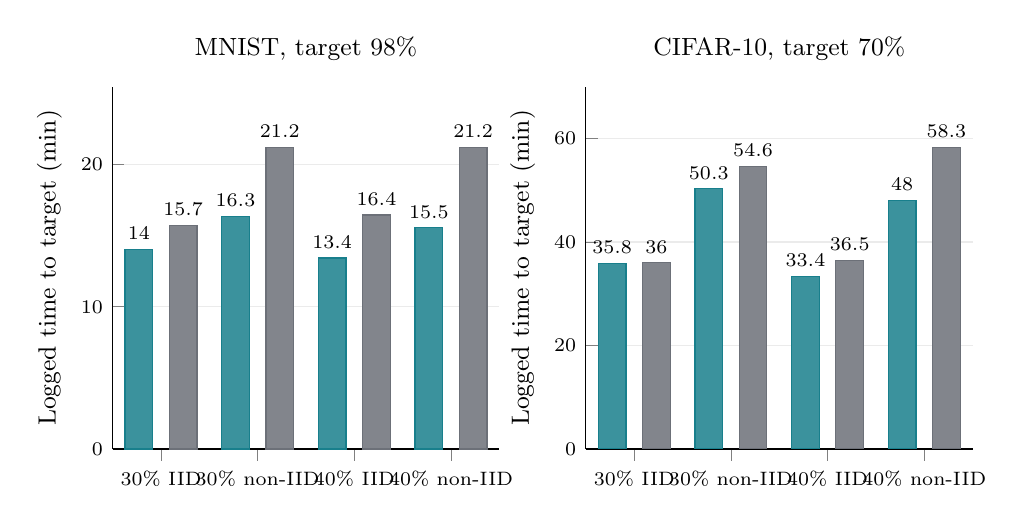
\begin{tikzpicture}
\begin{groupplot}[group style={group size=2 by 1,horizontal sep=1.1cm},scale only axis,width=0.405\textwidth,height=4.6cm,ybar,/pgf/bar width=10pt,xmin=0.5,xmax=4.5,ymin=0,xtick={1,2,3,4},xticklabels={{30\% IID},{30\% non-IID},{40\% IID},{40\% non-IID}},axis x line*=bottom,axis y line*=left,ymajorgrids=true,grid style={black!8},tick label style={font=\scriptsize},label style={font=\small},title style={font=\small},scaled y ticks=false,nodes near coords,every node near coord/.append style={font=\scriptsize,/pgf/number format/fixed,/pgf/number format/precision=1}]
\nextgroupplot[title={MNIST, target 98\%},ylabel={Logged time to target (min)},ymax=25.464683]
\addplot[/pgf/bar shift=-8pt,fill=baitteal!85,draw=baitteal] coordinates {(1,14.016757) (2,16.330195) (3,13.430266) (4,15.549999)};
\addplot[/pgf/bar shift=8pt,fill=comparisongray!85,draw=comparisongray] coordinates {(1,15.722327) (2,21.220569) (3,16.448178) (4,21.219035)};
\nextgroupplot[title={CIFAR-10, target 70\%},ylabel={Logged time to target (min)},ymax=69.978006]
\addplot[/pgf/bar shift=-8pt,fill=baitteal!85,draw=baitteal] coordinates {(1,35.797480) (2,50.272567) (3,33.358247) (4,48.018053)};
\addplot[/pgf/bar shift=8pt,fill=comparisongray!85,draw=comparisongray] coordinates {(1,35.964126) (2,54.618728) (3,36.459030) (4,58.315005)};
\end{groupplot}\end{tikzpicture}
\par\smallskip{\small\textcolor{baitteal}{\rule{0.35cm}{0.18cm}}\ BaitFL\qquad\textcolor{comparisongray}{\rule{0.35cm}{0.18cm}}\ No defense}
\caption{Time to first target-accuracy crossing in matched runs. BaitFL is the left bar and no defense the right bar in each pair.}\label{fig:time-target}
\end{figure*}

% END SOURCE: generated/time_target_figure.tex


\subsection{Instrumented Timing and Lightweight Operation}\label{sec:native-timing}
Dedicated executions compare BaitFL with a reimplementation of STD-DAGMM
on non-IID FR3 at 40\%, using both datasets, 100 clients,
100 rounds, three local epochs and six CPU threads. STD-DAGMM freshly
fits its auxiliary model for five epochs per round and retains every
client. That fitting budget is a declared reproduction choice, not an
author-specified training schedule or evidence of convergence
\cite{lin2019freeriders,zong2018dagmm}. The instrumented BaitFL run
matches its corresponding study accuracy trajectory in every round.

Table~\ref{tab:std-segments} separates training from response preparation,
challenge construction, decisions, aggregation and evaluation. BaitFL's
recorded challenge, feature/preparation and decision stages average
215.21 ms per round on MNIST and
791.03 ms on CIFAR-10. They account for 0.58\% and
0.89\% of the corresponding computation totals. STD-DAGMM adds auxiliary
fitting, averaging 15.76 and 42.09 seconds.
The checking subtotal groups these stages. The final rows give BaitFL's
absolute saving in seconds per round together with the percentage
reduction relative to STD-DAGMM. Stage times include sample standard
deviations across the 100 rounds, capturing variation between ordinary
training and periodic decisions.

Figure~\ref{fig:timing-phases} shows average
computation and elapsed round time over the complete horizon. BaitFL uses
29.35\% less computation time on MNIST and
26.23\% less on CIFAR-10 in these executions. Elapsed-time
reductions are 34.87\% and
27.20\%. Logging, checkpoints and other runtime costs
contribute to the difference between computation and elapsed time. Network
communication is absent from both measurements.

% BEGIN SOURCE: generated/timing_compact_table.tex
\begin{table*}[t]\centering\footnotesize\setlength{\tabcolsep}{4pt}
\caption{Round-time breakdown.}\label{tab:std-segments}
\begin{tabular}{lrrrr}\toprule
\multirow{2}{*}{Stage} & \multicolumn{2}{c}{MNIST} & \multicolumn{2}{c}{CIFAR-10} \\
\cmidrule(lr){2-3}\cmidrule(lr){4-5}
 & BaitFL & STD-DAGMM & BaitFL & STD-DAGMM \\ \midrule
Honest local training & $34.30 \pm 0.94$ & $33.89 \pm 0.66$ & $81.37 \pm 5.40$ & $72.42 \pm 3.68$ \\
Fabricated responses & $0.018 \pm 0.029$ & $0.066 \pm 0.011$ & $0.188 \pm 0.172$ & $0.224 \pm 0.022$ \\
Client diagnostic evaluation & $0.161 \pm 0.248$ & $0$ & $0.899 \pm 0.752$ & $0$ \\
Traps and scheduling & $0.0018 \pm 0.0055$ & $0$ & $0.018 \pm 0.058$ & $0$ \\
Response features and preparation & $0.198 \pm 0.050$ & $0.045 \pm 0.003$ & $0.729 \pm 0.179$ & $0.115 \pm 0.012$ \\
Auxiliary detector fitting & $0$ & $15.76 \pm 1.25$ & $0$ & $42.09 \pm 1.87$ \\
Scoring and state decisions & $0.016 \pm 0.071$ & $0.335 \pm 0.039$ & $0.043 \pm 0.145$ & $0.827 \pm 0.057$ \\
Aggregation & $0.030 \pm 0.013$ & $0.043 \pm 0.003$ & $0.096 \pm 0.039$ & $0.136 \pm 0.014$ \\
Global evaluation & $2.20 \pm 0.10$ & $2.13 \pm 0.04$ & $5.21 \pm 0.44$ & $4.24 \pm 0.20$ \\
\midrule
Logging and checkpoints & $3.99 \pm 0.61$ & $3.75 \pm 0.54$ & $11.34 \pm 1.79$ & $9.76 \pm 1.30$ \\
Unassigned runtime & $0.0088 \pm 0.0026$ & $6.82 \pm 2.33$ & $0.054 \pm 0.044$ & $7.49 \pm 2.08$ \\
\midrule
Checking subtotal (included above) & $0.215 \pm 0.093$ & $16.14 \pm 1.25$ & $0.791 \pm 0.244$ & $43.03 \pm 1.91$ \\
Checking share of computation (\%) & 0.58 & 30.89 & 0.89 & 35.84 \\
\midrule
\multicolumn{5}{l}{\textit{BaitFL time saved relative to STD-DAGMM}} \\
Computation saved: s/round (\%) & \multicolumn{2}{c}{15.34 (29.35\%)} & \multicolumn{2}{c}{31.50 (26.23\%)} \\
Elapsed saved: s/round (\%) & \multicolumn{2}{c}{21.91 (34.87\%)} & \multicolumn{2}{c}{37.35 (27.20\%)} \\
\bottomrule\end{tabular}
\par\smallskip\parbox{0.94\textwidth}{\scriptsize Times are mean $\pm$ sample SD in seconds per round over 100 rounds. Combined stages are summed per round before calculating SD. Checking subtotals are included in the preceding stages. Shares and savings use complete-horizon means, relative to STD-DAGMM for savings.}
\end{table*}

% END SOURCE: generated/timing_compact_table.tex


% BEGIN SOURCE: generated/timing_phases_figure.tex
\begin{figure*}[t]\centering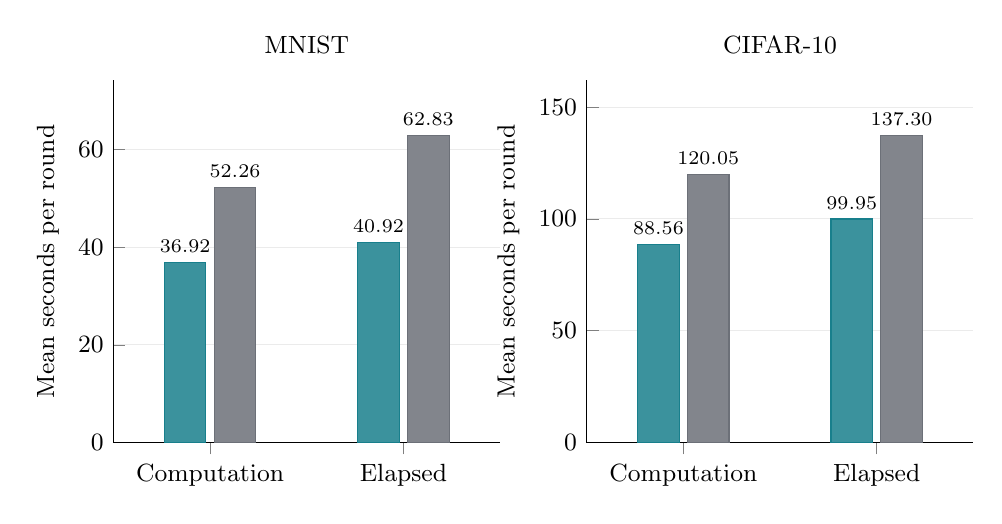
\begin{tikzpicture}
\begin{groupplot}[group style={group size=2 by 1,horizontal sep=1.1cm},scale only axis,width=0.405\textwidth,height=4.6cm,ybar,/pgf/bar width=15pt,xmin=0.5,xmax=2.5,ymin=0,xtick={1,2},xticklabels={{Computation},{Elapsed}},axis x line*=bottom,axis y line*=left,ymajorgrids=true,grid style={black!8},tick label style={font=\small},label style={font=\small},title style={font=\small},scaled y ticks=false,nodes near coords,every node near coord/.append style={font=\scriptsize,/pgf/number format/fixed,/pgf/number format/precision=2,/pgf/number format/fixed zerofill}]
\nextgroupplot[title={MNIST},ylabel={Mean seconds per round},ymax=74.1433]
\addplot[/pgf/bar shift=-9pt,fill=baitteal!85,draw=baitteal] coordinates {(1,36.920542) (2,40.923968)};
\addplot[/pgf/bar shift=9pt,fill=comparisongray!85,draw=comparisongray] coordinates {(1,52.261755) (2,62.833304)};
\nextgroupplot[title={CIFAR-10},ylabel={Mean seconds per round},ymax=162.0135]
\addplot[/pgf/bar shift=-9pt,fill=baitteal!85,draw=baitteal] coordinates {(1,88.558552) (2,99.952120)};
\addplot[/pgf/bar shift=9pt,fill=comparisongray!85,draw=comparisongray] coordinates {(1,120.053736) (2,137.299553)};
\end{groupplot}\end{tikzpicture}
\par\smallskip{\small\textcolor{baitteal}{\rule{0.35cm}{0.18cm}}\ BaitFL\qquad\textcolor{comparisongray}{\rule{0.35cm}{0.18cm}}\ STD-DAGMM}
\caption{Average computation and elapsed time per round.}\label{fig:timing-phases}
\end{figure*}

% END SOURCE: generated/timing_phases_figure.tex


These timing cases describe different native workflows. BaitFL changes
probing and participation, whereas STD-DAGMM keeps the full population.
Removing free riders does not remove honest clients' local SGD jobs.
Checking accounts for less than 1\% of measured computation,
while the STD-DAGMM comparison measures a particular fitting budget.
Detailed per-round and fitting-stage records accompany the study.

The stored STD-DAGMM flags also permit a limited diagnostic of this
five-epoch recipe. Each timing execution contains 4,000 free-rider
responses, none of which is flagged. The numbers of flagged honest
responses are 2,200 on MNIST and 2,196 on CIFAR-10, giving zero pooled
flag precision and recall in both executions. These are roundwise flags
from one configuration and fitting budget. A comparative detection
benchmark would require matched decision endpoints and baseline settings,
so these observations do not establish a ranking against BaitFL's
permanent-removal results.

The unassigned-runtime entry is the difference between elapsed time and
the sum of explicitly timed computation and I/O stages. Its larger value
for STD-DAGMM shows that the two execution paths include different
untimed work. It is excluded from computation totals and cannot be
attributed to detector fitting. Elapsed-time savings include this
difference, so they are not an isolated measure of detection overhead.

Low checking cost does not imply immediate detection.
Figure~\ref{fig:completion-rounds} shows the variation in complete-removal
rounds across configurations. Markers indicate the mean completion round,
with whiskers spanning the observed minimum and maximum.
The wider ranges in history-based attacks
reflect the additional challenge cycles sometimes needed for confirmation.

% BEGIN SOURCE: generated/completion_rounds_figure.tex
\begin{figure*}[tp]\centering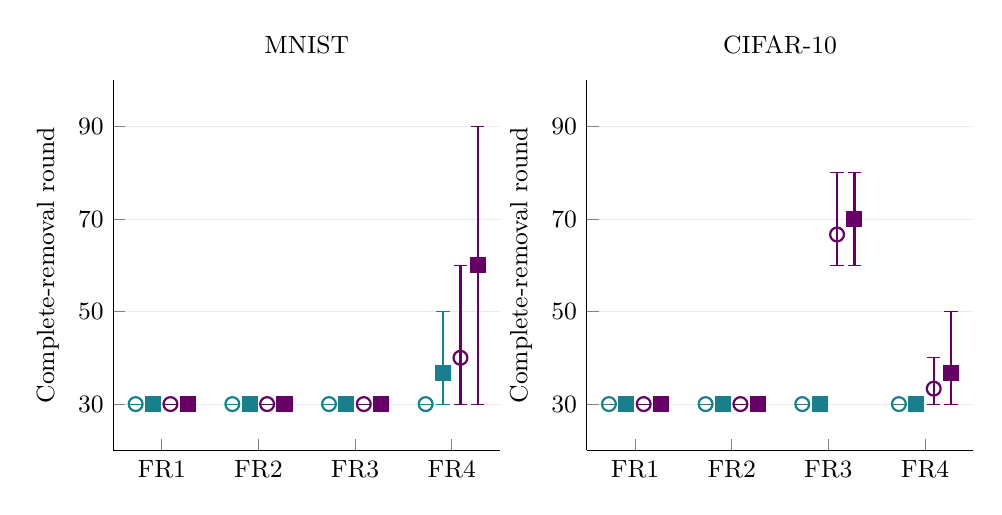
\begin{tikzpicture}
\begin{groupplot}[group style={group size=2 by 1,horizontal sep=1.1cm},scale only axis,width=0.405\textwidth,height=4.7cm,xmin=0.5,xmax=4.5,ymin=20,ymax=100,xtick={1,2,3,4},xticklabels={FR1,FR2,FR3,FR4},ytick={30,50,70,90},axis x line*=bottom,axis y line*=left,ymajorgrids=true,grid style={black!8},tick label style={font=\small},label style={font=\small},title style={font=\small},scaled y ticks=false]
\nextgroupplot[title={MNIST},ylabel={Complete-removal round}]
\addplot[only marks,baitteal,mark=o,mark options={fill=white},mark size=2.5pt,thick,error bars/.cd,y dir=both,y explicit,error bar style={line width=0.8pt},error mark options={rotate=90,mark size=2.4pt}] coordinates {(0.730,30.00000) += (0,0.00000) -= (0,0.00000) (1.730,30.00000) += (0,0.00000) -= (0,0.00000) (2.730,30.00000) += (0,0.00000) -= (0,0.00000) (3.730,30.00000) += (0,0.00000) -= (0,0.00000)};
\addplot[only marks,baitteal,mark=square*,mark options={fill=baitteal},mark size=2.5pt,thick,error bars/.cd,y dir=both,y explicit,error bar style={line width=0.8pt},error mark options={rotate=90,mark size=2.4pt}] coordinates {(0.910,30.00000) += (0,0.00000) -= (0,0.00000) (1.910,30.00000) += (0,0.00000) -= (0,0.00000) (2.910,30.00000) += (0,0.00000) -= (0,0.00000) (3.910,36.66667) += (0,13.33333) -= (0,6.66667)};
\addplot[only marks,violet!80!black,mark=o,mark options={fill=white},mark size=2.5pt,thick,error bars/.cd,y dir=both,y explicit,error bar style={line width=0.8pt},error mark options={rotate=90,mark size=2.4pt}] coordinates {(1.090,30.00000) += (0,0.00000) -= (0,0.00000) (2.090,30.00000) += (0,0.00000) -= (0,0.00000) (3.090,30.00000) += (0,0.00000) -= (0,0.00000) (4.090,40.00000) += (0,20.00000) -= (0,10.00000)};
\addplot[only marks,violet!80!black,mark=square*,mark options={fill=violet!80!black},mark size=2.5pt,thick,error bars/.cd,y dir=both,y explicit,error bar style={line width=0.8pt},error mark options={rotate=90,mark size=2.4pt}] coordinates {(1.270,30.00000) += (0,0.00000) -= (0,0.00000) (2.270,30.00000) += (0,0.00000) -= (0,0.00000) (3.270,30.00000) += (0,0.00000) -= (0,0.00000) (4.270,60.00000) += (0,30.00000) -= (0,30.00000)};
\nextgroupplot[title={CIFAR-10},ylabel={Complete-removal round}]
\addplot[only marks,baitteal,mark=o,mark options={fill=white},mark size=2.5pt,thick,error bars/.cd,y dir=both,y explicit,error bar style={line width=0.8pt},error mark options={rotate=90,mark size=2.4pt}] coordinates {(0.730,30.00000) += (0,0.00000) -= (0,0.00000) (1.730,30.00000) += (0,0.00000) -= (0,0.00000) (2.730,30.00000) += (0,0.00000) -= (0,0.00000) (3.730,30.00000) += (0,0.00000) -= (0,0.00000)};
\addplot[only marks,baitteal,mark=square*,mark options={fill=baitteal},mark size=2.5pt,thick,error bars/.cd,y dir=both,y explicit,error bar style={line width=0.8pt},error mark options={rotate=90,mark size=2.4pt}] coordinates {(0.910,30.00000) += (0,0.00000) -= (0,0.00000) (1.910,30.00000) += (0,0.00000) -= (0,0.00000) (2.910,30.00000) += (0,0.00000) -= (0,0.00000) (3.910,30.00000) += (0,0.00000) -= (0,0.00000)};
\addplot[only marks,violet!80!black,mark=o,mark options={fill=white},mark size=2.5pt,thick,error bars/.cd,y dir=both,y explicit,error bar style={line width=0.8pt},error mark options={rotate=90,mark size=2.4pt}] coordinates {(1.090,30.00000) += (0,0.00000) -= (0,0.00000) (2.090,30.00000) += (0,0.00000) -= (0,0.00000) (3.090,66.66667) += (0,13.33333) -= (0,6.66667) (4.090,33.33333) += (0,6.66667) -= (0,3.33333)};
\addplot[only marks,violet!80!black,mark=square*,mark options={fill=violet!80!black},mark size=2.5pt,thick,error bars/.cd,y dir=both,y explicit,error bar style={line width=0.8pt},error mark options={rotate=90,mark size=2.4pt}] coordinates {(1.270,30.00000) += (0,0.00000) -= (0,0.00000) (2.270,30.00000) += (0,0.00000) -= (0,0.00000) (3.270,70.00000) += (0,10.00000) -= (0,10.00000) (4.270,36.66667) += (0,13.33333) -= (0,6.66667)};
\end{groupplot}\end{tikzpicture}
\par\smallskip{\small\textcolor{baitteal}{$\circ$}\ 30\% IID\quad\textcolor{baitteal}{$\blacksquare$}\ 40\% IID\quad\textcolor{violet!80!black}{$\circ$}\ 30\% non-IID\quad\textcolor{violet!80!black}{$\blacksquare$}\ 40\% non-IID}
\caption{Free-rider removal completion rounds.}\label{fig:completion-rounds}
\end{figure*}

% END SOURCE: generated/completion_rounds_figure.tex


\section{Complexity and Lightweight Design}\label{sec:complexity}
Let $N$ be the largest active population, $P$ the floating model coordinates,
$L$ the floating tensors, $B$ bootstrap replicates and
$K=\lceil\sqrt N\rceil$ bins. Feature extraction reads $O(NP)$ coordinates
per round. Leave-one-out profile comparisons cost $O(N^2L)$, with
$O(N^2\log N)$ additional scalar-median work in the current implementation.
Bootstrap splitting costs $O(B(N+K))$ on scalars. For $T$ rounds, $M$
paired cycles and $A$ sparse audits, total incremental detector work is
\begin{equation}\label{eq:detector-work}
\begin{aligned}
\mathcal W_{\rm det}=O\bigl(&TNP+(M+A)\bigl[N^2(L+\log N)\\
&\hspace{4em}+B(N+K)\bigr]\bigr).
\end{aligned}
\end{equation}
Equation~\eqref{eq:detector-work} excludes ordinary training, aggregation
and persistent logging. The detector is linear in model size for feature
extraction and quadratic in client count for peer comparisons; it is not
claimed to scale linearly in the federation population.

Working state is $O(P+NL+BN+BK)$, plus $O(N)$ evidence counters and
fingerprints. At 100 clients, packed paired summaries occupy about
8.59 KiB on MNIST and 19.53 KiB on CIFAR-10. Shared float32 challenges
occupy about 1.58 and 4.74 MiB. Python objects, temporary arrays, client
models and attacker histories make full-process RSS larger. Supplementary
Tables S3--S4 give operation-level bounds and payload calculations.

Challenges replace ordinary model requests, so the nominal payload order
remains $O(NP)$ per round. Withholding genuine responses can change time
to target accuracy. No network or energy saving follows from unchanged
payload order. The measured sub-1\% checking fractions support lightweight
server computation only for the tested population and architectures.

\section{Discussion and Limitations}\label{sec:discussion}
\subsection{Information Available to the Server}
BaitFL uses returned models, client and challenge identifiers, response
norms, profile distances and exact-sendback checks. Attacker identities
and behavior settings belong to the simulator and evaluation records.
They do not enter screening, geometric tests or confirmation. Likewise,
the configured attacker proportion does not set a removal quota.
This separation prevents direct use of evaluation labels, although the
method's design has been informed by experimental observations.

\subsection{Confirmation and Honest-Client Safety}
Statistical removal requires fresh evidence from the same component
on both selected challenges and in another complete cycle. Mixed
norm/profile findings cannot be combined to reach confirmation, and
stored evidence alone cannot authorize removal. Paired exact sendback
also requires repetition. Weak unresolved labels do not renew quarantine,
and unconfirmed review expires when fresh strong evidence does not recur.

These rules reduce reliance on isolated anomalies. They do not make
repeated evidence statistically independent. An honest client keeps
its local data across challenges and can therefore remain unusual in
successive cycles. Certificate memory can accumulate such findings
unless two complete clear cycles reset it, explaining the risk of late
false removal observed in the experiments.

The decision boundaries are derived from the observed population rather
than an attack-fitted numerical z-score cutoff. Nevertheless, the method
has design parameters, including challenge strength, bootstrap confidence,
cohort support and confirmation lengths. At 100 clients, statistical
certification requires a cohort of at least ten. A small group of free
riders that avoids exact sendback may therefore remain uncertified.

\subsection{Adaptive Attacks and Identifiability}\label{sec:evasion}
A response-only detector cannot distinguish two clients whose observable
histories are identical, even if one trained and the other fabricated
its responses. BaitFL therefore tests whether challenges expose
differences in behavior. Its certificates do not prove that local
computation occurred.

The evaluated free riders are not told which models are challenges.
An adaptive participant might still recognize repeated frozen models,
unusual perturbations or differences revealed through communication with
other clients. Reproducible simulation randomness also does not establish
unpredictability against an attacker who knows its configuration.
Deployment would require server-secret randomness and tests against
challenge-aware strategies. Secrecy alone would not guarantee that
challenge models are indistinguishable from ordinary ones.

\subsection{Privacy and Participation Limits}
The server inspects individual returned models, so the current protocol
cannot be used directly with standard secure
aggregation~\cite{bonawitz2017practical}. It does not access raw client
data or require reported training loss, but these restrictions do not
provide differential privacy or prevent information leakage through
updates~\cite{kairouz2021advances,zhu2019leakage,melis2019leakage}.

The reference population assumes an honest majority. Colluding clients
could share trained responses, while Sybil identities could distort the
reference distribution. Neither case is evaluated. The experiments also
assume complete participation. Incomplete challenge coverage cannot
certify removal, and the simulator stops on a nonfinite response rather
than providing a full malicious-message or dropout-handling protocol.
Checkpoint recovery restores the recorded training and evidence state
after an interruption. Authentication and availability defenses require
additional mechanisms.

\subsection{Evaluation Scope and Remaining Tests}
The main grid covers three seeds, 100 clients, one architecture per dataset
and one non-IID concentration. The new lower-prevalence checks use one
frozen seed and expose misses at 5\%; they do not support a prevalence-
independent recall claim. The norm-matching feature diagnostic isolates
statistical behavior but is not a full adaptive attack. Component and
passive-detector ablations, completed published-attack runs and a stronger
detection baseline are still needed. The stored five-epoch STD-DAGMM
recipe supplies flag diagnostics, not a fair ranking of detection methods.

Future tests should vary local training, non-IID concentration, model
architecture, BatchNorm-buffer treatment, collusion and participation.
LEAF and FedScale provide relevant heterogeneous settings
\cite{caldas2018leaf,lai2022fedscale}. The held-out seed phase is registered
but unexecuted. Oracle utility comparisons are also pending, so the
benefit of removing fabricated responses is not yet separated from the
cost of withholding honest challenge responses. Larger-scale detector
memory, communication and energy measurements remain necessary.

\subsection{Code and Evidence Availability}
The project repository is available at\par
{\footnotesize\urlstyle{same}\url{https://github.com/Aashnan-Rahman/Mitigating-Free-Rider}}\par
The study retains configurations, per-client decisions, per-round timing
and source hashes for reproducibility. A public immutable archive of
the exact manuscript evidence is not yet available.

\section{Conclusion}
BaitFL combines model challenges, compact response statistics and repeated
fresh evidence. The 96-run 30\%/40\% grid removes all tested free riders,
with three honest removals in two runs. Four additional honest-only runs
have no honest removal, but the completed non-IID 5\% tests miss FR2--FR4.
These outcomes delimit the support gate's operating range rather than
establish universal recall. The norm-matching diagnostic further tests
what magnitude contrast alone cannot establish. Checking remains below
1\% of computation in the two instrumented workflows. Reliable auditing
under lower prevalence, stronger fabrication and heterogeneous honest
behavior remains the central research problem.



% BEGIN SOURCE: build/paper_v7_2.bbl
\begin{thebibliography}{10}
\providecommand{\url}[1]{#1}
\csname url@samestyle\endcsname
\providecommand{\newblock}{\relax}
\providecommand{\bibinfo}[2]{#2}
\providecommand{\BIBentrySTDinterwordspacing}{\spaceskip=0pt\relax}
\providecommand{\BIBentryALTinterwordstretchfactor}{4}
\providecommand{\BIBentryALTinterwordspacing}{\spaceskip=\fontdimen2\font plus
\BIBentryALTinterwordstretchfactor\fontdimen3\font minus
  \fontdimen4\font\relax}
\providecommand{\BIBforeignlanguage}[2]{{%
\expandafter\ifx\csname l@#1\endcsname\relax
\typeout{** WARNING: IEEEtran.bst: No hyphenation pattern has been}%
\typeout{** loaded for the language `#1'. Using the pattern for}%
\typeout{** the default language instead.}%
\else
\language=\csname l@#1\endcsname
\fi
#2}}
\providecommand{\BIBdecl}{\relax}
\BIBdecl

\bibitem{mcmahan2017communication}
\BIBentryALTinterwordspacing
H.~B. McMahan, E.~Moore, D.~Ramage, S.~Hampson, and B.~{Ag{\"u}era y Arcas},
  ``Communication-efficient learning of deep networks from decentralized
  data,'' in \emph{Proceedings of the 20th International Conference on
  Artificial Intelligence and Statistics}, ser. Proceedings of Machine Learning
  Research, vol.~54.\hskip 1em plus 0.5em minus 0.4em\relax PMLR, 2017, pp.
  1273--1282. [Online]. Available:
  \url{https://proceedings.mlr.press/v54/mcmahan17a.html}
\BIBentrySTDinterwordspacing

\bibitem{kairouz2021advances}
\BIBentryALTinterwordspacing
P.~Kairouz, H.~B. McMahan, B.~Avent \emph{et~al.}, ``Advances and open problems
  in federated learning,'' \emph{Foundations and Trends in Machine Learning},
  vol.~14, no. 1--2, pp. 1--210, 2021. [Online]. Available:
  \url{https://arxiv.org/abs/1912.04977}
\BIBentrySTDinterwordspacing

\bibitem{zhu2019leakage}
\BIBentryALTinterwordspacing
L.~Zhu, Z.~Liu, and S.~Han, ``Deep leakage from gradients,'' in \emph{Advances
  in Neural Information Processing Systems}, vol.~32, 2019. [Online].
  Available:
  \url{https://proceedings.neurips.cc/paper_files/paper/2019/hash/60a6c4002cc7b29142def8871531281a-Abstract.html}
\BIBentrySTDinterwordspacing

\bibitem{melis2019leakage}
\BIBentryALTinterwordspacing
L.~Melis, C.~Song, E.~D. Cristofaro, and V.~Shmatikov, ``Exploiting unintended
  feature leakage in collaborative learning,'' in \emph{IEEE Symposium on
  Security and Privacy}, 2019, pp. 691--706. [Online]. Available:
  \url{https://doi.org/10.1109/SP.2019.00029}
\BIBentrySTDinterwordspacing

\bibitem{bagdasaryan2020backdoor}
\BIBentryALTinterwordspacing
E.~Bagdasaryan, A.~Veit, Y.~Hua, D.~Estrin, and V.~Shmatikov, ``How to backdoor
  federated learning,'' in \emph{Proceedings of the Twenty Third International
  Conference on Artificial Intelligence and Statistics}, ser. Proceedings of
  Machine Learning Research, vol. 108.\hskip 1em plus 0.5em minus 0.4em\relax
  PMLR, 2020, pp. 2938--2948. [Online]. Available:
  \url{https://proceedings.mlr.press/v108/bagdasaryan20a.html}
\BIBentrySTDinterwordspacing

\bibitem{lin2019freeriders}
\BIBentryALTinterwordspacing
J.~Lin, M.~Du, and J.~Liu, ``Free-riders in federated learning: Attacks and
  defenses,'' arXiv preprint arXiv:1911.12560, 2019. [Online]. Available:
  \url{https://arxiv.org/abs/1911.12560}
\BIBentrySTDinterwordspacing

\bibitem{fraboni2021freerider}
\BIBentryALTinterwordspacing
Y.~Fraboni, R.~Vidal, and M.~Lorenzi, ``Free-rider attacks on model aggregation
  in federated learning,'' in \emph{Proceedings of the 24th International
  Conference on Artificial Intelligence and Statistics}, ser. Proceedings of
  Machine Learning Research, vol. 130.\hskip 1em plus 0.5em minus 0.4em\relax
  PMLR, 2021, pp. 1846--1854. [Online]. Available:
  \url{https://proceedings.mlr.press/v130/fraboni21a.html}
\BIBentrySTDinterwordspacing

\bibitem{wang2024pass}
\BIBentryALTinterwordspacing
J.~Wang, X.~Chang, J.~Mi{\v{s}}i{\'c}, V.~B. Mi{\v{s}}i{\'c}, and Y.~Wang,
  ``{PASS}: A parameter audit-based secure and fair federated learning scheme
  against free-rider attack,'' \emph{IEEE Internet of Things Journal}, vol.~11,
  no.~1, pp. 1374--1384, 2024. [Online]. Available:
  \url{https://doi.org/10.1109/JIOT.2023.3288936}
\BIBentrySTDinterwordspacing

\bibitem{recasens2026frida}
\BIBentryALTinterwordspacing
P.~G. Recasens, {\'A}.~Horv{\'a}th, A.~Gutierrez-Torre, J.~Torres, J.~L.
  Berral, and B.~Pej{\'o}, ``{FRIDA}: Free-rider detection using privacy
  attacks,'' \emph{Journal of Information Security and Applications}, vol.~97,
  2026, art. no. 104357. [Online]. Available:
  \url{https://doi.org/10.1016/j.jisa.2025.104357}
\BIBentrySTDinterwordspacing

\bibitem{zong2018dagmm}
\BIBentryALTinterwordspacing
B.~Zong, Q.~Song, M.~R. Min, W.~Cheng, C.~Lumezanu, D.~Cho, and H.~Chen, ``Deep
  autoencoding gaussian mixture model for unsupervised anomaly detection,'' in
  \emph{International Conference on Learning Representations}, 2018. [Online].
  Available: \url{https://openreview.net/forum?id=BJJLHbb0-}
\BIBentrySTDinterwordspacing

\bibitem{zhu2021advanced}
\BIBentryALTinterwordspacing
Z.~Zhu, J.~Shu, X.~Zou, and X.~Jia, ``Advanced free-rider attacks in federated
  learning,'' in \emph{NeurIPS Workshop on New Frontiers in Federated
  Learning}, 2021. [Online]. Available:
  \url{https://neurips2021workshopfl.github.io/NFFL-2021/papers/2021/Zhu2021.pdf}
\BIBentrySTDinterwordspacing

\bibitem{wang2024frad}
\BIBentryALTinterwordspacing
B.~Wang, H.~Li, X.~Liu, and Y.~Guo, ``{FRAD}: Free-rider attacks detection
  mechanism for federated learning in {AIoT},'' \emph{IEEE Internet of Things
  Journal}, vol.~11, no.~3, pp. 4377--4388, 2024. [Online]. Available:
  \url{https://doi.org/10.1109/JIOT.2023.3298606}
\BIBentrySTDinterwordspacing

\bibitem{bonawitz2017practical}
\BIBentryALTinterwordspacing
K.~Bonawitz, V.~Ivanov, B.~Kreuter, A.~Marcedone, H.~B. McMahan, S.~Patel,
  D.~Ramage, A.~Segal, and K.~Seth, ``Practical secure aggregation for
  privacy-preserving machine learning,'' in \emph{Proceedings of the 2017 ACM
  SIGSAC Conference on Computer and Communications Security}, 2017, pp.
  1175--1191. [Online]. Available:
  \url{https://research.google/pubs/practical-secure-aggregation-for-privacy-preserving-machine-learning/}
\BIBentrySTDinterwordspacing

\bibitem{blanchard2017krum}
\BIBentryALTinterwordspacing
P.~Blanchard, E.~M.~E. Mhamdi, R.~Guerraoui, and J.~Stainer, ``Machine learning
  with adversaries: Byzantine tolerant gradient descent,'' in \emph{Advances in
  Neural Information Processing Systems}, vol.~30, 2017. [Online]. Available:
  \url{https://proceedings.neurips.cc/paper/6617-machine-learning-with-adversaries-byzantine-tolerant-gradient-descent.pdf}
\BIBentrySTDinterwordspacing

\bibitem{yin2018byzantine}
\BIBentryALTinterwordspacing
D.~Yin, Y.~Chen, K.~Ramchandran, and P.~Bartlett, ``Byzantine-robust
  distributed learning: Towards optimal statistical rates,'' in
  \emph{Proceedings of the 35th International Conference on Machine Learning},
  ser. Proceedings of Machine Learning Research, vol.~80, 2018, pp. 5650--5659.
  [Online]. Available: \url{https://proceedings.mlr.press/v80/yin18a.html}
\BIBentrySTDinterwordspacing

\bibitem{pillutla2022rfa}
\BIBentryALTinterwordspacing
K.~Pillutla, S.~M. Kakade, and Z.~Harchaoui, ``Robust aggregation for federated
  learning,'' \emph{IEEE Transactions on Signal Processing}, vol.~70, pp.
  1142--1154, 2022. [Online]. Available:
  \url{https://doi.org/10.1109/TSP.2022.3153135}
\BIBentrySTDinterwordspacing

\bibitem{cao2021fltrust}
\BIBentryALTinterwordspacing
X.~Cao, M.~Fang, J.~Liu, and N.~Z. Gong, ``{FLTrust}: Byzantine-robust
  federated learning via trust bootstrapping,'' in \emph{Network and
  Distributed System Security Symposium}, 2021. [Online]. Available:
  \url{https://www.ndss-symposium.org/wp-content/uploads/ndss2021_6C-2_24434_paper.pdf}
\BIBentrySTDinterwordspacing

\bibitem{li2020fedprox}
\BIBentryALTinterwordspacing
T.~Li, A.~K. Sahu, M.~Zaheer, M.~Sanjabi, A.~Talwalkar, and V.~Smith,
  ``Federated optimization in heterogeneous networks,'' in \emph{Proceedings of
  Machine Learning and Systems}, vol.~2, 2020. [Online]. Available:
  \url{https://proceedings.mlsys.org/paper_files/paper/2020/hash/1f5fe83998a09396ebe6477d9475ba0c-Abstract.html}
\BIBentrySTDinterwordspacing

\bibitem{karimireddy2020scaffold}
\BIBentryALTinterwordspacing
S.~P. Karimireddy, S.~Kale, M.~Mohri, S.~Reddi, S.~Stich, and A.~T. Suresh,
  ``{SCAFFOLD}: Stochastic controlled averaging for federated learning,'' in
  \emph{Proceedings of the 37th International Conference on Machine Learning},
  ser. Proceedings of Machine Learning Research, vol. 119, 2020, pp.
  5132--5143. [Online]. Available:
  \url{https://proceedings.mlr.press/v119/karimireddy20a.html}
\BIBentrySTDinterwordspacing

\bibitem{wang2020fednova}
\BIBentryALTinterwordspacing
J.~Wang, Q.~Liu, H.~Liang, G.~Joshi, and H.~V. Poor, ``Tackling the objective
  inconsistency problem in heterogeneous federated optimization,'' in
  \emph{Advances in Neural Information Processing Systems}, vol.~33, 2020.
  [Online]. Available:
  \url{https://papers.neurips.cc/paper_files/paper/2020/hash/564127c03caab942e503ee6f810f54fd-Abstract.html}
\BIBentrySTDinterwordspacing

\bibitem{jia2021prooflearning}
\BIBentryALTinterwordspacing
H.~Jia, M.~Yaghini, C.~A. Choquette-Choo, N.~Dullerud, A.~Thudi,
  V.~Chandrasekaran, and N.~Papernot, ``Proof-of-learning: Definitions and
  practice,'' in \emph{IEEE Symposium on Security and Privacy}, 2021, pp.
  1039--1056. [Online]. Available: \url{https://arxiv.org/abs/2103.05633}
\BIBentrySTDinterwordspacing

\bibitem{zhao2021veriml}
\BIBentryALTinterwordspacing
L.~Zhao, Q.~Wang, C.~Wang, Q.~Li, C.~Shen, and B.~Feng, ``{VeriML}: Enabling
  integrity assurances and fair payments for machine learning as a service,''
  \emph{IEEE Transactions on Parallel and Distributed Systems}, vol.~32,
  no.~10, pp. 2524--2540, Oct. 2021. [Online]. Available:
  \url{https://doi.org/10.1109/TPDS.2021.3068195}
\BIBentrySTDinterwordspacing

\bibitem{ghorbani2019datashapley}
\BIBentryALTinterwordspacing
A.~Ghorbani and J.~Zou, ``Data shapley: Equitable valuation of data for machine
  learning,'' in \emph{Proceedings of the 36th International Conference on
  Machine Learning}, ser. Proceedings of Machine Learning Research, vol.~97,
  2019, pp. 2242--2251. [Online]. Available:
  \url{https://proceedings.mlr.press/v97/ghorbani19c.html}
\BIBentrySTDinterwordspacing

\bibitem{jia2019datavaluation}
\BIBentryALTinterwordspacing
R.~Jia, D.~Dao, B.~Wang, F.~A. Hubis, N.~Hynes, N.~M. Gurel, B.~Li, C.~Zhang,
  D.~Song, and C.~Spanos, ``Towards efficient data valuation based on the
  shapley value,'' in \emph{Proceedings of the 22nd International Conference on
  Artificial Intelligence and Statistics}, ser. Proceedings of Machine Learning
  Research, vol.~89, 2019, pp. 1167--1176. [Online]. Available:
  \url{https://proceedings.mlr.press/v89/jia19a.html}
\BIBentrySTDinterwordspacing

\bibitem{liu2022gtgshapley}
\BIBentryALTinterwordspacing
Z.~Liu, Y.~Chen, H.~Yu, Y.~Liu, and L.~Cui, ``{GTG-Shapley}: Efficient and
  accurate participant contribution evaluation in federated learning,''
  \emph{ACM Transactions on Intelligent Systems and Technology}, vol.~13,
  no.~4, 2022, art. no. 60. [Online]. Available:
  \url{https://arxiv.org/abs/2109.02053}
\BIBentrySTDinterwordspacing

\bibitem{otsu1979threshold}
\BIBentryALTinterwordspacing
N.~Otsu, ``A threshold selection method from gray-level histograms,''
  \emph{IEEE Transactions on Systems, Man, and Cybernetics}, vol.~9, no.~1, pp.
  62--66, 1979. [Online]. Available:
  \url{https://doi.org/10.1109/TSMC.1979.4310076}
\BIBentrySTDinterwordspacing

\bibitem{efron1979bootstrap}
\BIBentryALTinterwordspacing
B.~Efron, ``Bootstrap methods: Another look at the jackknife,'' \emph{The
  Annals of Statistics}, vol.~7, no.~1, pp. 1--26, 1979. [Online]. Available:
  \url{https://doi.org/10.1214/aos/1176344552}
\BIBentrySTDinterwordspacing

\bibitem{lecun1998gradient}
\BIBentryALTinterwordspacing
Y.~LeCun, L.~Bottou, Y.~Bengio, and P.~Haffner, ``Gradient-based learning
  applied to document recognition,'' \emph{Proceedings of the IEEE}, vol.~86,
  no.~11, pp. 2278--2324, 1998. [Online]. Available:
  \url{https://doi.org/10.1109/5.726791}
\BIBentrySTDinterwordspacing

\bibitem{krizhevsky2009learning}
\BIBentryALTinterwordspacing
A.~Krizhevsky, ``Learning multiple layers of features from tiny images,''
  University of Toronto, Tech. Rep., 2009. [Online]. Available:
  \url{https://www.cs.toronto.edu/~kriz/cifar.html}
\BIBentrySTDinterwordspacing

\bibitem{caldas2018leaf}
\BIBentryALTinterwordspacing
S.~Caldas, S.~M.~K. Duddu, P.~Wu, T.~Li, J.~Kone{\v{c}}n{\'y}, H.~B. McMahan,
  V.~Smith, and A.~Talwalkar, ``{LEAF}: A benchmark for federated settings,''
  arXiv preprint arXiv:1812.01097, 2018. [Online]. Available:
  \url{https://arxiv.org/abs/1812.01097}
\BIBentrySTDinterwordspacing

\bibitem{lai2022fedscale}
\BIBentryALTinterwordspacing
F.~Lai, Y.~Dai, S.~Singapuram, J.~Liu, X.~Zhu, H.~Madhyastha, and M.~Chowdhury,
  ``{FedScale}: Benchmarking model and system performance of federated learning
  at scale,'' in \emph{Proceedings of the 39th International Conference on
  Machine Learning}, ser. Proceedings of Machine Learning Research, vol. 162,
  2022, pp. 11\,814--11\,827. [Online]. Available:
  \url{https://proceedings.mlr.press/v162/lai22a.html}
\BIBentrySTDinterwordspacing

\end{thebibliography}

% END SOURCE: build/paper_v7_2.bbl

\end{document}
